\documentclass[nonatbib]{macrothesis}
\usepackage{amsmath,amssymb,amsfonts}
\usepackage{siunitx}
\usepackage{import}
\usepackage{enumitem}
\usepackage[authoryear,round]{natbib}
\usepackage{thmtools}
\usepackage[capitalize,nameinlink]{cleveref}
\usepackage{adjustbox}
\usepackage{subcaption}
\usepackage[toc,titletoc]{appendix}
\usepackage{algorithm}
\usepackage{algpseudocode}
\numberwithin{algorithm}{chapter}

\title{Title of the Thesis}
\author{Felipe Bartelt de Assis Pessoa}
\advisorname{Luciano Cunha de Araújo Pimenta}
\coadvisorname{Vinicius Mariano Gonçalves}
\departmentname{Department of Electrical Engineering}
\universityname{Universidade Federal de Minas Gerais}
\researchgroupname{MACRO Research Group - Mechatronics, Control, and Robotics}
\programname{Graduate Program in Electrical Engineering}
\locationname{Belo Horizonte, Brazil}

%%% Preambles %%%
% Dedication and Acknowledgments
\dedication{To my family.}
\acknowledgments{
    This is an acknowledgments. If you are using another language as main 
    (not english), then you should use this command as following:

    ``\textbackslash acknowledgments[Acknowledgments in your language]\{Text\}''
}

% Abstracts (in both languages)
\abstract{
    This is the abstract in the first language. If you are using another language as main
    (not english), then you should use this command as following:

    ``\textbackslash abstract[Abstract in your language]\{Text\}''

    \noindent(We used a typo to illustrate this feature here.)
}
\abstractsecond{
    Esse é um exemplo de abstract. Caso sua segunda língua não seja português,
    você deve usar o comando da seguinte forma:

    ``\textbackslash abstractsecond[Abstract in second language]\{Text\}''
}

\newlist{property}{enumerate}{1}
\newlist{feature}{enumerate}{1}
\setlist[property]{label=\roman{propertyi}, ref=\thedefinition.\roman{propertyi},noitemsep}
\setlist[feature]{label=(\alph*), ref=(\alph*),noitemsep}

\declaretheoremstyle[
  % spaceabove=\topsep, spacebelow=\topsep,
  % headfont=\normalfont\scshape,
  % notefont=\mdseries, notebraces={(}{)},
  % bodyfont=\normalfont,
  % postheadspace=1em,
  qed=\qedsymbol
]{defnstyle}

\declaretheorem[name=Theorem,numberwithin=chapter]{theorem}
\declaretheorem[name=Proposition,numberwithin=chapter,sibling=theorem]{proposition}
\declaretheorem[name=Lemma,numberwithin=chapter,sibling=theorem]{lemma}
\declaretheorem[name=Corollary,numberwithin=chapter,sibling=theorem]{corollary}
\declaretheorem[name=Example,numberwithin=chapter,sibling=theorem,style=defnstyle]{example}
\declaretheorem[name=Remark,numberwithin=chapter,sibling=theorem,style=defnstyle]{remark}
\declaretheorem[name=Definition,numberwithin=chapter,sibling=theorem,style=defnstyle]{definition}

\Crefname{theorem}{Theorem}{Theorems}
\Crefname{proposition}{Proposition}{Propositions}
\Crefname{lemma}{Lemma}{Lemmas}
\Crefname{definition}{Definition}{Definitions}
\Crefname{corollary}{Corollary}{Corollaries}
\Crefname{listprop}{Property}{Properties}
\Crefname{example}{Example}{Examples}
\Crefname{remark}{Remark}{Remarks}
\addtotheorempostheadhook[definition]{\crefalias{propertyi}{listprop}}
\crefname{featurei}{Feature}{Features}

\DeclareMathOperator{\Log}{Log}
\DeclareMathOperator{\tr}{tr}
\DeclareMathOperator{\vecop}{vec}


\DeclareRobustCommand{\SL}[1][]{%
  \!\;\mathcal{S}%
  \if\relax\detokenize{#1}\relax%
  \else%
    \!\left(#1\right)%
  \fi%
}
\DeclareRobustCommand{\invSL}[1][]{%
  \!\;\mathcal{S}^{-1}%
  \if\relax\detokenize{#1}\relax%
  \else%
    \!\left(#1\right)%
  \fi%
}

% !TeX root = main.tex

%----------------------------------------------------------------------------------------
%	Acronyms
%----------------------------------------------------------------------------------------
\newacronym{dof}{DoF}{Degree of Freedom}
\newacronym{uav}{UAV}{Unmanned Aerial Vehicle}
\newacronym{rgb}{RGB}{Red, Green, and Blue}
\newacronym{eedistacro}{EE}{Element-Element}
\newacronym{ecdistacro}{EC}{Element-Curve}
\newacronym{mrac}{MRAC}{Model Reference Adaptive Control}
%----------------------------------------------------------------------------------------
%	Notation
%----------------------------------------------------------------------------------------
%% Notation for Lie theory
\newnotation{G}{$G$}{Lie group}
\newnotation{GL}{$\text{GL}(n, \mathbb{R})$, $\text{GL}(n, \mathbb{C})$}{General Linear group of dimension $n$ over the real numbers, General Linear group of dimension $n$ over the complex numbers}
\newnotation{SL}{$\text{SL}(n, \mathbb{R})$, $\text{SL}(n, \mathbb{C})$}{Special Linear group of dimension $n$ over the real numbers, Special Linear group of dimension $n$ over the complex numbers}
\newnotation{SO}{$\text{O}(n)$, $\text{SO}(n)$}{Orthogonal group of dimension $n$, Special Orthogonal group of dimension $n$}
\newnotation{SE}{$\text{E}(n)$, $\text{SE}(n)$}{Euclidean group of dimension $n$, Special Euclidean group of dimension $n$}
\newnotation{Translgroup}{$\text{T}(n)$}{Translation group of dimension $n$. Matrix representation of $(\mathbb{R}^n, +)$}
\newnotation{isegroup}{$\text{ISE}(n)$}{Independent Special Euclidean group of dimension $n$, isomorphic to $\mathbb{R}^n\times\text{SO}(n)$}
\newnotation{sympgroup}{$\text{Sp}(2n)$}{Real Symplectic group of dimension $2n$}
\newnotation{indefort}{$\text{O}(p,q)$, $\text{SO}(p,q)$}{Indefinite Orthogonal group of signature $(p,q)$, Indefinite Special Orthogonal group of signature $(p,q)$}
\newnotation{lorentz}{$\text{O}(1, 3)$, $\text{SO}(1, 3)$, $\text{SO}^+(1, 3)$}{full Lorentz group, special Lorentz group, proper orthochronous Lorentz group}
\newnotation{g}{$\mathfrak{g}$}{Lie algebra of a Lie group $G$}
\newnotation{lieG}{$\text{Lie}(G)$}{Space of left-invariant, or right-invariant, vector fields on a Lie group $G$. Isomorphic to $\mathfrak{g}$}
\newnotation{gl}{$\mathfrak{gl}(n, \mathbb{R})$, $\mathfrak{gl}(n, \mathbb{C})$}{Lie algebras of $\text{GL}(n, \mathbb{R})$ and $\text{GL}(n, \mathbb{C})$ respectively}
\newnotation{sl}{$\mathfrak{sl}(n, \mathbb{R})$, $\mathfrak{sl}(n, \mathbb{C})$}{Lie algebras of $\text{SL}(n, \mathbb{R})$ and $\text{SL}(n, \mathbb{C})$ respectively}
\newnotation{so}{$\mathfrak{so}(n)$}{Lie algebra of $\text{O}(n)$ and $\text{SO}(n)$}
\newnotation{se}{$\mathfrak{se}(n)$}{Lie algebra of $\text{E}(n)$ and $\text{SE}(n)$}
\newnotation{transalg}{$\mathfrak{t}(n)$}{Lie algebra of $\text{T}(n)$}
\newnotation{isomorphalg}{$\mathfrak{ise}(n)$}{Lie algebra of $\text{ISE}(n)$}
\newnotation{sympalg}{$\mathfrak{sp}(2n)$}{Lie algebra of $\text{Sp}(2n)$}
\newnotation{indefortalg}{$\mathfrak{so}(p,q)$}{Lie algebra of $\text{O}(p,q)$ and $\text{SO}(p,q)$}
\newnotation{lorentzalg}{$\mathfrak{so}(1,3)$}{Lie algebra of $\text{O}(1,3)$, $\text{SO}(1,3)$ and $\text{SO}^+(1,3)$}
\newnotation{Smap}{$\mathcal{S}$}{Isomorphism that maps $\mathbb{R}^m$ to $\mathfrak{g}$}
\newnotation{invSmap}{$\mathcal{S}^{-1}$}{Inverse isomorphism that maps $\mathfrak{g}$ to $\mathbb{R}^m$, such that $\mathcal{S}^{-1}\bigl(\mathcal{S}(\boldsymbol{\xi})\bigr)=\boldsymbol{\xi}$}
\newnotation{Smapsothree}{$\widehat{\mathcal{S}}$}{Canonical isomorphism that maps $\mathbb{R}^3$ to $\mathfrak{so}(3)$}
\newnotation{SmapTn}{$\mathcal{T}$}{Isomorphism that maps $\text{T}(n)$ to $\mathbb{R}^n$}
\newnotation{euclidbasis}{$\mathbf{e}_1,\dots,\mathbf{e}_n$}{Canonical basis elements of $\mathbb{R}^n$. The columns of an $n\times n$ identity matrix}
\newnotation{rthreebasis}{$\widehat{\mathbf{e}}_1, \widehat{\mathbf{e}}_2, \widehat{\mathbf{e}}_3$}{Canonical basis elements of $\mathbb{R}^3$. The columns of a $3\times 3$ identity matrix}
\newnotation{liealgbasis}{$\mathbf{E}_1,\dots,\mathbf{E}_n$}{Basis elements of an $n$-dimensional Lie algebra}
\newnotation{liebracket}{$[\cdot, \cdot]$}{Lie bracket}
\newnotation{tangspace}{$T_pM$}{Tangent space of a manifold $M$ at a point $p$}
\newnotation{groupid}{$\iota$}{Identity element of a Lie group}
\newnotation{idcomp}{$G_\iota$}{Identity component of a Lie group $G$}
\newnotation{lefttrans}{$\mathcal{L}_\mathbf{X}$}{Left translation by $\mathbf{X}$}
\newnotation{righttrans}{$\mathcal{R}_\mathbf{X}$}{Right translation by $\mathbf{X}$}
\newnotation{groupop}{$\circ$, $\star$}{Group operations}
\newnotation{isomorph}{$\cong$}{Isomorphic. If $G$ and $H$ are isomorphic, then $G\cong H$}
\newnotation{directprod}{$\times$}{Direct product of two sets $G\times H$. Also used for the cross product of two vectors}
\newnotation{semidirectprod}{$\rtimes$}{Semidirect product of two groups $G\rtimes H$}
\newnotation{directsum}{$\oplus$}{Direct sum of two vector spaces}
\newnotation{rightarrow}{$\rightarrow$}{Indicates a mapping from the domain of a function to its codomain. $f:A\to B$ means that $f$ maps elements from domain $A$ to codomain $B$}
\newnotation{mapstosymbol}{$\mapsto$}{Indicates the mapping of an element from the domain of a function to its image in the codomain. $f:a\mapsto b$ means that $f(a)=b$ for $a\in A$ and $b\in B$}
\newnotation{inclusion}{$\hookrightarrow$}{Denotes an inclusion map. $f:A\hookrightarrow B$ implies that $A$ is contained within $B$ and is injectively mapped to $B$.}
%% Notation for the vector field guidance
\newnotation{Loperator}{$\text{L}[f](\mathbf{Z})$}{L operator of a function $f$ with argument $\mathbf{Z}\in G$. Maps a function $f:G\to\mathbb{R}$ into $\text{L}[f]:G\to\mathbb{R}^{1\times m}$}
\newnotation{Loppart}{$\text{L}_\mathbf{V}[\cdot](\cdot,\cdot), \text{L}_\mathbf{W}[\cdot](\cdot,\cdot)$}{L operator for a function of two variables, performing the variations on the first and second variable, respectively}
\newnotation{chainruleLop}{$\mathcal{Z}(\mathbf{Y})$}{Part of the chain rule of the L operator for left-invariant functions in $\text{SE}(3)$}
\newnotation{XIoperator}{$\Xi[\mathbf{G}]$}{Maps a differentiable function $\mathbf{G}:\mathbb{R}\to G$ into a function $\Xi[\mathbf{G}]:\mathbb{R}\to\mathbb{R}^m$}
\newnotation{twist}{$\boldsymbol{\xi}$}{Generalized twist}
\newnotation{vectorfield}{$\Psi$}{Vector field that guides a system along a curve in a Lie group}
\newnotation{tangentcomp}{$\boldsymbol{\xi}_T$}{Tangent component of the vector field $\Psi$}
\newnotation{normalcomp}{$\boldsymbol{\xi}_N$}{Normal component of the vector field $\Psi$}
\newnotation{compgains}{$k_N, k_T$}{Gains for the normal and tangent components of the vector field $\Psi$, respectively. Both are continuous scalar functions}
\newnotation{eedist}{$\widehat{D}(\mathbf{V}, \mathbf{W})$}{Element-Element (EE-) distance between two Lie group elements $\mathbf{V}$ and $\mathbf{W}$}
\newnotation{ecdistance}{$D(\mathbf{V})$}{Element-Curve (EC-) distance between a Lie group element $\mathbf{V}$ and a curve $\mathcal{C}$}
\newnotation{problemset}{$\mathcal{P}$}{Set of all points that are either non-unique solutions or non-differentiable points of the EE-distance function}
\newnotation{curve}{$\mathcal{C}$}{A curve in a Lie group}
\newnotation{systemstate}{$\mathbf{H}$}{The system state, an element of a Lie group}
\newnotation{curveparam}{$\mathbf{H}_d(s)$}{A curve parameterized by $s$ in a Lie group}
\newnotation{nearestpoint}{$\mathbf{H}_d(s^*)$}{The nearest point on a curve $\mathcal{C}$ to a system state $\mathbf{H}$}
\newnotation{curvetwist}{$\boldsymbol{\xi}_d(s)$}{The curve twist, $\boldsymbol{\xi}_d(s)=\Xi[\mathbf{H}_d](s)$}
\newnotation{discretecurve}{$\mathbf{H}_d[i]$}{A discretized curve in a Lie group at the $i^{th}$point}
\newnotation{discretenearpoint}{$\mathbf{H}_d[i^*]$}{The nearest point on a discretized curve to a system state $\mathbf{H}$}
\newnotation{discretecurvederivative}{$\mathbf{H}_d'[i]$}{The derivative of a discretized curve at the $i^{th}$ point}
\newnotation{liepath}{$\Phi$}{A continuous and differentiable path in a Lie group}


\newnotation{posechi}{$\boldsymbol{\chi}$}{Pose of a rigid body represented as a tuple in $\mathbb{R}^3\times\text{SO}(3)$}
\newnotation{heunsvari}{$\underline{x}$}{Intermediate variable of $x$ in the Heun's method}
\newnotation{timederiv}{$\dot{x}$}{Time derivative of a time-dependent variable $x$}

\newnotation{diagop}{$\diag(\cdot)$}{Maps a vector into a diagonal matrix}
\newnotation{blkdiagop}{$\blkdiag(\cdot,\dots,\cdot)$}{Maps a set of matrices into a block-diagonal matrix}
\newnotation{elementabs}{$\abs(\cdot)$}{Element-wise absolute value of a vector}

\newnotation{rotop}{$\rot(\cdot)$}{Extracts the rotation matrix from an element of $\text{SE}(3)$ or $\text{ISE}(3)$}
\newnotation{transop}{$\trans(\cdot)$}{Extracts the translation vector from an element of $\text{SE}(3)$ or $\text{ISE}(3)$}
\newnotation{matrixcol}{$\mathbf{A}_i$}{The $i^{th}$ column of a matrix $\mathbf{A}$}
\newnotation{matrixcolrow}{$\mathbf{A}_{ij}$}{The element at the $i^{th}$ row and $j^{th}$ column of a matrix $\mathbf{A}$}
\newnotation{vecelement}{$\mathbf{v}_i$}{The $i^{th}$ element of a vector $\mathbf{v}$}
\newnotation{tranpose}{$\cdot^\top$}{Transpose of a matrix or vector}
\newnotation{Log}{$\Log(\cdot)$}{Principal matrix logarithm}
\newnotation{log}{$\log(\cdot)$}{Matrix logarithm and scalar natural logarithm}
\newnotation{exp}{$\exp(\cdot)$}{Matrix exponential and scalar exponential}
\newnotation{tr}{$\tr(\cdot)$}{Matrix trace}
\newnotation{norm}{$\|\cdot\|$}{Euclidean norm}
\newnotation{frobnorm}{$\|\cdot\|_F$}{Frobenius norm}

\newnotation{realnumbers}{$\mathbb{R}$}{Set of real numbers}
\newnotation{Rplus}{$\mathbb{R}_+$}{Set of non-negative real numbers}
\newnotation{Rn}{$\mathbb{R}^n$}{Euclidean space of dimension $n$. The elements are $n$-dimensional column-vectors}
\newnotation{Rnn}{$\mathbb{R}^{n\times n}$}{Set of $n\times n$ real matrices}
\newnotation{Rnnplus}{$\mathbb{R}^{n\times n}_+$}{Set of $n\times n$ real matrices with positive eigenvalues}
\newnotation{complexnumbers}{$\mathbb{C}$}{Set of complex numbers}
\newnotation{Cnn}{$\mathbb{C}^{n\times n}$}{Set of $n\times n$ complex matrices}

\newnotation{smallo}{$o(\cdot)$}{Small-o notation}
\newnotation{gradient}{$\nabla$}{Gradient operator}
\newnotation{krondelta}{$\delta_{ij}$}{Kronecker delta}
\newnotation{emptyset}{$\emptyset$}{Empty set}



\begin{document}
\maketitlepage
\preamblepage
% !TeX root = main.tex
\chapter{Introduction}\label{chap:Intro}
Physical motions exhibit a profound connection with Lie groups, appearing in diverse realms such as classical mechanics, quantum mechanics, and special relativity. This connection is not merely a matter of nomenclature but reflects an underlying and fundamental structure. While group operations are inherently interesting, the existence of a manifold equipped with a group structure -- a Lie group -- elevates this interest to a new level. Although abstract, the study of systems through the lens of Lie theory offers deeper insights into their intrinsic structure, enabling the development of more efficient and elegant control strategies.

The application of Lie groups to control theory aligns closely with geometric control theory \citep{Bullo2004}, which seeks to unify the tools of differential geometry with control problems. Instead of relying on local Euclidean charts, geometric control operates directly within the inherent manifold's structure. Similarly, our objective in this work is to design a control strategy that leverages the Lie group structure of the system, embracing its geometric and algebraic properties.

At the core of this work lies the development of a vector field guidance strategy tailored to systems with an intrinsic matrix Lie group structure. Vector field-based approaches have proven versatile in controlling various robotic systems, providing a unified framework that integrates path planning, trajectory generation, and control \citep{goncalves2010vectorfield,yao2021singularity,Rezende2022,Gao2022,nunes2023quadcopter,yao2022topological,Chen2025}. This unified framework allows for constructing a path between an initial and final configuration, generating a guidance signal for the system, and ensuring that the system follows the desired trajectory.

Our work builds upon the results of \citet{Rezende2022}, which introduced a vector field guidance strategy in Euclidean space based on the parametric representation of curves. Using this as a foundation, we extend the strategy to systems represented as matrix Lie groups. To establish this connection, we summarize the key properties and results of \citet{Rezende2022}, which serve as the groundwork for our generalization. Throughout the text, we use examples to illustrate and clarify the parallels and distinctions between the two approaches, ensuring the continuity and coherence of our contributions.
\begin{figure}[ht]
    \centering
    % \def\svgwidth{\columnwidth}
    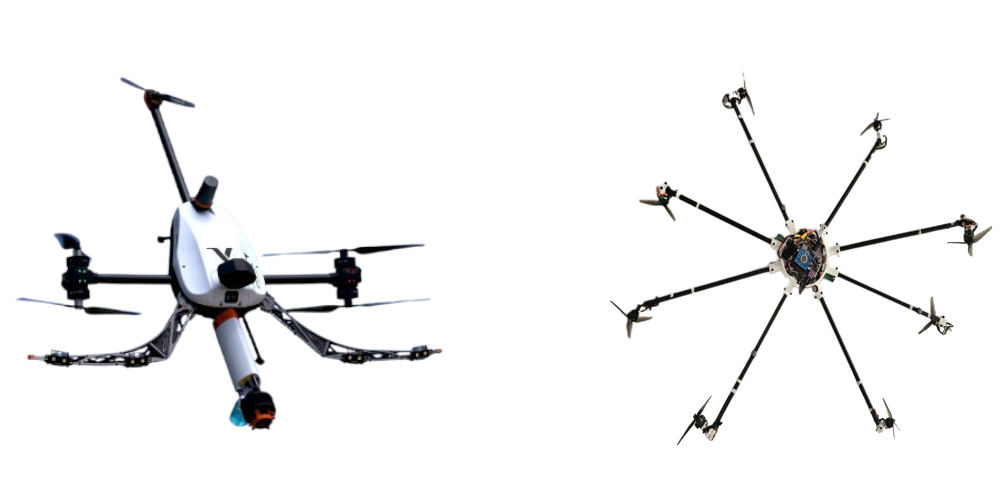
\includegraphics[width=.8\columnwidth]{figures/example_omnidirecitonal_wobg.png}
    \caption{One application of our strategy is the control of omnidirectional drones, like (left) a Voliro drone (image taken from \url{https://voliro.com}) and (right) the design from \citet{HamandiOmni}. Since they accept arbitrary $6$ DoF twists, our methodology can be used to control them to track arbitrary differentiable paths in $\text{SE}(3)$.}
    \label{fig:omnidirectionaldrone}
\end{figure}
One particularly compelling application of extending vector fields to matrix Lie groups is the control of systems capable of simultaneous motion in both position and orientation, which can be addressed by considering the group $\text{SE}(3)$ within our framework. Omnidirectional unmanned aerial vehicles (UAVs), such as those illustrated in \cref{fig:omnidirectionaldrone}, exemplify such capabilities, and research in this domain is rapidly advancing \citep{kamel2018voliro,Aboudorra2023,HamandiOmni}. For instance, \citet{hamandi2021design} provide a comprehensive review of multirotor designs, identifying critical factors that enable omnidirectional motion. These capabilities are particularly relevant for tasks requiring complex maneuvers, such as tracking paths that involve intricate trajectories. This is especially important when UAVs are equipped with tools like drills, where precise positioning is needed to achieve target poses while avoiding environmental collisions. Our approach facilitates such tasks by controlling the linear and angular velocities of the UAV. Additionally, another notable application of $\text{SE}(3)$ is in robotic manipulators, where our method can control the end effector's linear and angular velocities.

Although these applications demonstrate the versatility of our approach, it is important to emphasize that our primary focus is not on specific use cases but on the theoretical foundation itself. As will become evident, our generalization not only enables the use of vector fields on Lie groups but also reveals that the vector field strategy in Euclidean space offers more flexibility than previously recognized. To encapsulate our intent, we draw on the perspective of \citet{Bullo2004}, who states that ``the areas of overlap between mechanics and control possess the sort of mathematical elegance that makesthem appealing to study, independently of applications.''.

To illustrate the potential of our generalization, we provide two application scenarios. The first is a kinematic control simulation of a system in $\text{SE}(3)$, where the goal is to converge to and circulate along a predefined curve within the group. This simulation offers a concrete example of how our theoretical results can be practically applied and visualized. The second scenario involves a collaborative simulation in which six agents manipulate a cylindrical object with unknown properties to track a target curve. In this case, we work within the group $\mathbb{R}^3\times\text{SO}(3)$, where translation and rotation are treated as independent motions. Due to the object's unknown parameters, we employ an adaptive control strategy to estimate these properties and achieve control. Here, our vector field strategy serves as a higher-level controller, providing desired velocity inputs to a lower-level dynamic controller responsible for tracking these velocities. This simulation highlights the adaptability of our approach to dynamic scenarios, particularly those requiring parameter estimation and adaptation.

Although it does not directly enhance the understanding of this work, we include a disclaimer to address a potential question: ``Why does this work involve adaptive control if the main focus is kinematic control?'' This project originated from an effort to explore the possibilities afforded by knowledge gained during graduate courses, particularly in dynamic control using nonlinear techniques. The goal was to extend the concepts developed in course assignments to a more advanced framework. During this process, we came across an intriguing paper \citep{Culbertson2021} that tackled an adaptation problem for trajectory tracking for a manipulated body. Since their work focused on trajectory tracking, the natural question arose: ``Can we adapt this to a vector field approach, thereby shifting from trajectory tracking to path following?'' As will be shown in this text, the answer turned out to be positive.

At this point, two directions presented themselves: (1) delve further into dynamic adaptive control or (2) expand the kinematic control framework by generalizing the vector field approach. We opted for the second, as it aligned more closely with the author's interests and held greater potential for future research. Building on this choice, we extended the vector field approach proposed in \citet{Rezende2022} to incorporate orientations, resulting in a kinematic control strategy applicable to $\mathbb{R}^3\times\text{SO}(3)$. The first publication stemming from this effort covers the use of vector fields for path following in an adaptive control scheme and generalizes the vector field approach to $\mathbb{R}^3\times\text{SO}(3)$, as detailed in \citet{Pessoa2024}. This work's properties hinted at broader generalizations for vector field guidance, leading to a new question: ``How far can we extend this while preserving the intuitiveness of \citet{Rezende2022}?'' This inquiry drove the development of a more generalized vector field guidance strategy for systems represented as matrix Lie groups. The results of this endeavor were submitted to Automatica and are currently under review.

The previous disclaimer not only provides insight into how this work evolved but also explains certain modifications made to this text. Here, we focus on the generalized vector field approach for systems represented as matrix Lie groups, treating \citet{Pessoa2024} as an application of this broader framework. Consequently, our presentation adopts a non-chronological order. We begin with the more general case, as it offers a clearer conceptual foundation, and then demonstrate its application to specific scenarios. Some portions of the text from \citet{Pessoa2024} have been rewritten to better fit the context of this work and may differ from the original. Furthermore, this text includes the results of collaborative simulations, as presenting these after the strategy itself provides a more intuitive progression. Finally, we expand on certain derivations and proofs from both works to provide deeper insights.
\section{Summary of contributions}
The main contributions of this work can be summarized as follows:
\begin{itemize}
    \item Development of a novel vector field guidance strategy applicable to systems with an inherent matrix Lie group structure;
    \item Implementation framework for $\text{SE}(3)$ systems, providing all necessary tools for practical application of the proposed strategy;
    \item Validation through kinematic simulations in $\text{SE}(3)$, demonstrating the theoretical results and their practical implications;
    \item Design of an adaptive control strategy for collaborative simulations in $\mathbb{R}^3 \times \text{SO}(3)$, where the vector field guidance strategy generates reference velocities for dynamic control.
\end{itemize}

\textbf{TODO}
\begin{itemize}
    % \item Add explicit derivative for $\widehat{D}$;
    % \item Improve Lie group section;
    % \item Add Lie algebra section;
    % \item Rerun collaborative simulations using the modified model;
    % \item Change proposition 4.23 A,B etc. to X, Y...
    \item Run kinematic sim for other Lie group;
    % \item Add introduction and literature review;
    % \item Add introduction
    % \item Change symbols to reduce complexity;
    % \item Improve proof for the derivative of Lie group element, based on flows;
    % \item Add Flows + integral curves subsection in Lie group section;
    % \item Add fact that left-invariant vector fields form a basis;
    % \item Move definition of S map to Lie algebra section;
    \item Maybe change spheres in trajectory plots to UAV models.
    \item Add image showing the interpolated curve?
    % \item Add block diagram for adaptive control
    \item Chatgpt review (background) [vector field, kinematic, collaborative were review for submissions]
    % \item Add publications in Introduction
    % \item Add omnidirecitonal uav figure in intro
    \item Add reference to smooth distance in results
\end{itemize}
\section{Publications}
In this section we highlight the publications that culminated into the present work
\begin{itemize}
    \item \textbf{Pessoa, F. B. A.}; Pimenta, L. C. A. . Vector Field Based Adaptive Control for Collaborative Manipulation. In: \textbf{XXV Congresso Brasileiro de Automática}, 2024, Rio de Janeiro. Anais do XXV Congresso Brasileiro de Automática, 2024
    \item \textbf{Bartelt, F.}; Gonçalves, V. M.; Pimenta, L. C. A. . Constructive Vector Fields for Path Following in Matrix Lie Groups. \textbf{Submitted to Automatica}, 2025.
\end{itemize}
\section{Structure of the text}
This chapter is organized as follows:
\begin{itemize}
    \item \chapref{chap:literature-review}\\
    We review the formulation of vector fields and the application of Lie theory across various domains.
    \item \chapref{ch:background}\\
    This chapter revisits the vector field guidance strategy in Euclidean space, provides the necessary background on Lie groups and Lie algebras, and introduces the foundational concepts of adaptive control.
    \item \chapref{ch:vector_field}\\
    We present the generalization of the vector field guidance strategy to matrix Lie groups.
    \item \chapref{ch:kinematic}\\
    We detail the application of the strategy to kinematic control in exponential Lie groups and provide the tools required for implementation in $\text{SE}(3)$.
    \item \chapref{ch:collaborative}\\
    This chapter introduces the system model, the lower-level controller, and the adaptive control strategy for a collaborative manipulation scenario.
    \item \chapref{ch:results}\\
    We present the details and results of simulations for both explored scenarios.
    \item \chapref{ch:conclusion}\\
    The text concludes with a summary of the findings and a discussion of potential directions for future research.
\end{itemize}


% !TeX root = main.tex
\chapter{Thoeretical Background}\label{ch:background}
In this chapter we revisit the vector field strategy in the euclidean space based on a curve parametrization \citep{Rezende2022}, as it will prove valuable in drawing connections between both works. We also present some fundamental concepts of Lie groups and Lie algebras, which will be essential for the development of our extension.

\section{Vector Field in Euclidean Space}\label{sec:adriano-review}
For clarity, we revisit the vector field strategy presented in \citet{Rezende2022}. Since our work extends this previous approach, this review will help establish direct connections between both works and highlight the core aspects of our contributions. The primary goal of the authors in \citet{Rezende2022} is to develop an artificial $n$-dimensional vector field that guides system trajectories toward a predefined curve and ensures circulation around it. A key element of this formulation is the definition of a distance function with essential properties. As their work focuses solely on Euclidean space, they adopt the Euclidean distance for the vector field computation, which is derived using a parametric representation of the curve.

We summarize the main steps for constructing this vector field, emphasizing the most critical properties. Although the original paper addresses time-varying curves, we limit our discussion to the static portion of the methodology. The authors consider a system modeled as the following single integrator 
\begin{align}
    \dot{\mathbf{h}} = \boldsymbol{\xi}, \label{eq:adriano-single-integrator}
\end{align}
where $\mathbf{h}\in\mathbb{R}^m$ represents the system state, and $\boldsymbol{\xi}\in\mathbb{R}^m$ denotes the system input. The objective is to compute a vector field $\Psi:\mathbb{R}^m\to\mathbb{R}^m$ such that, if the system input is equal to the vector field, the system trajectories converge to and follow the target curve $\mathcal{C}$, for which a parametrization is given by $\mathbf{h}_d(s)$. Despite relying on a parametric representation of the curve, it is important to note that the resulting computations are independent of the specific parametrization chosen.

The authors define their distance function $D$ as the Euclidean distance between the system's current state and the nearest point on the curve, i.e., 
\begin{align}
    D(\mathbf{h}) \triangleq \min_{s}\widehat{D}(\mathbf{h}, \mathbf{h}_d(s))=\min_{s}\|\mathbf{h}- \mathbf{h}_d(s)\|. \label{eq:adriano-EC-distance}   
\end{align}
In this context, we denote $s^*$ as the optimal parameter such that $\mathbf{h}_d(s^*(\mathbf{h}))$ is the closest point on the curve to the current state.
\begin{figure}
    \centering
    \def\svgwidth{.8\linewidth}
    \import{figures/}{plotly_vf2.pdf_tex}
    \caption{Example showing the vector field and the components for a point $\mathbf{h}\in G$ and curve $\mathcal{C}$.}
    \label{fig:vector-field-adriano}
\end{figure}

Next, the authors introduce two components of their vector field: the \emph{normal} component $\boldsymbol{\xi}_{N}$, responsible for convergence, and the \emph{tangent} component $\boldsymbol{\xi}_{T}$, which ensures circulation. The resulting expression for the vector field is 
\begin{align}
    \Psi(\mathbf{h}) = k_N(\mathbf{h})\boldsymbol{\xi}_{N}(\mathbf{h}) + k_T(\mathbf{h})\boldsymbol{\xi}_{T}(\mathbf{h}), \label{eq:adriano-vector-field-expression}    
\end{align}
where $k_N$ and $k_T$ are gains, dependent on the system state, that balance the predominance of the normal and tangent components. This vector field strategy is illustrated in \autoref{fig:vector-field-adriano}. The normal component, $\boldsymbol{\xi}_{N}$, is naturally taken as the negative gradient of the distance function, due to the use of Euclidean distance:
\begin{align}
    \boldsymbol{\xi}_{N} = -\nabla D.
\end{align}

There is a key aspect of the normal component that is crucial for the convergence proof using Lyapunov stability theory: the fact that the time derivative of the distance function can be expressed as $\dot{D}=-\boldsymbol{\xi}_{N}^{\top}{\boldsymbol{\xi}}$. We emphasize the significance of this feature, as it will play an important role in our extension. In our approach, the normal component is similarly constructed by identifying the term that arises when differentiating the distance function.

Next, we address the tangent component. This component is solely related to the target curve and is defined as the tangent vector at the nearest point on the curve, i.e.,
\begin{align}
    \boldsymbol{\xi}_{T}(\mathbf{h}) = \frac{d}{ds}\mathbf{h}_d(s)|_{s=s^*(\mathbf{h})}.
\end{align}
A noteworthy property of both components is that they are orthogonal to each other, which is essential in the proof of convergence for this algorithm.

In the Lyapunov stability proof, the final result shows that the time derivative of $D$ is negative semidefinite. The proof is then completed using two other essential properties: the fact that the distance function has no local minima outside the curve, and the fact that the ``generalized gradient'' of this function never vanishes. With these features, the authors demonstrate that if the system trajectories follow the vector field, the system will converge to and circulate around a predefined curve. A summary of these key features is as follows:
\begin{feature}
    \item The time derivative of the distance function is the opposite of the dot product between the so called \emph{normal} component and the system control input; \label{feat:adriano-time-derivative-lyapunov-normal-comp}
    \item The \emph{normal} and \emph{tangent} components are orthogonal to each other; \label{feat:adriano-orthogonality}
    \item The distance function has no local minima outside the target curve. Furthermore, whenever the distance function is differentiable, its gradient never vanishes. \label{feat:adriano-no-local-minima}
\end{feature}
In our generalization, we will incorporate and build upon these features.

\section{Lie groups and Lie algebras}\label{sec:background-lie-theory}
In this section, we introduce \emph{Lie groups}, which are smooth manifolds that are also groups, and \emph{Lie algebras}. Besides providing examples of both, we also introduce concepts that will prove valuable in our work. This section integrates concepts and ideas from the following books: \citet{Lee2012,Gallier2020,Hall2015,Duistermaat2012}, with the aim of presenting the concepts in a clearer and more accessible manner. We begin with the general definition of a Lie group.
\subsection{Lie groups}
\begin{definition}[Lie group]
    A \emph{Lie group} is a smooth manifold $G$ satisfying the following properties:
    \begin{property}
        \item $G$ is a group (with identity element denoted $\iota$)
        \item $G$ is a topological group (the group operation and the inverse map are continuous). Furthermore, the group operation $\circ: G\times G\to G$ and the inverse map $\cdot^{-1}: G\to G$ are smooth.
    \end{property}
\end{definition}

The mapping between Lie groups is a fundamental concept and will play an important role in our extension, specifically for drawing connections between our extension and the vector field strategy in Euclidean space. Usually these mappings have additional properties and are defined as follows:
\begin{definition}
    If $G$ and $H$ are Lie groups, a \emph{homomorphism} $\mathcal{H}: G\to H$ is a smooth map (between manifolds $G$ and $H$) that is also a group homomorphism, that is, if $\circ$ and $\star$ are the group operations in $G$ and $H$, respectively, then $\mathcal{H}(\mathbf{X}\circ\mathbf{Y}) = \mathcal{H}(\mathbf{X})\star\mathcal{H}(\mathbf{Y})$ for all $\mathbf{X},\mathbf{Y}\in G$. If this map is also a diffeomorphism (the inverse map $\mathcal{H}^{-1}$ is also a homomorphism), then $\mathcal{H}$ is an \emph{isomorphism}. In this case, we say that $G$ and $H$ are \emph{isomorphic} and denote this by $G\cong H$.
\end{definition}

There are two important isomorphisms in Lie groups that are important for the concept of Lie algebras. These are the translation isomorphisms, which are defined as follows:
\begin{definition}
    Given a Lie group $G$, we define two operations: the left translation $\mathcal{L}_{\mathbf{X}}: G\to G$ and the right translation $\mathcal{R}_{\mathbf{X}}: G\to G$ for any $\mathbf{X}\in G$. These operations are defined as 
    \begin{align}
        \mathcal{L}_{\mathbf{X}}(\mathbf{Y}) &= \mathbf{X}\circ\mathbf{Y}\\
        \mathcal{R}_{\mathbf{X}}(\mathbf{Y}) &= \mathbf{Y}\circ\mathbf{X},
    \end{align}
    respectively. Since the group operation and the inverse map are smooth, the left and right translations are diffeomorphisms, and thus isomorphisms.
\end{definition}

\subsubsection{Matrix Lie Groups}
In general lines, Lie groups that can be represented by matrices are called \emph{matrix Lie groups}. These groups are defined by a set of matrices that satisfy the group properties. The group operation is matrix multiplication, the identity element is the identity matrix, and the inverse map is the matrix inverse. For a more precise definition, we need to define the \emph{general linear group} and the concept of \emph{convergence} of a sequence of matrices.
\begin{definition}
    The \emph{general linear group} over the real numbers, denoted $\text{GL}(n, \mathbb{R})$, is the set of all invertible $n\times n$ matrices with real entries. The general linaer group over the complex numbers, denoted $\text{GL}(n, \mathbb{C})$, is the group of all invertible $n\times n$ matrices with complex entries.
\end{definition}
\begin{definition}
    Let $\mathbf{X}_k$ be a sequence of complex matrices in $\mathbb{C}^{n\times n}$. We say that $\mathbf{X}_k$ \emph{converges} to a matrix $\mathbf{Y}$ if each entry of $\mathbf{X}_k$ converges to the corresponding entry of $\mathbf{Y}$ as $k\to\infty$. This means that for each $i,j\in[1,n]$, the sequence $\{\mathbf{X}_k\}_{ij}$ converges to $\mathbf{Y}_{ij}$.
\end{definition}
With both definitions, we can now define a matrix Lie group formally.
\begin{definition}
    A \emph{matrix Lie group} is a subgroup $G$ of $\text{GL}(n, \mathbb{C})$ with the property that if $\mathbf{X}_k$ is a sequence of matrices in $G$, and $\mathbf{X}_k$ converges to some matrix $\mathbf{Y}$, then either $\mathbf{Y}$ is in $G$ or $\mathbf{Y}$ is not invertible. This property is equivalent to sayint that $G$ is a \emph{closed subgroup} of $\text{GL}(n, \mathbb{C})$.
\end{definition}

Although present in the context of any Lie group, we can define two interesting properties more easily for matrix Lie groups. The knowledge of \emph{compactness} and \emph{connectedness} can reduce complexity in the study of these groups.
\begin{definition}
    A matrix Lie group $G\subset\text{GL}(n,\mathbb{C})$ is said to be \emph{compact} if and only if:
    \begin{property}
        \item whenever a sequence $\mathbf{X}_k$ is in $G$ and $\mathbf{X}_k$ converges to $\mathbf{Y}$, then $\mathbf{Y}$ is in $G$;
        \item there exists a constant $C>0$ such that for all $\mathbf{X}\in G$, $\|\{\mathbf{X}\}_{ij}\|\leq C$ for all $i,j\in[1,n]$.
    \end{property}
\end{definition}
\begin{definition}
    A matrix Lie group $G$ is termed \emph{connected} if for all $\mathbf{X},\mathbf{Y}\in G$, there exists a continuous path $\mathbf{G}(\sigma)\in G$, $a\le\sigma\le b$ such that $\mathbf{G}(a) = \mathbf{X}$ and $\mathbf{G}(b) = \mathbf{Y}$. The \emph{identity component} of $G$, denoted $G_\iota$, is the set $\mathbf{X}\in G$ for which there exists a continuous path $\mathbf{G}(\sigma)\in G$, $a\le\sigma\le b$ such that $\mathbf{G}(a) = \iota=\mathbf{I}$ and $\mathbf{G}(b) = \mathbf{X}$.
\end{definition}

\subsubsection{Examples of Lie groups}
In this section we present some examples of the most common Lie groups, which will also introduce the notation and concepts that will be used in our extension.
\begin{example}\label{ex:general-linear-group-special-linear-group}
    The \emph{special linear group} $\text{SL}(n, \mathbb{R})$ (resp. $\text{SL}(n, \mathbb{C})$) is a subgroup of $\text{GL}(n, \mathbb{R})$ (resp. $\text{GL}(n, \mathbb{C})$) consisting of invertible matrices with determinant equal to 1.
\end{example}
\begin{example}
    The group formed by the direct product of Lie groups $G = G_1 \times G_2 \times \dots \times G_k$ is a Lie group \citep[p. 152]{Lee2012}. It is also true that the semidirect product of Lie groups $G = G_1\rtimes G_2$ is also a Lie group \citep[p. 168]{Lee2012}.
\end{example}
\begin{example}\label{ex:orthogonal-group-special-orthogonal-group}
    The \emph{orthogonal group} $\text{O}(n)$ is the Lie group of distance-preserving transformation and comprises rotations and reflections. It consists of all $n\times n$ orthogonal matrices:
    \begin{align}
        \text{O}(n) = \left\{\mathbf{X}\in\mathbb{R}^{n\times n} | \mathbf{X}^T\mathbf{X} = \mathbf{I}_n\right\}.
    \end{align}

    Its subgroup $\text{SO}(n)$, the \emph{special orthogonal group}, consists of all orthogonal matrices with determinant equal to 1. This group represents rotations and as such are formed by the set of rotation matrices:
    \begin{align}
        \text{SO}(n) = \left\{\mathbf{X}\in\mathbb{R}^{n\times n} | \mathbf{X}^T\mathbf{X} = \mathbf{I}_n,\, \det(\mathbf{X}) = 1\right\}.
    \end{align}
\end{example}
\begin{example}\label{ex:euclidean-group-special-euclidean-group}
    The \emph{Euclidean group} $\text{E}(n)$ is a Lie group of isometries in Euclidean space. This group is formed by the semidirect product $\mathbb{R}^n \rtimes \text{O}(n)$ and is defined as
    \begin{align}
        \text{E}(n) = \left\{\begin{bmatrix}
            \mathbf{R} & \mathbf{p} \\ \mathbf{0} & 1
        \end{bmatrix} \in \mathbb{R}^{(n+1)\times(n+1)} | \mathbf{R}\in\text{O}(n),\, \mathbf{p}\in\mathbb{R}^n\right\}.
    \end{align}

    Its subgroup $\text{SE}(n)$, the \emph{special Euclidean group}, consists of all matrices in the Euclidean group with determinant equal to 1, formed by the semidirect product $\mathbb{R}^n\rtimes \text{SO}(n)$. This group represents rigid transformations and is formed by the set of homogeneous transformation matrices:
    \begin{align}
        \text{SE}(n) = \left\{\begin{bmatrix}
            \mathbf{R} & \mathbf{p} \\ \mathbf{0} & 1
        \end{bmatrix} \in \mathbb{R}^{(n+1)\times(n+1)} | \mathbf{R}\in\text{SO}(n),\, \mathbf{p}\in\mathbb{R}^n\right\}.
    \end{align}
\end{example}
\begin{example}\label{ex:translation-group}
    The group $(\mathbb{R}^n,+)$, also denoted $\mathbb{R}^n$, is also a Lie group, where the group operation is the vector addition, the identity element is the zero vector, and the inverse map is the negation of the vector. We will usually represent this group through an inclusion map $\mathbb{R}^n \hookrightarrow \text{SE}(n)$ and denote the group under this inclusion the \emph{translation group} $\text{T}(n)$, defined as
    \begin{align}
        \text{T}(n) = \left\{\begin{bmatrix}
            \mathbf{I}_n & \mathbf{p} \\ \mathbf{0} & 1
        \end{bmatrix} \in \text{SE}(n) | \mathbf{p}\in\mathbb{R}^n\right\}.
    \end{align}
\end{example}
\begin{example}\label{ex:independent-translation-rotation-ISE}
    Although not present in the literature, we introduce the group of independent translations and rotations (\emph{Independent Special Euclidean group}) $\text{ISE}(n)\cong\mathbb{R}^n\times\text{SO}(n)$, defined as
    \begin{align}
        \begin{split}
            \text{ISE}(n) &= \left\{\begin{bmatrix}
            \mathbf{R} & \mathbf{0}\\
            \mathbf{0} & \mathbf{P}\\
            \end{bmatrix}\in\mathbb{R}^{(2n+1)\times(2n+1)}\,|\, \mathbf{R}\in\text{SO}(n),\,\mathbf{P}\in\text{T}(n)\right\}\\
            &= \left\{\begin{bmatrix}
            \mathbf{R} & \mathbf{0} & \mathbf{0}\\
            \mathbf{0} & \mathbf{I} & \mathbf{p}\\
            \mathbf{0} & \mathbf{0} & 1
            \end{bmatrix}\in\mathbb{R}^{(2n+1)\times(2n+1)}\,|\, \mathbf{R}\in\text{SO}(n),\,\mathbf{p}\in\mathbb{R}^n\right\}.
        \end{split} \label{eq:ISE-group}
    \end{align}
    Although they are isomorphic, we will use the representation $\mathbb{R}^n\times \text{SO}(n)$ to denote tuples of translations and rotations $(\mathbf{p},\mathbf{R})$, and the representation $\text{ISE}(n)$ to denote elements represented as the matrices in \eqref{eq:ISE-group}. Note that we can use both representations interchangeably, since we can easily extract the position and orientation from the matrix representation by means of matrix multiplication.
\end{example}
\begin{example}\label{ex:symplectic-group}
    The \emph{real symplectic group} $\text{Sp}(2n)$ is the group of all $2n\times 2n$ real matrices that preserve a non-degenerate skew-symmetric bilinear form $\omega$. This group plays an important role in classical mechanics, specially in the study of Hamiltonian systems. The group is defined as
    \begin{align}
        \text{Sp}(2n) &= \left\{\mathbf{X}\in\mathbb{R}^{2n\times 2n} | \mathbf{X}^\top\boldsymbol{\Omega}\mathbf{X} = \boldsymbol{\Omega}\right\}\\
        &= \left\{\mathbf{X}\in\mathbb{R}^{2n\times 2n} | -\boldsymbol{\Omega}\mathbf{X}^\top\boldsymbol{\Omega} = \mathbf{X}^{-1}\right\},
    \end{align}
    where 
    \begin{align}
        \boldsymbol{\Omega} = \begin{bmatrix}
            \mathbf{0} & \mathbf{I}_n\\
            -\mathbf{I}_n & \mathbf{0}
        \end{bmatrix}.
    \end{align}
    The skew-symmetric bilinear form can be characterized by $\omega(x,y)=\langle x, \boldsymbol{\Omega}y\rangle\,\forall\,x,y\in\mathbb{R}^{2n}$. We can also define the \emph{complex symplectic group} $\text{Sp}(2n, \mathbb{C})$ as the group of all $n\times n$ complex matrices that preserve the same non-degenerate skew-symmetric bilinear form, thus the group definition is the same, but with matrices with complex entries.
\end{example}
\begin{example}
    The \emph{indefinite orthogonal group} (or generalized orthogonal group) $\text{O}(p,q)$ is the group of all $n\times n$ real matrices
    \begin{align}
        \text{O}(p,q) = \left\{\mathbf{X}\in\mathbb{R}^{n\times n} | \mathbf{X}^\top\mathbf{I}_{p,q}\mathbf{X} = \mathbf{I}_{p,q}\right\},
    \end{align}
    where
    \begin{align}
        \mathbf{I}_{p,q} = \begin{bmatrix}
            \mathbf{I}_p & \mathbf{0}\\
            \mathbf{0} & -\mathbf{I}_q
        \end{bmatrix},
    \end{align}
    and $n=p+q$.

    Similarly, we can define the \emph{indefinite special orthogonal group} $\text{SO}(p,q)$ as the group
    \begin{align}
        \text{SO}(p, q) = \left\{\mathbf{X}\in\text{O}(p, q) | \det\mathbf{X}=1\right\}.
    \end{align}
    The group $\text{O}(1,3)$ is of particular interest in the study of special relativity, and is denoted the \emph{Lorentz group}. This group preserves the Lorentz metric
    \begin{align}
        (t,x,y,z) \mapsto t^2 - x^2 - y^2 - z^2.
    \end{align}
    The Lorentz group is also represented as $\text{O}(3,1)$, which would preserve the metric $x^2 + y^2 + z^2 - t^2$.
    If we restrict this group to transformations that preserve orientation, we obtain the \emph{proper Lorentz group} $\text{SO}(1,3)$. Furthermore, the subgrtoup of all Lorentz transformations that preserve orientation and the time direction is called the  \emph{proper orthochronous Lorentz group} $\text{SO}^+(1,3)$, this is the identity component $G_\iota$ of $\text{SO}(1,3)$.
    
\end{example}
% ADD Examples for indefinite orthogonal (with lorentz), heisenberg?, and symplectic groups
\begin{example}\label{ex:non-matrix-lie-group}
    An example of a Lie group that is not a matrix Lie group is given in \citet[p. 25]{Hall2015} and reproduced here:

    The group $G = \mathbb{R} \times \mathbb{R} \times \mathbb{S}^1 = \left\{(x, y, \theta) | x \in \mathbb{R}, y \in \mathbb{R}, \theta \in \mathbb{S}^1\subset\mathbb{C}\right\}$, equipped with the group operation
    \begin{align}
        (x_1, y_1, \theta_1)\circ (x_2, y_2, \theta_2) = (x_1 + x_2, y_1 + y_2, e^{ix_1y_2}\theta_1\theta_2),
    \end{align}
    is a Lie group without a matrix representation. The identity element is $\iota=(0, 0, 1)$, and the inverse map is $(x, y, \theta)^{-1} = (-x, -y, e^{ixy}\theta^{-1})$.
\end{example} 

\subsection{Lie algebras}
Lie groups are closely associated with a mathematical structure called the \emph{Lie algebra}, which allows us to study their properties using linear algebra. Usually the Lie algebra of a Lie group $G$ is denoted as the set of all smooth \emph{left-invariant} vector fields on $G$, denoted $\text{Lie}(G)$. These are vector fields that remain unchanged when ``shifted'' by the group operations. To define left-invariant vector fields formally, we first need to understand the concept of differentials in the context of Lie groups.

Suppose $\mathcal{H}:G\to H$ is a homomorphism between Lie groups $G$ and $H$. If $V$ is a vector field on $G$, then at every point $\mathbf{X}\in G$, the differential of $\mathcal{H}$ at $\mathbf{X}$, denoted $d(\mathcal{H})_\mathbf{X}$, maps the vector $V(\mathbf{X})$ in the tangent space of $G$ at $\mathbf{X}$ to a vector in the tangent space of $H$ at $\mathcal{H}(\mathbf{X})$, i.e. $d(\mathcal{H})_\mathbf{X}:T_\mathbf{X}G\to T_{\mathcal{H}(\mathbf{X})}H$.

Furthermore, if there exists a vector field $W$ on $H$ such that $d(\mathcal{H})_\mathbf{X}\bigl(V(\mathbf{X})\bigr) = W\bigl(\mathcal{H}(\mathbf{X})\bigr)$ for all $\mathbf{X}\in G$, then $V$ and $W$ are said to be $\mathcal{H}$-related. This concept is important since if $\mathcal{H}$ is a diffeomorphism, a Lie group isomorphism in this context, then there is a unique vector field $W$ on $H$ that is $\mathcal{H}$-related to $V$ \citep[p. 183]{Lee2012}.

Finally, the concept of left-invariant (resp. right-invariant) vector fields on Lie groups can be introduced by means of the differential mappings of these translations:
\begin{definition}
    A vector field $V$ on a Lie group $G$ is said to be \emph{left-invariant} (resp. \emph{right-invariant}) if it is invariant under all left (resp. right) translations:
    \begin{align*}
        d(\mathcal{L}_\mathbf{X})_\mathbf{Y}(V(\mathbf{Y})) &= V(\mathbf{X}\circ\mathbf{Y}) \,\forall\,\mathbf{X},\mathbf{Y}\in G,\\
        \text{(resp.) }d(\mathcal{R}_\mathbf{X})_\mathbf{Y}(V(\mathbf{Y})) &= V(\mathbf{Y}\circ\mathbf{X}) \,\forall\,\mathbf{X},\mathbf{Y}\in G.
    \end{align*}  
\end{definition}
Since the translation operations are isomorphisms, it follows that every left-invariant (resp. right-invariant) vector field on a Lie group can be identified with its value at the identity element. In other words, if $V$ is a left-invariant (resp. right-invariant) vector field and $V_\iota\triangleq V(\iota) \in T_\iota G$ is the value of the vector field at the identity element of $G$, then $V$ and $V_\iota$ are $\mathcal{L}_\mathbf{X}$-related (resp. $\mathcal{R}_\mathbf{X}$-related) for all $\mathbf{X}\in G$, which implies that $V(\mathbf{X}) = d(\mathcal{L}_\mathbf{X})_\iota V_\iota$ (resp. $V(\mathbf{X}) = d(\mathcal{R}_\mathbf{X})_\iota V_\iota$).

From the last statement, it is clear that the Lie algebra is a vector space that captures the local behavior of the group around the identity element. For this reason, the Lie algebra of a Lie group $G$ is also defined as the tangent space at the identity element $T_\iota G$, commonly denoted $\mathfrak{g}$. More generally, a Lie algebra is defined as follows:
\begin{definition}
    A \emph{real Lie algebra} is a real vector space $\mathfrak{g}$, endowed with a map $[\cdot, \cdot]:\mathfrak{g}\times\mathfrak{g}\to\mathfrak{g}$, called the \emph{Lie bracket} on $\mathfrak{g}$, that satisfies the following properties for all $\mathbf{A},\mathbf{B},\mathbf{C}\in\mathfrak{g}$:
    \begin{property}
        \item \emph{Bilinearity}: For all $a,b\in\mathbb{R}$,
        \begin{align*}
            [a\mathbf{A}+b\mathbf{B}, \mathbf{C}] &= a[\mathbf{A}, \mathbf{C}] + b[\mathbf{B}, \mathbf{C}], \\
             [\mathbf{C}, a\mathbf{A}+b\mathbf{B}] &= a[\mathbf{C}, \mathbf{A}] + b[\mathbf{C}, \mathbf{B}];
        \end{align*}
        \item \emph{skew-symmetry}: 
        \begin{align*}
            [\mathbf{A}, \mathbf{B}] = -[\mathbf{B}, \mathbf{A}];
        \end{align*} \label{prop:lie-algebra-skew-symmetry}
        \item \emph{Jacobi identity}:
        \begin{align*}
            [\mathbf{A}, [\mathbf{B}, \mathbf{C}]] + [\mathbf{B}, [\mathbf{C}, \mathbf{A}]] + [\mathbf{C}, [\mathbf{A}, \mathbf{B}]] = 0.
        \end{align*}
    \end{property}
\end{definition}
Note that \cref{prop:lie-algebra-skew-symmetry} implies that $[\mathbf{A}, \mathbf{A}]=0\,\forall\,\mathbf{A}\in\mathfrak{g}$. 

Mappings between Lie algebras also have an important role in the study of Lie groups, specially homomorphisms and isomorphisms. The definition of a homomorphism between Lie algebras is given as follows:
\begin{definition}
    If $\mathfrak{g}$ and $\mathfrak{h}$ are Lie algebras with Lie brackets $[\cdot, \cdot]_\mathfrak{g}$ and $[\cdot, \cdot]_\mathfrak{h}$, respectively, a linear map $\mathscr{H}:\mathfrak{g}\to\mathfrak{h}$ is denoted a \emph{homomorphism} if it preserves the Lie bracket, that is, $\mathscr{H}([\mathbf{A}, \mathbf{B}]_\mathfrak{g}) = [\mathscr{H}(\mathbf{A}), \mathscr{H}(\mathbf{B})]_\mathfrak{h}\,\forall\, \mathbf{A},\mathbf{B}\in\mathfrak{g}$. Furthermore, if $\mathscr{H}$ is a bijection, then $\mathscr{H}^{-1}$ is also a homomorphism, and $\mathscr{H}$ is an \emph{isomorphism}. In this case, we say that $\mathfrak{g}$ and $\mathfrak{h}$ are \emph{isomorphic} and denote this by $\mathfrak{g}\cong\mathfrak{h}$.
\end{definition}
Lie algebra homomorphisms can also be induced by Lie group homomorphisms. If $\mathcal{H}$ is a Lie group homomorphism between Lie groups $G$ and $H$, then the differential of $\mathcal{H}$ at the identity element $d\mathcal{H}_\iota=\mathscr{H}$ is a Lie algebra homomorphism between the Lie algebras $\mathfrak{g}=T_\iota G$ and $\mathfrak{h}=T_\iota H$ \citep[p. 41]{Duistermaat2012}. Furthermore, if $\mathcal{H}$ is a Lie group isomorphism, then $d\mathcal{H}_\iota$ is a Lie algebra isomorphism.

The most important Lie algebra homomorphism is the differential of the translation operations. As previously seem, every left-invariant (resp. right-invariant) vector field can be identified with the tangent space at the identity element, and since the translation operations are isomorphisms, the space of left-invariant (resp. right-invariant) vector fields $\text{Lie}(G)$ is isomorphic to the tangent space at the identity element $\mathfrak{g}$, i.e. $\text{Lie}(G)\cong\mathfrak{g}$. Both definitions of the Lie algebra of a Lie group are equally important and are used interchangeably depending on the context, as one definition might allow for easier comprehension or computtions. The concept of homomorphisms thus tie both definitions together.
\subsubsection{Examples of Lie algebras}
In this section we present the corresponding ones for the Lie groups presented in the previous section, as well as some Lie algebras isomorphisms.
\begin{example}
    The Lie algebra of the general linear group $\text{GL}(n, \mathbb{R})$ is the set of all $n\times n$ matrices, denoted $\mathfrak{gl}(n, \mathbb{R})$, with its Lie bracket given by the commutator $[\mathbf{A}, \mathbf{B}] = \mathbf{A}\mathbf{B} - \mathbf{B}\mathbf{A}$. Similarly, the Lie algebra of the general linear group $\text{GL}(n, \mathbb{C})$, denoted $\mathfrak{gl}(n, \mathbb{C})$, is the set of all $n\times n$ complex matrices with the same Lie bracket. Furthermore, the Lie algebra of the special linear group $\text{SL}(n, \mathbb{R})$ (resp. $\text{SL}(n, \mathbb{C})$) is the set of all $n\times n$ real (resp. complex) matrices with zero trace, denoted $\mathfrak{sl}(n, \mathbb{R})$ (resp. $\mathfrak{sl}(n, \mathbb{C})$).
\end{example}
\begin{example}
    The lie algebra for the direct product of Lie groups $G=G_1 \times G_2 \times \dots \times G_k$ is the direct sum of the Lie algebras of the groups, i.e. $\mathfrak{g}_1\oplus\mathfrak{g}_2\oplus\dots\oplus\mathfrak{g}_k$.
\end{example}
\begin{example}
    The Lie algebra of the orthogonal group $\text{O}(n)$ is the same as the Lie algebra of the special orthogonal group $\text{SO}(n)$, denoted $\mathfrak{so}(n)$. This Lie algebra is the set of all $n\times n$ skew-symmetric matrices:
    \begin{align*}
        \mathfrak{so}(n) = \left\{\mathbf{A}\in\mathbb{R}^{n\times n} | \mathbf{A}^\top = -\mathbf{A}\right\}.
    \end{align*}
    In the special case of the special orthogonal Lie group $\text{SO}(3)$, with Lie algebra $\mathfrak{so}(3)$, a common basis is given by the of matrices
    \begin{align*}
        \mathbf{E}_1 = \begin{bmatrix} 0 & 0 & 0 \\ 0 & 0 & -1 \\ 0 & 1 & 0 \end{bmatrix}, \quad \mathbf{E}_2 = \begin{bmatrix} 0 & 0 & 1 \\ 0 & 0 & 0 \\ -1 & 0 & 0 \end{bmatrix}, \quad \mathbf{E}_3 = \begin{bmatrix} 0 & -1 & 0 \\ 1 & 0 & 0 \\ 0 & 0 & 0 \end{bmatrix}.
    \end{align*}
    It is usual to represent elements of $\mathfrak{so}(3)$ through a map $\SL$ that maps a vector $\boldsymbol{\zeta} = [\zeta_1\ \zeta_2\ \zeta_3]^\top$ into a skew-symmetric matrix:
    \begin{align*}
        \SL[\boldsymbol{\zeta}] = \zeta_1 \mathbf{E}_1 + \zeta_2 \mathbf{E}_2 + \zeta_3 \mathbf{E}_3
        = \begin{bmatrix} 0 & -\zeta_3 & \zeta_2 \\ \zeta_3 & 0 & -\zeta_1 \\ -\zeta_2 & \zeta_1 & 0 \end{bmatrix}.
    \end{align*}
    In fact, this map is an isomorphism between the Lie algebra of $\mathbb{R}^3$ and $\mathfrak{so}(3)$. Let the Lie bracket of $\mathbb{R}^3$ be the cross product, $\mathbf{a} = [a_1\ a_2\ a_3]^\top$ and $\mathbf{b} = [b_1\ b_2\ b_3]^\top$, then 
    \begin{align*}
        \SL[\mathbf{a}\times \mathbf{b}] &= \begin{bmatrix}
            0 & a_2b_1-a_1b_2 & a_3b_1-a_1b_3\\
            a_1b_2 - a_2b_1 & 0 & a_3b_2-a_2b_3\\
            a_1b_3-a_3b_1 & a_2b_3-a_3b_2 & 0
        \end{bmatrix},
    \end{align*}
    now computing $\SL[\mathbf{a}]\SL[\mathbf{b}]$ and $\SL[\mathbf{b}]\SL[\mathbf{a}]$ gives
    \begin{align*}
        \SL[\mathbf{a}]\SL[\mathbf{b}] &=
        \begin{bmatrix}
            -a_3b_3 -a_2b_2 & a_2b_1 & a_3b_1\\
            a_1b_2 & -a_3b_3 - a_1b_1 & a_3b_2\\
            a_1b_3 & a_2b_3 & -a_2b_2 - a_1b_1
        \end{bmatrix},\\
        \SL[\mathbf{b}]\SL[\mathbf{a}] &=
        \begin{bmatrix}
            -a_3b_3 -a_2b_2 & a_1b_2 & a_1b_3\\
            a_2b_1 & -a_3b_3 - a_1b_1 & a_2b_3\\
            a_3b_1 & a_3b_2 & -a_2b_2 - a_1b_1
        \end{bmatrix}.
    \end{align*}
    Clearly, $\SL[\mathbf{a}\times \mathbf{b}] = [\SL[\mathbf{a}], \SL[\mathbf{b}]] = \SL[\mathbf{a}]\SL[\mathbf{b}] - \SL[\mathbf{b}]\SL[\mathbf{a}]$, which shows that $\SL$ is an isomorphism between $\mathbb{R}^3$ and $\mathfrak{so}(3)$.
\end{example}
\begin{example}
    The Lie algebra of the Euclidean group $\text{E}(n)$ and the special Euclidean group $\text{SE}(n)$ is denoted $\mathfrak{se}(n)$, and is the set 
    \begin{align*}
        \mathfrak{se}(n) = \left\{\begin{bmatrix}
            \mathbf{A} & \mathbf{b} \\ \mathbf{0} & 0
        \end{bmatrix} \in \mathbb{R}^{(n+1)\times(n+1)} | \mathbf{A}\in\mathfrak{so}(n),\, \mathbf{b}\in\mathbb{R}^n\right\}.
    \end{align*}
    specially in the case of $\mathfrak{se}(3)$, although some texts refer to elements of the Lie algebra as twists, the most common representation is given by a six-dimensional vector, the twit, $\boldsymbol{\zeta} = [\zeta_1\ \zeta_2\ \zeta_3\ \zeta_4\ \zeta_5\ \zeta_6]^\top$ and an isomorphism $\SL$ is given by
    \begin{align*}
        \SL[\boldsymbol{\zeta}] = \begin{bmatrix}
            0 & -\zeta_6 & \zeta_5 & \zeta_1 \\
            \zeta_6 & 0 & -\zeta_4 & \zeta_2 \\
            -\zeta_5 & \zeta_4 & 0 & \zeta_3 \\
            0 & 0 & 0 & 0
        \end{bmatrix},
    \end{align*}
    where $[\zeta_1\ \zeta_2\ \zeta_3]^\top$ is the linear velocity $\mathbf{v}$ and $[\zeta_4\ \zeta_5\ \zeta_6]^\top$ is the angular velocity $\boldsymbol{\omega}$.
\end{example}
\begin{example}
    The Lie algebra of $\text{T}(n)$ is a subset of $\mathfrak{se}(n)$, and is given by
    \begin{align*}
        \mathfrak{t}(n) = \left\{\begin{bmatrix}
            \mathbf{0} & \mathbf{a} \\ \mathbf{0} & 0
        \end{bmatrix} \in \mathfrak{se}(n) | \mathbf{a}\in\mathbb{R}^n\right\}.
    \end{align*} 
\end{example}
\begin{example}
    The Lie algebra of the independent special Euclidean group $\text{ISE}(n)$ is given by
    \begin{align*}
        \mathfrak{ise}(n) &= \left\{\begin{bmatrix}
            \mathbf{A} & \mathbf{0}\\
            \mathbf{0} & \mathbf{B}
        \end{bmatrix} \in \mathbb{R}^{(2n+1)\times(2n+1)}\,;\, \mathbf{A}\in\mathfrak{so}(n),\,\mathbf{B}\in\mathfrak{t}(n)\right\}\\
        &= \left\{\begin{bmatrix}
            \mathbf{A} & \mathbf{0} & \mathbf{0}\\
            \mathbf{0} & \mathbf{0} & \mathbf{b}\\
            \mathbf{0} & \mathbf{0} & 0
        \end{bmatrix} \in \mathbb{R}^{(2n+1)\times(2n+1)}\,;\, \mathbf{A}\in\mathfrak{so}(n),\,\mathbf{b}\in\mathbb{R}^n\right\}.
    \end{align*}
    This means that $\mathfrak{ise}(n) = \mathfrak{so}(n)\oplus\mathfrak{t}(n)$, as expected from the definition of the Lie algebra of a direct product of Lie groups.
\end{example}
\begin{example}
    The symplectic Lie algebra $\mathfrak{sp}(2n, \mathbb{R})$ is defined as
    \begin{align*}
        \begin{split}
            \mathfrak{sp}(2n, \mathbb{R}) &= \left\{ \mathbf{A} \in \mathbb{R}^{2n\times 2n} | \mathbf{A}^T\boldsymbol{\Omega} + \boldsymbol{\Omega}\mathbf{A} = 0 \right\} \\&= \left\{ \begin{bmatrix} \mathbf{B} & \mathbf{C} \\ \mathbf{D} & -\mathbf{B}^T \end{bmatrix}\in \mathbb{R}^{2n\times 2n}| \mathbf{C} = \mathbf{C}^\top,\, \mathbf{D} = \mathbf{D}^\top\right\},            
        \end{split}
    \end{align*}
    where $\boldsymbol{\Omega}$ the same as defined in \autoref{ex:symplectic-group}. Clearly, the dimension of $\mathfrak{sp}(2n, \mathbb{R})$ is $n(2n + 1)$. Thus,
    for a vector $\boldsymbol{\zeta} = [\zeta_1\ \dots\ \zeta_{2n^2+n}]^\top$, an isomorphism $\SL$ is given by
    \begin{align*}
        \SL[\boldsymbol{\zeta}] = \begin{bmatrix}
            \zeta_1 & \dots & \zeta_n & \zeta_{n^2 + 1} & \dots & \zeta_{n^2 + n} \\
            \vdots & \ddots & \vdots & \vdots & \ddots & \vdots \\
            \zeta_{n^2 - n + 1} & \dots & \zeta_{n^2} & \zeta_{n^2 + n} & \dots & \zeta_{\frac{3n^2+n}{2}}\\
            \zeta_{\frac{3n^2+n}{2} + 1} & \dots & \zeta_{\frac{3n^2+3n}{2}} & -\zeta_1 & \dots & -\zeta_{n^2 - n + 1}\\
            \vdots & \ddots & \vdots & \vdots & \ddots & \vdots\\
            \zeta_{\frac{3n^2+3n}{2}} & \dots & \zeta_{2n^2 + n}& -\zeta_n & \dots & -\zeta_{n^2} 
        \end{bmatrix},
    \end{align*}
\end{example}
\begin{example}
    The Lie algebra of the indefinite orthogonal group $\text{O}(p, q)$ and the indefinite special orthogonal group $\text{SO}(p, q)$ are the same and denoted $\mathfrak{so}(p, q)$. This Lie algebra is defined by
    \begin{align*}
        \mathfrak{so}(p, q) = \left\{
            \begin{bmatrix}
                \mathbf{A} & \mathbf{B}\\
                \mathbf{B}^\top & \mathbf{C}
            \end{bmatrix} \in \mathbb{R}^{(p+q)\times(p+q)} | \mathbf{A}^\top = -\mathbf{A},\, \mathbf{C}^\top = -\mathbf{C},\, \mathbf{B} \in \mathbb{R}^{p\times q}
        \right\},
    \end{align*}

    As for the most common subgroups: the full Lorentz group $\text{O}(3, 1)$, the special Lorentz group $\text{SO}(3, 1)$, and the proper orthochronous Lorentz group $\text{SO}^+(3, 1)$ share the same Lie algebra $\mathfrak{so}(3, 1)$, for which an isomosphism for a vector $\boldsymbol{\zeta} = [\zeta_1\ \zeta_2\ \zeta_3\ \zeta_4\ \zeta_5\ \zeta_6]^\top$ is described as follows:
    \begin{align*}
        \SL[\boldsymbol{\zeta}] = \begin{bmatrix}
            0 & \zeta_1 & \zeta_2 & \zeta_4 \\
            -\zeta_1 & 0 & \zeta_3 & \zeta_5 \\
            -\zeta_2 & -\zeta_3 & 0 & \zeta_6 \\
            \zeta_4 & \zeta_5 & \zeta_6 & 0
        \end{bmatrix}.
    \end{align*}
\end{example}
\subsection{Exponential Map}
The \emph{exponential map} is a fundamental concept in the study of Lie groups and Lie algebras, as it provides a way to map elements of the Lie algebra to elements of the Lie group. Although it is defined for any Lie group, we will focus on matrix Lie groups, as the definition will be more straightforward and related to our work. The exponential is simply given by the matrix exponential, defined as
\begin{align}
    \exp : \mathfrak{g} &\to G,
\end{align}
and it is given by the power series
\begin{align}
    \exp(\mathbf{A}) = \sum_{k=0}^\infty \frac{\mathbf{A}^k}{k!}.
\end{align}

The exponential map is also useful for obtaining the Lie algebra of a Lie group, as the following theorem shows.
\begin{theorem}[Von Neumann and Cartan, 1927]
    Let $G\subset\text{GL}(n, \mathbb{R})$ be a matrix Lie group. The set $\mathfrak{g}$ defined as
    \begin{align}
        \mathfrak{g} = \left\{\mathbf{A}\in\mathbb{R}^{n\times n} | \exp(\sigma\mathbf{A})\in G\,\forall\,\sigma\in\mathbb{R}\right\}
    \end{align}
    is a vector space equal to the tangent space $T_\iota G$ at the identity $\iota$. Furthermore, $\mathfrak{g}$ is closed under the Lie bracket $[\mathbf{A}, \mathbf{B}] = \mathbf{A}\mathbf{B} - \mathbf{B}\mathbf{A}\,\forall\,\mathbf{A},\mathbf{B}\in\mathbb{R}^{n\times n}$.\hfill\qedsymbol
\end{theorem}

Although the exponential map maps elements of the Lie algebra to the Lie group, it is not necessarily surjective. All elements $\exp(\mathbf{A})$ lie in the identity component $G_\iota$ of the Lie group, and the image of the exponential map is a neighborhood of the identity element in $G_\iota$ \citep[p. 56]{Hall2015}. Although there are sufficient conditions for the exponential map to be surjective, for example, if the Lie group is connected and compact \citep[p. 316]{Hall2015}, there is no necessary conditions for this property in the literature. Groups that possess this property are denoted \emph{exponential Lie groups} \citep{djokovic1995exponential}, for which examples are the special orthogonal group $\text{SO}(n)$ \citep[p. 28]{Gallier2020}, the special Euclidean  group $\text{SE}(n)$ \citep[p. 42]{Gallier2020}, and the Heisenberg group $\text{H}$ \citep[p. 75]{Hall2015}. Additional non-trivial examples can be found in \citet{djokovic1995exponential}. In contrast, examples of non-exponential Lie groups include the special linear group $\text{SL}(n)$ \citep[p. 28]{Gallier2020}.

\subsection{Start of Automatica portion}
In this section, we recall several properties of Lie groups and Lie algebras that will be essential for developing our extension. First, a Lie group $G$ is a smooth manifold equipped with a group structure. The Lie algebra $\mathfrak{g}$ associated with $G$ has two equivalent definitions, either of which we will use as appropriate. One definition describes the Lie algebra as the tangent space at the group identity $G_e$ \citep[p. 16]{Gallier2020}. Alternatively, a Lie algebra can be viewed as the space of all smooth vector fields on the Lie group, under the Lie bracket operation on vector fields \citep[p. 190]{Lee2012}. As said previously, we will consider connected matrix Lie groups, and henceforth we will denote by $n$ the dimension of any (square) matrix in a given group, and the dimension of the group by $m$, which is the same as the dimension of the associated Lie algebra.

\begin{lemma}\label{lemma:lie-group-flow}
    (Adapted from \citet[p. 570]{Gallier2020}) Given a Lie group $G$, if $V$ be a right-invariant (resp. left-invariant) vector field, $\theta:\mathbb{R}\times G$ its global flow, and $\gamma_\mathbf{X}=\theta(t, \mathbf{X})$ the associated maximal integral curve with initial condition $\mathbf{X}\in G$, then
    \begin{align*}
        \gamma_\mathbf{X}(t) = \theta(t, \mathbf{X}) &=  \theta(t, G_e)\mathbf{X}\\
        \bigl(\text{resp. }\theta(t, \mathbf{X}) &=  \mathbf{X}\theta(t, G_e)\bigr)
    \end{align*}
\end{lemma}
\begin{proof}
    Let $\gamma(t) = R_{\mathbf{X}}\theta(t, G_e)$, then $\gamma(0) = \mathbf{X}$. Applying the chain rule:
    \begin{align}
        \dot{\gamma}(t) = d(R_{\mathbf{X}})_{\theta(t, G_e)}\Bigl(V\bigl(\theta(t, G_e)\bigr)\Bigr) = V\Bigl(R_{\mathbf{X}}\bigl(\theta(t, G_e)\bigr)\Bigr) = V(\gamma(t)).
    \end{align}
    Since maximal integral curves are unique, it follows that $\gamma(t) = \theta(t, \mathbf{X})$, thus $\theta(t, \mathbf{X}) = \theta(t, G_e)\mathbf{X}$. The proof for the left-invariant case is analogous.
\end{proof}

Next, we present a fact that will be important for the forthcoming analysis. 
\begin{lemma} \label{lemma:derivative-lie-element-H-parallelizable} Let $\mathbf{G}:\mathbb{R}\to G$ be a differentiable function. Then, there exists a function $\mathbf{A}:\mathbb{R} \to \mathfrak{g}$ such that 
\begin{align}
    \frac{d}{d\sigma} \mathbf{G}(\sigma) = \mathbf{A}(\sigma) \mathbf{G}(\sigma). \label{eq:derivative-lie-element-H-parallelizable}
\end{align}

\end{lemma}
\begin{proof}
    Let $\mathbf{G}(\sigma)$ be the maximal integral curve associated with a global flow $\theta(\sigma, \mathbf{G}_0)$ of a right-invariant vector field $V$ on a Lie group $G$. By \cref{lemma:lie-group-flow}, we can write
    \begin{align}
        \frac{d}{d\sigma} \mathbf{G}(\sigma) = d(R_{\mathbf{G}(\sigma)})_{\theta(\sigma, G_e)} \Bigl(V\bigl(\theta(\sigma, G_e)\bigr)\Bigr). \label{eq:proof-derivative-lie-element-H-parallelizable-part1}
    \end{align}
    
    Since the vector space of right-invariant vector fields, denoted by $\mathfrak{g}^R$, is isomorphic (more precisely, anti-isomorphic) to the Lie algebra $\mathfrak{g}$ \citep[p. 569]{Gallier2020}, this implies that every basis for $\mathfrak{g}^R$ is a right-invariant global frame for $G$ (and consequently every Lie group is parallelizable), which in turn allows us to write $V\bigl(\theta(\sigma, G_e)\bigr) = \mathbf{A}(\sigma)$ for some $\mathbf{A}(\sigma)$ in $\mathfrak{g}$.

    Now, since in our case $R_\mathbf{X}$ is the restriction to $\text{GL}(n, \mathbb{R})$ of the linear map $\mathbf{Y}\mapsto \mathbf{Y}\mathbf{X}$, its differential can be expressed as $dR_\mathbf{X}(W) = W\mathbf{X}$ \citep[p. 194]{Lee2012}. Thus, we can write \eqref{eq:proof-derivative-lie-element-H-parallelizable-part1} as
    \begin{align}
        \frac{d}{d\sigma} \mathbf{G}(\sigma) = d(R_{\mathbf{G}(\sigma)})_{\theta(\sigma, G_e)} \bigl(\mathbf{A}(\sigma)\bigr) = \mathbf{A}(\sigma)\mathbf{G}(\sigma).
    \end{align}
    % It is a known fact that Lie groups are parallelizable using right-invariant vector fields as a basis \citep{GRIGORIAN2024804}. That means that any vector on the tangent space on any point $\mathbf{G} \in G$ can be written as $\mathbf{AG}$ in which $\mathbf{A}$ is an element of the Lie algebra $\mathfrak{g}$ (possibly different for each $\mathbf{G}$). This implies the desired result.
\end{proof}

 On the other hand, since the Lie algebra is a vector space, we can define a basis $\{\mathbf{E}_k\}\in\mathfrak{g}, k\in[1,m]$. Given a basis, for any $\mathbf{A} \in\mathfrak{g}$, there exists scalars $\{\zeta_k\},\, k\in[1,m]$, such that $\mathbf{A} = \sum_{k=1}^{m} \zeta_k\mathbf{E}_k$. Furthermore, for each choice of basis for the Lie algebra, it becomes possible to define uniquely a respective linear operator $\SL:\mathbb{R}^{m}\to\mathfrak{g}$ as follows:
\begin{definition}[S map]\label{def:SL-left-isomorphism-act-on-xi}
    Let $\mathbf{E}_1,\dots,\mathbf{E}_m$ be a basis for an $m$-dimensional Lie algebra $\mathfrak{g}$, and $\boldsymbol{\zeta}$ an $m$-dimensional vector. Then, there exists a unique isomorphism $\SL:\mathbb{R}^{m}\to\mathfrak{g}$ defined as
    \begin{equation}
        \SL[\boldsymbol{\zeta}] \triangleq \sum_{k=1}^m\zeta_k\mathbf{E}_k.    
    \end{equation}
    
\end{definition}
Note that $\SL$ is indeed a \emph{linear operator}. Some common examples of isomorphisms are as following.


Considering \autoref{lemma:derivative-lie-element-H-parallelizable} and \autoref{def:SL-left-isomorphism-act-on-xi} we can conclude the following important fact.

\begin{lemma} \label{lemma:very-important-fact}
    Given a differentiable function $\mathbf{\mathbf{G}}:\mathbb{R}\to G$, there exists a function $\boldsymbol{\zeta}:\mathbb{R}\to\mathbb{R}^m$, such that
    \begin{align}
    \label{eq:importantresult}
    \frac{d}{d\sigma} \mathbf{\mathbf{G}}(\sigma)=\SL\bigl(\boldsymbol{\zeta}(\sigma)\bigr)\mathbf{\mathbf{G}}(\sigma). 
\end{align}

\end{lemma}
\begin{proof} This is a direct consequence of \cref{lemma:derivative-lie-element-H-parallelizable} and \cref{def:SL-left-isomorphism-act-on-xi}. 
\end{proof}

Since $\SL$ is an isomorphism, the \emph{inverse map} that maps an element of the Lie algebra to a vector can be defined as well:
\begin{definition}[Inverse S map]\label{def:inverse-isomorphism-SLinv}
    Let $\mathfrak{g}$ be an $m$-dimensional Lie algebra. The \emph{inverse map} is defined as $\invSL:\mathfrak{g}\to\mathbb{R}^m$, such that $\invSL[\SL[\boldsymbol{\zeta}]] = \boldsymbol{\zeta}$. 
\end{definition}

\section{Adaptive Control}\label{sec:background-adaptive-control}
Adaptive control emerges in 1950 as a response to the design of aircraft autopilots. Aircrafts operate on a wide range of speeds and altitudes, and thus its parameters suffers great variations. This inspired the main idea of adaptive control, on-line estimation of parameters based on measured system signals \citep{Slotine1991}. This need is also present for other systems: robot manipulators may need to carry objects of unknown mass; chemical processes may have unmodeled dynamics; the fuel consumption of a vehicle might pose a challenge for common controllers. In this section, we will briefly present the main concepts of adaptive control, basing our discussion on the books \citet{Slotine1991}, \citet{Krstic1995} and \citet{Ioannou2012}.

An adaptive controller is formed by the combination of a control law, designed for a nominal model, and an adaptation law, which is responsible for estimating the unkown parameters of the plant. The way the parameters estimator is designed divides the adaptive control into two main categories: \emph{direct} and \emph{indirect} adaptive control. In indirect adaptive control, the plant parameters are estimated on-line and are used to calculate the controller parameters. In the direct approach, the plant model is parameterized in terms of the controller parameters, and these are the parameters that get estimated on-line.

More specifically, in indirect approach, the plant model $P(\theta)$ is parameterized with respect to some unkown parameter vector $\theta$. For example, using the Euler-Lagrange for dynamic systems, the plant would be represented by a regressor matrix $\mathbf{Y}$ and a parameter vector $\theta$, that contains the unknowns. The adaptation law performs an on-line estimation of the parameters $\widehat{\theta}(t)$, and one obtains a estimated plant $\widehat{P}(\widehat{\theta})$. This plant treated as the true model, and is used in the design of the controller: the controller parameters $\theta_c(t)$ are obtained by solving some equation dependent on the estimated plant. A block diagram of this approach is shown in \cref{fig:indirect-adaptive-control}.

\begin{figure}[ht]
    \centering
    \begin{tikzpicture}[
        block/.style={draw, rectangle, minimum height=1.2cm, minimum width=2.4cm, align=center},
        arrow/.style={->, >=stealth, thick},
        label/.style={font=\small}
    ]
    
    % Nodes
    \node[block] (controller) {Controller \\ $C(\theta_c(t))$};
    \node[block, right=2cm of controller] (plant) {Plant \\ $P(\theta)$};
    \node[block, below=1cm of plant] (estimation) {Estimation of $\theta$};
    \node[block, below=1.5cm of estimation] (calculation) {Calculations \\ $\theta_c(t) = F(\widehat{P}(\widehat{\theta}(t)))$};
    
    % Arrows between blocks
    \draw[arrow] (controller) -- node[above, label] {$u$} (plant);
    \draw[arrow] (plant) -- (estimation);
    % \draw[arrow] (plant) |- node[right, label] {$r$} (estimation);
    \draw[arrow] (estimation) -- node[right, label] {$\widehat{\theta}(t)$} (calculation);
    \draw[arrow] (calculation) -| node[left, label] {$\theta_c(t)$} (controller);
    
    % Input and Output Arrows
    \node[left=1.5cm of controller] (input) {Input $r$};
    \draw[arrow] (input) -- (controller.west);
    
    \node[right=0.75cm of estimation] (rr) {$r$};
    \draw[arrow] (rr) -- (estimation.east);

    % \node[right=0.9cm of controller] (csign) {};
    \draw[arrow] ($(controller.east)+(1,0)$) |- (estimation.west);
    
    \node[right=1.5cm of plant] (output) {$y$};
    \draw[arrow] (plant.east) -- (output);
    
    % Feedback loop
    \draw[arrow] ($(plant.east)+(0.75,0)$) |- ++(0,1.5) -| (controller.north);
    \draw[arrow] ($(plant.east)+(0.75,0)$) |- node[left, label] {} ($(estimation.east)+(0, 0.25)$);
    
    \end{tikzpicture}
    \caption{Block diagram of an indirect adaptive control system.}
    \label{fig:indirect-adaptive-control}
\end{figure}

In direct adaptive control, the plant model $P(\theta)$ is parameterized in terms of the unkown controller parameter vector $\theta_c$, such that this parametrization with the true controller parameters $P_c(\theta_c)$ renders the same results as the true plant. This parametrization is used to estimate the values of the controller parameters $\widehat{\theta}_c(t)$, which are used to calculate the control signal. A block diagram of this approach is shown in \cref{fig:direct-adaptive-control}.
\begin{figure}[ht]
    \centering
    \begin{tikzpicture}[
        block/.style={draw, rectangle, minimum height=1.2cm, minimum width=2.4cm, align=center},
        arrow/.style={->, >=stealth, thick},
        label/.style={font=\small}
    ]
    
    % Nodes
    \node[block] (controller) {Controller \\ $C(\widehat{\theta}_c)$};
    \node[block, right=2cm of controller] (plant) {Plant \\ $P(\theta)\to P_c(\theta_c)$};
    \node[block, below=1cm of plant] (estimation) {Estimation of $\theta_c$};
    
    % Arrows between blocks
    \draw[arrow] (controller) -- node[above, label] {$u$} (plant);
    \draw[arrow] (plant) -- (estimation);
    \draw[arrow] (estimation.south) |- ++(0, -0.5) -| node[left, label] {$\widehat{\theta}_c$} (controller);
    
    % Input and Output Arrows
    \node[left=1.5cm of controller] (input) {Input $r$};
    \draw[arrow] (input) -- (controller.west);
    
    \node[right=0.75cm of estimation] (rr) {$r$};
    \draw[arrow] (rr) -- (estimation.east);

    % \node[right=0.9cm of controller] (csign) {};
    \draw[arrow] ($(controller.east)+(1,0)$) |- (estimation.west);
    
    \node[right=1.5cm of plant] (output) {$y$};
    \draw[arrow] (plant.east) -- (output);
    
    % Feedback loop
    \draw[arrow] ($(plant.east)+(0.75,0)$) |- ++(0,1.5) -| (controller.north);
    \draw[arrow] ($(plant.east)+(0.75,0)$) |- node[left, label] {} ($(estimation.east)+(0, 0.25)$);
    
    \end{tikzpicture}
    \caption{Block diagram of a direct adaptive control system.}
    \label{fig:direct-adaptive-control}
\end{figure}

A common usage of the indirect approach is in Model Reference Adaptive Control (MRAC), in which the plant is compared to a reference model, and the controller is designed to make the plant behave like the reference model. This reference model is designed such that it describes the desired relationship between the input and output of the plant. The controller is then designed to change the dynamics of the plant to match the reference model. This is the approach that will be used in this text.

One common problem with adaptive control is the \emph{parameter drift}. This occurs when the input signal is not persistently exciting, that is, the input signal does not contain enough information to estimate the parameters. This can lead to the parameters drifting away from the true values, and the control system becoming unstable, even though it might initially seem stable for some interval. This is a common problem in practice, and several methods have been proposed to mitigate this issue.

The most common and simple technique is the \emph{dead-zone} or \emph{deadband}. This technique consists of setting a threshold for the parameter adaptation, such that if the tracking error is below this threshold, the adaptation dynamics are set to $0$. For example, if the adaptation law is described by $\dot{\widehat{\boldsymbol{\theta}}} = -\gamma\mathbf{Y}\mathbf{e}$, then the dead-zone implies
\begin{align*}
    \dot{\widehat{\boldsymbol{\theta}}} = \begin{cases}
        -\gamma\mathbf{Y}\mathbf{e} &\|\mathbf{e}\| > \epsilon,\\
        \mathbf{0} & \|\mathbf{e}\| \le \epsilon,
    \end{cases}
\end{align*}
where $\epsilon$ is the size of the dead-zone, or deadband.

Many common other techniques reside under the same branch of \emph{leakage} modification, which is based on Lyapunov analysis. These techniques have the same format $\dot{\widehat{\boldsymbol{\theta}}} = -\gamma\mathbf{Y}\mathbf{e} - \gamma w\widehat{\boldsymbol{\theta}}$, where $w(t)$ is the \emph{leakage term}. The most common leakage term is the \emph{$\sigma$-modification}, that consists of setting a positive small constant $\sigma$ as the leakage term. If one combines the dead-zone with the $\sigma$-modification, the result is the \emph{switching $\sigma$} technique, where $w(t)=\sigma$, with $\sigma=\sigma_0$ if $\|\widehat{\boldsymbol{\theta}}\|\ge M$, or $\sigma=\mathbf{0}$ otherwise. The \emph{$\epsilon$-modification} consists of using the norm of the tracking error in the leakage term: $w(t) = \nu_0\|\mathbf{e}\|$.

There are many other techniques to improve robustness, as covered in \citet[ch. 8]{Ioannou2012}, such as \emph{parameter projection}, which constrains the parameter estimates within predefined bounds; \emph{normalization}, which mitigates large parameter variation. With these techniques, and a choice of adaptation law, we can design an adaptive controller that is suitable for application.
% !TeX root = main.tex
\chapter{Vector Fields in Matrix Lie Groups}\label{ch:vector_field}
Our main objective is to develop a vector field strategy that guides a system to follow a curve in a Lie group. In this chapter, we will use the concepts introduced in \cref{sec:background-lie-theory} to develop the tools necessary to generalize the results from \citet{Rezende2022} to any matrix Lie group. We start by defining some useful operators that will facilitate the development of our results. Next, we introduce two distance functions, one that measures the distance between arbitrary elements in the group and another that measures the distance between an element and a curve. These distance functions are essential for the definition of the vector field components. As will be seen, the properties of orthogonality and lack of local minima are directly related to properties of the distance function. With all the developed concepts, we then state our main theorem that guarantees convergence and circulation of the target curve.

In this chapter, we adopt $G$ as a Lie group of dimension $m$ (the degrees of freedom of the group), whose representation is an $n\times n$ matrix. Given \cref{lemma:very-important-fact}, we will \emph{assume} that our control system is given by
\begin{align}
    \dot{\mathbf{H}}(t)=\SL\bigl(\boldsymbol{\xi}(t)\bigr)\mathbf{H}(t),
    \label{eq:derivative-H-SL-considered-system}
\end{align}
in which $\mathbf{H}$ $\in G$ is the state variable and $\boldsymbol{\xi} \in \mathbb{R}^m$ is the control input. 

For a practical example, let $G=\text{SE}(3)$ (thus $n=4$, $m=6$), with $\mathbf{H}$ representing the pose of an omnidirectional UAV in a fixed frame. By properly selecting the basis $\mathbf{E}_k$, $\boldsymbol{\xi}$ corresponds to a twist in the world frame, representing the UAV's linear and angular velocities. This control system setup assumes arbitrary control over the UAV's 6-DoF twist, a reasonable model for an omnidirectional UAV. Analogously, we henceforth refer to $\boldsymbol{\xi}$ as the \emph{generalized twist}. 

Similar to the single integrator system model in \citet{Rezende2022}, the model in \eqref{eq:derivative-H-SL-considered-system} assumes maximal control freedom within the constraints of the Lie group. This means each component of $\boldsymbol{\xi}$ can be independently controlled, enabling arbitrary motion of an element $\mathbf{H}\in G$ while ensuring that $\mathbf{H}$ remains within the group. Additionally, both systems exhibit first-order dynamics.

\begin{remark}
    The results presented in this chapter also apply to systems of the form $\dot{\mathbf{H}} = \mathbf{H} \mathcal{S}'(\boldsymbol{\xi}')$, where $\mathcal{S}'$ is an appropriate isomorphism mapping $\mathbb{R}^m$ to $\mathfrak{g}$. For instance, considering the UAV example, this system could model a UAV controlled via the twist in the \emph{body frame} rather than the \emph{fixed frame}. This adaptation can be achieved by rewriting \eqref{eq:derivative-H-SL-considered-system} as $\dot{\mathbf{H}} = \mathbf{H}(\mathbf{H}^{-1} \SL[\boldsymbol{\xi}] \mathbf{H})$. It is well known in the context of Lie groups (see \citet[p. 86]{Gallier2020}) that for any $\mathbf{A} \in \mathfrak{g}$ and $\mathbf{H} \in G$, the term $\mathbf{H}^{-1} \mathbf{A} \mathbf{H}$ also belongs to $\mathfrak{g}$. Therefore, there exists a unique $\boldsymbol{\xi}' \in \mathfrak{g}$ such that $\mathcal{S}'(\boldsymbol{\xi}') = \mathbf{H}^{-1} \SL[\boldsymbol{\xi}] \mathbf{H}$, since $\mathcal{S}'$ is a bijection. This correspondence enables the calculation of a controller for the modified system based on the controller designed for the original system.
\end{remark}

We begin with the definition of the operators that will be used to extract information from the group elements.
\section{Operators and derivatives}
According to \cref{lemma:very-important-fact}, for each differentiable function $\mathbf{G}: \mathbb{R} \to G$ there exists a respective function $\boldsymbol{\zeta} \in \mathbb{R}^m$ according to equation \eqref{eq:importantresult}. Thus, we will define the following operator that extracts this $\boldsymbol{\zeta}(\sigma)$ from $\mathbf{G}(\sigma)$:
\begin{definition} [$\Xi$ operator] \label{def:Xioperator} Let $G$ be an $m$-dimensional Lie group. Given a choice of S map $\SL: \mathbb{R}^m \to \mathfrak{g}$, the respective $\Xi$ operator maps a differentiable function $\mathbf{G}: \mathbb{R} \to G$ into a function $\Xi[\mathbf{G}]: \mathbb{R} \to \mathbb{R}^m$ as $\Xi[\mathbf{G}](\sigma) = \SL^{-1}\bigl(\frac{d\mathbf{G}}{d\sigma}(\sigma)\mathbf{G}(\sigma)^{-1}\bigr)$. 
\end{definition}

In our development, it will be necessary to take derivatives along the manifold $G$. This is related to the concept of \emph{Lie derivatives}. For this purpose, the following definition will be useful.
\begin{definition} [\text{L} operator] \label{def:Loperator} Let $G$ be an $m$-dimensional Lie group. Given a choice of $S$ map and a differentiable function $f: G \to \mathbb{R}$, we define the \text{L} operator such that the function $\text{L}[f] : G \to \mathbb{R}^{1 \times m}$ satisfies:
\begin{equation}
\label{eq:Leq}
    \lim_{\varepsilon \rightarrow 0} \frac{1}{\varepsilon} \Biggl( f\Bigl(\exp\bigl(\SL[\boldsymbol{\zeta}]\varepsilon\bigr)\mathbf{G}\Bigr) - f\bigl(\mathbf{G}\bigr) \Biggr) = \text{L}[f](\mathbf{G}) \boldsymbol{\zeta} \ \forall\, \boldsymbol{\zeta} \in \mathbb{R}^m.
\end{equation}
Explicitly, the $j^{th}$ entry of the row vector $\text{L}[f](\mathbf{G})$ can be constructed as the left-hand side of \eqref{eq:Leq} when $\boldsymbol{\zeta} = \mathbf{e}_j$. The expression \eqref{eq:Leq} is also representable with derivatives:
\begin{align}
    \left.\frac{d}{d\varepsilon}\biggl(f\Bigl(\exp\bigl(\SL[\boldsymbol{\zeta}]\varepsilon\bigr)\mathbf{G}\Bigr)\biggr)\right|_{\varepsilon=0} = \text{L}[f](\mathbf{G})\boldsymbol{\zeta}\ \forall\, \boldsymbol{\zeta} \in \mathbb{R}^m.
    \label{eq:L-operator-derivative-form}
\end{align}

In addition, if $f: G \times G \to \mathbb{R}$ is a function of two variables, $f(\mathbf{V},\mathbf{W})$, we define the \emph{partial} L operators $\text{L}_{\mathbf{V}}$ and $\text{L}_{\mathbf{W}}$ analogously as in \eqref{eq:Leq} but making the variation only in the first or in the second variable, respectively. 
\end{definition}

The following version of the chain rule using the \text{L} operator can be established.

\begin{lemma}\label{lemma:chainrule}
    Let $G$ be an $m$-dimensional Lie group. Let $\mathbf{G} : \mathbb{R} \to G$ and $f: G \to \mathbb{R}$ be differentiable functions. Then:
    \begin{align}
       \frac{d}{d\sigma} f\bigl(\mathbf{G}(\sigma)\bigr) = \textnormal{L}[f]\bigl(\mathbf{G}(\sigma)\bigr)\Xi[\mathbf{G}](\sigma).
    \end{align}
\end{lemma}
\begin{proof}
    Let $\boldsymbol{\zeta}(\sigma) = \Xi[\mathbf{G}](\sigma)$, according to \cref{lemma:very-important-fact} and \cref{def:Xioperator}, we can write that for a small $\varepsilon$, $\mathbf{G}(\sigma+\varepsilon) \approx \exp(\SL[\boldsymbol{\zeta}(\sigma)]\varepsilon)\mathbf{G}(\sigma)$. 
    Applying the definition of the traditional derivative:
    \begin{align}
        \begin{split}
            \frac{d}{d\sigma} f\bigl(\mathbf{G}(\sigma)\bigr) &= \lim_{\varepsilon \rightarrow 0} \frac{f\bigl(\mathbf{G}(\sigma+\varepsilon)\bigr){-}f\bigl(\mathbf{G}(\sigma)\bigr)}{\varepsilon}\\
            &  =
            \lim_{\varepsilon \rightarrow 0} \frac{f\bigl(\exp(\SL[\boldsymbol{\zeta}(\sigma)]\varepsilon)\mathbf{G}(\sigma)\bigr){-}f\bigl(\mathbf{G}(\sigma)\bigr)}{\varepsilon} = \text{L}[f](\mathbf{G}) \boldsymbol{\zeta}(\sigma)      
        \end{split}
    \end{align}
    in which the defining property of $\text{L}[f]$ in equation \eqref{eq:Leq} was applied. This concludes the proof.
\end{proof}

As a consequence of \cref{lemma:chainrule}, we can establish the following corollary.

\begin{corollary} \label{corol:corol1} If we have a function $f: G \times G \to \mathbb{R}$ instead of a function of a single variable, and two differentiable $\mathbf{V}, \mathbf{W} : \mathbb{R} \to G$, then:
\begin{equation}
   \frac{d}{d \sigma} f(\mathbf{V},\mathbf{W}) {=} \textnormal{L}_{\mathbf{V}}[f] \Xi[\mathbf{V}] {+} \textnormal{L}_{\mathbf{W}}[f] \Xi[\mathbf{W}].
\end{equation}
in which the dependency on $\mathbf{V}, \mathbf{W}$ was omitted on the right-hand side. 
\end{corollary}

\section{Vector field formulation}
Following the same steps as in \cref{sec:adriano-review}, we propose a vector field strategy that ensures both convergence to and circulation around a curve $\mathcal{C}$ defined in a Lie group $G$, adopting the system in \eqref{eq:derivative-H-SL-considered-system}. We assume that this curve is differentiable and without self-intersections. Thus, we aim to synthesize a state feedback control law $\boldsymbol{\xi}=\Psi\left(\mathbf{H}\right)$ to achieve this. Let $\mathbf{H}_d:[0,1] \to G$ be a differentiable parametrization for the target curve $\mathcal{C}$. The proposed vector field is then expressed as:
\begin{align}
    \Psi\left(\mathbf{H}\right) \triangleq k_N(\mathbf{H})\boldsymbol{\xi}_N(\mathbf{H}) + k_T(\mathbf{H})\boldsymbol{\xi}_T(\mathbf{H}), \label{eq:vector-field-proposition}
\end{align}
where the \emph{normal} component $\boldsymbol{\xi}_N$ ensures convergence, and the \emph{tangent} component $\boldsymbol{\xi}_T$ governs circulation. These components will be formally defined later. In this case, $k_N: G \to \mathbb{R}$ and $k_T: G \to \mathbb{R}$ are continuous functions in which $k_T(\mathbf{H})$ is positive and $k_N(\mathbf{H})=0$ when $\mathbf{H} \in \mathcal{C}$ and $k_N(\mathbf{H}) > 0$ otherwise. 
\begin{remark}
    The proposed results generalize the vector field approach from \citet{Rezende2022}, as outlined in \cref{sec:adriano-review}. Throughout this section, we will specify the choices required to reduce the proposed approach to that of \citet{Rezende2022}. To align with their results, the group $G$ in our framework should be taken as the \emph{$m$-dimensional translation group}, denoted by $\text{T}(m)$ (see \cref{ex:translation-group}). Notably, \citet{Rezende2022}  does not use the Lie group formalism, instead working with vectors -- a feasible approach because each element of $\text{T}(m)$ corresponds uniquely to a vector in $\mathbb{R}^m$. To facilitate the connection between both works, we will also adopt this vector representation, using the isomorphism $\mathcal{T}: \text{T}(m) \to \mathbb{R}^m$, where $\mathcal{T}(\mathbf{H})$ is obtained by extracting the first $m$ elements of the last column of $\mathbf{H}$. Henceforth, we take as a basis of the Lie algebra of $\text{T}(m)$ the matrices $\mathbf{E}_k$, $k \in [1,m]$, where $\mathbf{E}_k$ has all entries $0$ except for the $k^{th}$ entry of the last column, which is $1$. With this choice, the system \eqref{eq:derivative-H-SL-considered-system} reduces to the single integrator model used in \citet{Rezende2022}, as $\frac{d}{dt} \mathcal{T}(\mathbf{H}) = \boldsymbol{\xi}$.  
\end{remark}

For the vector field computation, we need to measure the distance between an element and a curve within the Lie group. Thus, we first define a distance function $\widehat{D}$ between arbitrary elements $\mathbf{V}$ and $\mathbf{W}$ in the group, as follows.
\begin{definition}[EE-distance function]\label{def:distance-D-hat-arbitrary-elements}
    Let $G$ be a Lie group. We call $\widehat{D}:G\times G\to \mathbb{R}_+$ an \emph{Element-to-Element} \emph{(EE-)distance function}, a function that measures the distance between elements $\mathbf{V}, \mathbf{W}\in G$ with the following properties: 
    \begin{property}
        \item (Positive Definiteness) $\widehat{D}(\mathbf{V}, \mathbf{W}) \ge 0$ and $\widehat{D}(\mathbf{V}, \mathbf{W})$ $= 0 \iff \mathbf{V}=\mathbf{W}$;\label{prop:Dhat-positive-definite}
        \item (Differentiability) $\widehat{D}$ is at least once differentiable in both arguments almost everywhere \label{prop:Dhat-differentiability}, that is, the limit in \eqref{eq:Leq} should exist. In addition, there should exist $D_{\text{min},\mathcal{C}}>0$ such that the derivative exists when $0 < \widehat{D} < D_{\text{min},\mathcal{C}}$. Finally, where the derivative does not exist, every directional limit should exist (although they do not need to be equal) and be bounded.
    \end{property}
\end{definition}

\begin{example}\label{ex:adriano-distance-function}
    To obtain the results in \citet{Rezende2022}, $\widehat{D}$ should be taken as the Euclidean distance between the respective position vectors $\widehat{D}(\mathbf{V}, \mathbf{W}) = \|\mathcal{T}(\mathbf{V}) - \mathcal{T}(\mathbf{W})\|$. 
\end{example}

By allowing the function to be non-differentiable in certain cases, we can incorporate important distance functions, such as the Euclidean distance $\widehat{D}(\mathbf{V},\mathbf{W}) = \|\mathcal{T}(\mathbf{V}) - \mathcal{T}(\mathbf{W})\|$ when $G=\text{T}(m)$. This  is not differentiable at $\mathbf{V}=\mathbf{W}$, but all directional limits of the derivatives exist and are bounded. Furthermore, although it is not differentiable when $\widehat{D}=0$, it is differentiable everywhere else, so $D_{\text{min},\mathcal{C}} = \infty$ can be taken. Overall, the (possible) non-differentiability when $\mathbf{V}=\mathbf{W}$  for a generic $\widehat{D}$ will not be an issue since it will be canceled in the final controller, as will be clear soon.

Now, a distance between an element $\mathbf{H}$ to the curve $\mathcal{C}$ is defined as the minimum distance, as measured by $\widehat{D}$, between $\mathbf{H}$ and any $\mathbf{Y}$ in the curve. 
\begin{definition}[EC-Distance Function]\label{def:distance-D-element-curve}
    Given an EE-distance function as in \cref{def:distance-D-hat-arbitrary-elements}, an \emph{Element-to-Curve (EC-)}distance function $D: G\to\mathbb{R}_+$ measures the distance between an element $\mathbf{H}$ and a curve $\mathcal{C}$ parameterized by $\mathbf{H}_d(s)$. It is defined as:
    \begin{align}
        D(\mathbf{H}) \triangleq \min_{\mathbf{Y}\in\mathcal{C}}\widehat{D}(\mathbf{H}, \mathbf{Y}) =
        \min_{s\in[0,1]} \widehat{D}\bigl(\mathbf{H}, \mathbf{H}_d(s)\bigr).\label{eq:optimization-problem-distance-definition-point-curve}
    \end{align}
    Furthermore, let $\mathcal{P}_1\subset G$ be the set of $\mathbf{H}$ such that the optimization problem in \eqref{eq:optimization-problem-distance-definition-point-curve} does not have a unique solution. In addition, we define $s^*: G \to [0,1]$ so, when $\mathbf{H}\notin \mathcal{P}_1$, $s^*(\mathbf{H})$ is the unique minimizer on $s$ for the given $\mathbf{H}$. %When $\mathbf{H}\in \mathcal{P}_1$, we define $s^*(\mathbf{H})$ in a pre-established deterministic manner as one of the possible minimizers $s$.
    We also define $\mathcal{P}_2$ as the set of $\mathbf{H} \not \in (\mathcal{P}_1 \cup \mathcal{C})$ such that $\mathbf{V} = \mathbf{H}$, $\mathbf{W} = \mathbf{H}_d\bigl(s^*(\mathbf{H})\bigr)$ is a non-differentiability point of $\widehat{D}(\mathbf{V},\mathbf{W})$. Finally, we define $\mathcal{P} \triangleq \mathcal{P}_1 \cup \mathcal{P}_2$.
    
\end{definition}
Note that, from the definition of $\mathcal{P}$, $\mathcal{C} \cap \mathcal{P} = \emptyset$. Furthermore, the fact that $D_{\text{min},\mathcal{C}}>0$ in \cref{def:distance-D-hat-arbitrary-elements} means that there is a non-zero separation distance between them. For the sake of notational simplicity, we will often omit the dependency of $s^*$ on $\mathbf{H}$ and write simply $s^*$ instead of $s^*(\mathbf{H})$.

Before we define the vector field components, we will state a lemma that will be extensively used to prove many other lemmas and propositions throughout this paper. For that, it will be useful to define $\boldsymbol{\xi}_d$, the necessary \emph{generalized twist} $\boldsymbol{\xi}$ in \eqref{eq:derivative-H-SL-considered-system} to follow the desired curve at a given $\mathbf{H}=\mathbf{H}_d(s)$.
\begin{definition}[Curve twist] \label{def:XId-twist-Hd-for-tangent}
    Let $\boldsymbol{\xi}_d(s) \triangleq \Xi[\mathbf{H}_d](s)$ (see \cref{def:Xioperator}). Furthermore, we call the parametrization $\mathbf{H}_d(s)$ \emph{proper} if $\boldsymbol{\xi}_d(s) \neq \mathbf{0}$ for all $s \in [0,1]$.
    
\end{definition}
Having a proper parametrization is a purely geometric feature of the curve $\mathcal{C}$. The non-self-intersection property of the curve $\mathcal{C}$ implies that $\mathbf{H}_d: [0,1] \to \mathcal{C}$ is bijective and thus any non-proper parametrization can be transformed into a proper one through reparametrization (e.g., arc length parametrization). With this definition, we can proceed with the following useful lemma.
\begin{lemma}\label{lemma:optimization-problem-part-hdi-vanishers}
    When $\mathbf{H} \notin \mathcal{C} \cup \mathcal{P}$ , the first order optimality condition of \eqref{eq:optimization-problem-distance-definition-point-curve} implies that 
    \begin{equation}
    \textnormal{L}_{\mathbf{W}}[\widehat{D}]\bigl(\mathbf{H},\mathbf{H}_d(s^*)\bigr)\boldsymbol{\xi}_d(s^*) = 0.
    \end{equation}
\end{lemma}
\begin{proof}
    Let $\mathbf{H}\in G$, $\mathbf{H} \notin \mathcal{C} \cup \mathcal{P}$ be an arbitrary element, $\mathbf{H}_d(s)\in G$ the parametrization of a curve, and $D$ an EC-distance defined as in \cref{def:distance-D-element-curve}. Since $D$ is the minimum value of an EE-distance function $\widehat{D}$ (see \cref{def:distance-D-hat-arbitrary-elements}), by the first order optimality condition of \eqref{eq:optimization-problem-distance-definition-point-curve} we know that the optimal parameter $s^*$ will render $\frac{d}{ds}\widehat{D}(\mathbf{H}, \mathbf{H}_d(s))|_{s=s^*}=0$. Taking the derivative at $s=s^*$, using \cref{corol:corol1}, \cref{def:XId-twist-Hd-for-tangent} and setting it to zero, we obtain the desired result. Furthermore, since $\mathbf{H} \not\in \mathcal{C} \cup \mathcal{P}$, the function $\widehat{D}$ is guaranteed to be differentiable.  
\end{proof}
\section{Normal component}
Following the same steps as in \cref{sec:adriano-review}, after defining our EC-distance function, we state our vector field components. To define our \emph{normal} component, we build upon \cref{feat:adriano-time-derivative-lyapunov-normal-comp} (in page \pageref{feat:adriano-time-derivative-lyapunov-normal-comp}). By differentiating $D$, we denote the opposite of the term that multiplies the generalized twist $\boldsymbol{\xi}$ as the normal component. We begin with the following lemma.
\begin{lemma}\label{lemma:time-derivative-of-distance-function}
    When $\mathbf{H}(t) \not \in \mathcal{C} \cup \mathcal{P}$, the time derivative of an EC-distance $D(\mathbf{H}(t))$, under the dynamics in \eqref{eq:derivative-H-SL-considered-system}, is given by 
    \begin{align}
        \frac{d}{dt}{D} = \textnormal{L}[D](\mathbf{H})\boldsymbol{\xi} =  \textnormal{L}_{\mathbf{V}}[\widehat{D}]\bigl(\mathbf{H},\mathbf{H}_d(s^*)\bigr)\boldsymbol{\xi}. \label{eq:final-equation-for-normal-component}
    \end{align}
\end{lemma}
\begin{proof}
The first part of the equation comes from the chain rule in \cref{lemma:chainrule} and \eqref{eq:derivative-H-SL-considered-system}. For the second equality, use the fact that $D(\mathbf{H}) = \widehat{D}\bigl(\mathbf{H},\mathbf{H}_d(s^*(\mathbf{H}))\bigr)$ and differentiate applying the chain rule using \cref{corol:corol1}:
    \begin{align}
    \dot{D} = \text{L}_{\mathbf{V}}[\widehat{D}]\boldsymbol{\xi} + \bigg(\text{L}_{\mathbf{W}}[\widehat{D}] \boldsymbol{\xi}_d\bigg) \frac{ds^*}{dt} \label{eq:part-of-proof-use-optimallity-cond}
\end{align}
in which the dependencies of $\text{L}_{\mathbf{V}}$ and $\text{L}_{\mathbf{W}}$ on $\mathbf{H}$ and $\mathbf{H}_d(s^*)$ were omitted. By \cref{lemma:optimization-problem-part-hdi-vanishers}, the term within parenthesis in \eqref{eq:part-of-proof-use-optimallity-cond} vanishes and we obtain the desired result. Note that \eqref{eq:final-equation-for-normal-component} shows that the derivative exists and is continuous whenever the remaining term is continuous; that is, when $\text{L}_{\mathbf{V}}[\widehat{D}](\mathbf{H},\mathbf{H}_d(s^*))$ is continuous, i.e., when $\mathbf{H} \not \in \mathcal{C} \cup \mathcal{P}$. 
\end{proof}

Now, \eqref{eq:final-equation-for-normal-component} in \cref{lemma:time-derivative-of-distance-function} allows us to define the normal component. 
\begin{definition} [Normal component] \label{def:normal-vector}
    When $\mathbf{H} \not \in \mathcal{C} \cup \mathcal{P}$, the \emph{normal} component of the vector field $\boldsymbol{\xi}_N: G\to\mathbb{R}^m$ is defined as the negative transpose of the term that multiplies $\boldsymbol{\xi}$ in \eqref{eq:final-equation-for-normal-component}, i.e., 
    \begin{align}
        \boldsymbol{\xi}_N(\mathbf{H}) \triangleq -\text{L}_{\mathbf{V}}[\widehat{D}]\Bigl(\mathbf{H}, \mathbf{H}_d(s^*)\Bigr)^{\top}.
    \end{align}
\end{definition}
When $\mathbf{H} \in \mathcal{C} \cup \mathcal{P}$, $\boldsymbol{\xi}_N(\mathbf{H})$ is left undefined. As we will see in \cref{subs:conv-result}, this lack of definition at $\mathcal{C}$ is not an issue, as it will not be necessary to define it in that context. 

Finally, note that the previous definition allows us to express, as in \cref{feat:adriano-time-derivative-lyapunov-normal-comp}, that $\dot{D} = -\boldsymbol{\xi}_N(\mathbf{H})^{\top}\boldsymbol{\xi}$, provided that $\mathbf{H} \not \in \mathcal{C} \cup \mathcal{P}$. In \citet{Rezende2022}, it was possible to write $\dot{D} = \nabla D^{\top} \boldsymbol{\xi}$, where the gradient is taken with respect to the state, as the system state in that case lies in $\mathbb{R}^m$, which lacks nonlinear manifold constraints. However, our case is more general since the state $\mathbf{H}$ lies on an $m$-dimensional (non-linear, in general) manifold embedded in a space with higher dimension $n^2$. Thus, by comparing $\dot{D} = \nabla D^{\top} \boldsymbol{\xi}$ with $\dot{D} = -\boldsymbol{\xi}_N(\mathbf{H})^{\top}\boldsymbol{\xi}$, we can see that $-\boldsymbol{\xi}_N(\mathbf{H})$ serves as the ``gradient of the distance function'' in this constrained setting.

\begin{example}\label{example:xi_N_rezende}
    Applying \cref{def:normal-vector}, the normal component in \citet{Rezende2022} will be given by
    \begin{align*}
        \boldsymbol{\xi}_{N}(\mathbf{H})= \frac{\mathcal{T}\bigl(\mathbf{H}_d(s^*)\bigr) - \mathcal{T}(\mathbf{H})}{\Bigl\|\mathcal{T}\bigl(\mathbf{H}_d(s^*)\bigr) - \mathcal{T}(\mathbf{H})\Bigr\|},  
    \end{align*}
     i.e., the normalized vector that points from the current point to the nearest point on the curve.
\end{example}
\section{Tangent component}
As in \cref{sec:adriano-review}, the \emph{tangent} component of our vector field is associated solely with the curve. It can be easily defined using \cref{def:XId-twist-Hd-for-tangent}.
\begin{definition} [Tangent component]\label{def:tangent-vector}
     For $\mathbf{H} \not \in \mathcal{P}$, the \emph{tangent} component of the vector field, $\boldsymbol{\xi}_T:G\to\mathbb{R}^m$ is defined as $\boldsymbol{\xi}_T(\mathbf{H})\triangleq\boldsymbol{\xi}_d(s^*(\mathbf{H}))$. 
\end{definition}

\begin{example}
    In \citet{Rezende2022}, the tangent component is precisely the tangent vector of the curve at the nearest point, so $\boldsymbol{\xi}_{T}=\left.\frac{d}{ds}\mathcal{T}(\mathbf{H}_d(s))\right|_{s=s^*}$. However, this is not necessarily true in our more general case. Here, the tangent component represents the generalized twist required at the nearest point $\mathbf{H}_d(s^*)$ on the curve for the system, under the dynamics of \eqref{eq:derivative-H-SL-considered-system}, to move along the curve.
    
\end{example}
\section{Orthogonality of components}
According to \cref{feat:adriano-orthogonality}, it is necessary that the normal and tangent components of the vector field be orthogonal to each other. This fact is related only to the EC-distance function $D$, consequently to the EE-distance function $\widehat{D}$, and can be achieved through a property of \emph{left-invariance}. We will first define a \emph{left-invariant} distance function and then provide a proposition for the orthogonality condition.
\begin{definition}[Left-invariant distance]\label{def:distance-left-invariant}
    An EE-distance function (\cref{def:distance-D-hat-arbitrary-elements}) $\widehat{D}:G\times G\to\mathbb{R}_+$ is said to be  \emph{left-invariant} if it also satisfies $\widehat{D}(\mathbf{A}\mathbf{V}, \mathbf{A}\mathbf{W}) = \widehat{D}(\mathbf{V}, \mathbf{W})$ for all $\mathbf{A}, \mathbf{V}, \mathbf{W}\in G$ .
\end{definition}
Given this definition, we can state the following:
\begin{proposition}\label{propos:left-invariant-metric-induces-orthogonal}
    Let $\mathbf{H} \not \in \mathcal{C} \cup \mathcal{P}$. If $\widehat{D}$ is a left-invariant distance function (\cref{def:distance-left-invariant}), then the vector field components (\cref{def:normal-vector,def:tangent-vector}) will be orthogonal to each other, i.e., $\boldsymbol{\xi}_N(\mathbf{H})^{\top}\boldsymbol{\xi}_T(\mathbf{H})=0$.
\end{proposition}
\begin{proof}
    Since $\widehat{D}$ is left-invariant, then $\widehat{D}(\mathbf{A}\mathbf{B}, \mathbf{A}\mathbf{C})=\widehat{D}(\mathbf{B}, \mathbf{C})\;\forall\;\mathbf{A}, \mathbf{B}, \mathbf{C}\in G$. Since this holds for any value, take $\mathbf{B}=\mathbf{H}$, $\mathbf{C}=\mathbf{H}_d(s^*)$, and $\mathbf{A}=\exp\left(\tau\SL[\boldsymbol{\xi}_T]\right)$. Now, due to the left-invariance,
    \begin{align}
    % \begin{split}
        \widehat{D}\Bigl(\exp\bigl(\tau\SL[\boldsymbol{\xi}_T]\bigr)\mathbf{H},\, \exp\bigl(\tau\SL[\boldsymbol{\xi}_T]\bigr)\mathbf{H}_d(s^*)\Bigr)
        =\widehat{D}\bigl(\mathbf{H}, \mathbf{H}_d(s^*)\bigr) \;\forall\;\mathbf{H}\in G,\,\tau\in\mathbb{R}.
    % \end{split}
    \end{align}
    Differentiating both sides of this equation with respect to $\tau$, using \cref{corol:corol1}, and evaluating at $\tau=0$ gives
    \begin{equation}
        \text{L}_{\mathbf{V}}[\widehat{D}]\boldsymbol{\xi}_T {+}\text{L}_{\mathbf{W}}[\widehat{D}]\boldsymbol{\xi}_T= 0, 
    \end{equation}
    in which the dependencies of $\text{L}_{\mathbf{V}}[\widehat{D}], \text{L}_{\mathbf{W}}[\widehat{D}]$ on $\mathbf{H}$ and $\mathbf{H}_d(s^*)$ were omitted. Noting that, by \cref{def:tangent-vector}, $\boldsymbol{\xi}_T = \boldsymbol{\xi}_d(s^*)$, and invoking \cref{lemma:optimization-problem-part-hdi-vanishers}, implies that $\text{L}_{\mathbf{W}}[\widehat{D}]\boldsymbol{\xi}_T = 0$.
    Finally, using \cref{def:normal-vector}, we prove the orthogonality property: $\text{L}_{\mathbf{V}}[\widehat{D}]\boldsymbol{\xi}_T = -\boldsymbol{\xi}_N^{\top}\boldsymbol{\xi}_T=0$ 
\end{proof}
\begin{example}
    In \citet{Rezende2022}, the  EE-distance function $\widehat{D}(\mathbf{V}, \mathbf{W}) = \|\mathcal{T}(\mathbf{V}) - \mathcal{T}(\mathbf{W})\|$ (\cref{ex:adriano-distance-function}) is left-invariant. Note that $\mathcal{T}(\mathbf{A}\mathbf{B}) = \mathcal{T}(\mathbf{A}) + \mathcal{T}(\mathbf{B})\;\forall\;\mathbf{A},\mathbf{B}\in\text{T}(m)$. Let $\mathbf{A}, \mathbf{B}, \mathbf{C} \in \text{T}(m)$, consequently, $\widehat{D}(\mathbf{A}\mathbf{B}, \mathbf{A}\mathbf{C}) = \|\mathcal{T}(\mathbf{A}\mathbf{B}) - \mathcal{T}(\mathbf{A}\mathbf{C})\| = \|\mathcal{T}(\mathbf{A}) + \mathcal{T}(\mathbf{B}) - \mathcal{T}(\mathbf{A}) - \mathcal{T}(\mathbf{C})\| = \widehat{D}(\mathbf{B}, \mathbf{C})$.
\end{example}
\section{Local minima and gradients in distance function}
\cref{feat:adriano-no-local-minima} is the only feature remaining to be present in our formulation. It consists of two parts: the absence of local minima outside the curve, and the fact that the gradient, here represented by its general form $-\boldsymbol{\xi}_N(\mathbf{H})$, never vanishes (whenever it exists).

In order for the EC-distance function to lack local minima outside the curve, we introduce the concept of a \emph{chainable} distance function and then prove that the \emph{chainability} property leads to a distance function without local minima outside the curve. This property requires defining a \emph{path} between elements in a Lie group.
\begin{definition}[Path]\label{def:PHI-path-parameterizer}
    In a Lie group $G$, a \emph{path} $\Phi:[0, 1] \times G \times G \to G$ connecting an element $\mathbf{V}$ to an element $\mathbf{W}$ satisfies the following properties for all $\mathbf{V}, \mathbf{W}\in G,$ and $\sigma\in[0,1]$:
    \begin{property}
        \item $\Phi(\sigma, \mathbf{V}, \mathbf{W})$ is differentiable in $\sigma$;\label{prop:path-continuous}
        \item $\Phi(0, \mathbf{V}, \mathbf{W}) = \mathbf{V},\,\Phi(1, \mathbf{V},\, \mathbf{W}) = \mathbf{W}$.\label{prop:path-initUfinalV}
    \end{property}
\end{definition}

Then:
\begin{definition}[Chainable distance]\label{def:chainable-distance}
    A function $\widehat{D}: G \times G \to \mathbb{R}_+$ is called a \emph{chainable} distance if it meets the criteria of an EE-distance function (\cref{def:distance-D-hat-arbitrary-elements}) and satisfies the following property. Specifically, there exists a path $\Phi$ (\cref{def:PHI-path-parameterizer}), such that for any points $\mathbf{V}, \mathbf{W} \in G$ and any $\sigma \in [0,1]$:
    \begin{align*}
        \widehat{D}(\mathbf{V}, \mathbf{W}) = \widehat{D}\bigl(\mathbf{V}, \Phi(\sigma, \mathbf{V}, \mathbf{W})\bigr) + \widehat{D}\bigl(\Phi(\sigma, \mathbf{V}, \mathbf{W}), \mathbf{W} \bigr).
    \end{align*}
\end{definition}

A chainable distance between two elements can be thought as a chain, such that it can be broken into pieces within the specific path $\Phi$ and render the same result.
\begin{example} \label{ex:chainability}
    The EE-distance function $\widehat{D}(\mathbf{V}, \mathbf{W})=\|\mathcal{T}(\mathbf{V}) - \mathcal{T}(\mathbf{W})\|$ from \citet{Rezende2022} (see \cref{ex:adriano-distance-function}) is also chainable. To demonstrate this, we first define an appropriate path in accordance with \cref{def:PHI-path-parameterizer}. We use $\Phi(\sigma, \mathbf{V}, \mathbf{W})$ so $\mathcal{T}(\Phi(\sigma, \mathbf{V}, \mathbf{W}))$ = $(1 - \sigma)\mathcal{T}(\mathbf{V}) + \sigma \mathcal{T}(\mathbf{W})\;\forall\;\mathbf{V},\mathbf{W}\in \text{T}(m)$ (i.e., a linear path).

    Given the defined path, we show that the EE-distance function $\widehat{D}$ is chainable as follows:
    \begin{align}
        % \begin{split}
            \widehat{D}(\mathbf{V}, \Phi_\sigma) &= \|\mathcal{T}(\mathbf{V}) - (1 - \sigma)\mathcal{T}(\mathbf{V}) - \sigma \mathcal{T}(\mathbf{W})\|
            =\sigma\|\mathcal{T}(\mathbf{V})-\mathcal{T}(\mathbf{W})\|  \label{eq:example-adriano-chainable-DvPhi}
        % \end{split}
        \\
        % \begin{split}
            \widehat{D}(\Phi_\sigma, \mathbf{W}) &= \|(1 - \sigma)\mathcal{T}(\mathbf{V}) + \sigma \mathcal{T}(\mathbf{W}) - \mathcal{T}(\mathbf{W})\|
            =(1-\sigma)\|\mathcal{T}(\mathbf{V})-\mathcal{T}(\mathbf{W})\|,
        % \end{split}
    \end{align}
    in which $\Phi_{\sigma} = \Phi(\sigma,\mathbf{V},\mathbf{W})$ and the fact that $0\le \sigma \le 1$ was used. Summing both terms and comparing them, the chainability property is evident. 
\end{example}

It will now be proved that the chainability property in \cref{def:chainable-distance} implies the absence of local minima outside the curve in the EC-distance function. This fact will become useful when we prove the convergence to the curve.
\begin{figure}[ht]
    \centering
    \def\svgwidth{.8\linewidth}
    \import{figures/}{liegroup_curve_local_minima.pdf_tex}
    \caption{Depiction of the proof in \cref{propos:D-NO-local-minima}}
    \label{fig:distance-without-local-minima}
\end{figure}
\begin{proposition}\label{propos:D-NO-local-minima}
    If $\widehat{D}$ is a chainable distance function (\cref{def:chainable-distance}), then it does not have local minima outside the curve $\mathcal{C}$.
\end{proposition}
\begin{proof}
    The proof proceeds by contradiction and is depicted in \cref{fig:distance-without-local-minima}. Take $D$ as an EC-distance function (\cref{def:distance-D-element-curve}) with $\widehat{D}$ being a chainable EE-distance function. Assume that $\mathbf{B}\notin\mathcal{C}$ is a local minimum of $D$ outside the curve, and let $\mathbf{C} \in G$ be (one of) the nearest point(s) on $\mathcal{C}$ to $\mathbf{B}$, i.e., $\mathbf{C}=\arg\min_{\mathbf{Y}\in\mathcal{C}}\widehat{D}(\mathbf{B}, \mathbf{Y})$.

     Since $\mathbf{B}$ $\not \in \mathcal{C}$ is a local minimum of $D$, there exists a ball $\mathcal{B}_\varepsilon$, with respect to the topology induced by the distance function, of radius $\varepsilon>0$, small enough to not touch the curve, centered at $\mathbf{B}$ such that $D(\mathbf{Y}) \ge D(\mathbf{B})\; \forall\; \mathbf{Y} \in \mathcal{B}_\varepsilon$. Given that a path $\Phi$ between $\mathbf{B}$ and $\mathbf{C}$ is continuous (see \cref{def:PHI-path-parameterizer}), there must exist $\sigma_0 \in (0,1)$ such that a point $\mathbf{A}=\Phi(\sigma_0, \mathbf{B}, \mathbf{C})$ lies in the intersection of the boundary of the ball $\partial\mathcal{B}_\varepsilon$ and the path. According to our assumption, $D(\mathbf{B}) \le D(\mathbf{A})$, where $D(\mathbf{A}) = \min_{\mathbf{Y}\in\mathcal{C}} \widehat{D}(\mathbf{A}, \mathbf{Y})$. Now, since $D(\mathbf{A})$ is the minimum EE-distance between $\mathbf{A}$ and the curve, it must be true that this distance is less than or equal to the EE-distance between $\mathbf{A}$ and $\mathbf{C}$, i.e., $D(\mathbf{A})\le \widehat{D}(\mathbf{A}, \mathbf{C})$. The results until now allows us to obtain the following:
     \begin{align}
         D(\mathbf{B}) \le D(\mathbf{A}) \le \widehat{D}(\mathbf{A}, \mathbf{C}). \label{eq:lemma-local-minima-contradiction-eq1}
     \end{align}
    In addition, by the chainability property (see \cref{def:chainable-distance}), we also have $D(\mathbf{B}) \ge \widehat{D}(\Phi(\sigma, \mathbf{B}, \mathbf{C}), \mathbf{C})\;\forall\;\sigma\in[0,1]$. Since this holds for any value of $\sigma$, take $\sigma=\sigma_0$, which results in 
    \begin{align}
        D(\mathbf{B}) \ge \widehat{D}(\mathbf{A}, \mathbf{C}). \label{eq:lemma-local-minima-contradiction-eq2}
    \end{align}
    We now force a contradiction. Since conditions \eqref{eq:lemma-local-minima-contradiction-eq1} and \eqref{eq:lemma-local-minima-contradiction-eq2} must hold simultaneously, it follows that $D(\mathbf{B}) = \widehat{D}(\mathbf{A}, \mathbf{C})$. But, from the chainability property (see \cref{def:chainable-distance}), we know that $D(\mathbf{B}) = \widehat{D}(\mathbf{B}, \mathbf{C}) = \widehat{D}(\mathbf{B}, \mathbf{A}) + \widehat{D}(\mathbf{A}, \mathbf{C})$. This implies that $\widehat{D}(\mathbf{B}, \mathbf{A})=0$, therefore, since $\widehat{D}$ is positive definite, it follows that $\mathbf{B}=\mathbf{A}$, contradicting the existence of such a ball $\mathcal{B}_\varepsilon$. 
\end{proof}

We now establish that, under certain mild conditions, $-\boldsymbol{\xi}_N(\mathbf{H})$, which plays the role of the gradient of the distance in our case, never vanishes wherever it is defined. This result is evident in \citet{Rezende2022}, as demonstrated in \cref{example:xi_N_rezende}. The necessary ``mild'' condition for establishing this is as follows.

\begin{definition} [Locally linear] \label{def:locallylinear}
    A chainable EE-distance $\widehat{D}$ is said to be \emph{locally linear} if, for any $\mathbf{A}, \mathbf{B} \in G$, $\mathbf{A} \not = \mathbf{B}$:
    \begin{equation}
        \lim_{\sigma \rightarrow 0^+} \frac{1}{\sigma} \widehat{D}\bigl(\mathbf{A},\Phi(\sigma,\mathbf{A},\mathbf{B})\bigr) > 0.
    \end{equation}
\end{definition}
The name arises from the fact that, for any $\mathbf{A} \not= \mathbf{B}$, $\widehat{D}\bigl(\mathbf{A},\Phi(\sigma,\mathbf{A},\mathbf{B})\bigr) \approx o(\sigma)$ (i.e., it is approximately linear in the small ``$o$'' notation).

\begin{example}
    Let $\widehat{D}$ be the EE-distance as in \cref{ex:adriano-distance-function} and $\Phi$ the path in \cref{ex:chainability}. From \eqref{eq:example-adriano-chainable-DvPhi}, we know that $\widehat{D}(\mathbf{A}, \Phi(\sigma, \mathbf{A}, \mathbf{B})) = \sigma\|\mathcal{T}(\mathbf{A}) - \mathcal{T}(\mathbf{B})\|$, thus $\lim_{\sigma \to 0^+} \frac{1}{\sigma} \widehat{D}\bigl(\mathbf{A},\Phi(\sigma,\mathbf{A},\mathbf{B})\bigr) = \lim_{\sigma \to 0^+} \frac{1}{\sigma}\sigma\|\mathcal{T}(\mathbf{A}) - \mathcal{T}(\mathbf{B})\| = \|\mathcal{T}(\mathbf{A}) - \mathcal{T}(\mathbf{B})\| > 0$ for $\mathbf{A} \not= \mathbf{B}$, and thus $\widehat{D}$ is locally linear.
    
\end{example}

\begin{lemma} \label{lemma:no-zero-xiN} If $\widehat{D}$ is chainable (\cref{def:chainable-distance}) and locally linear (\cref{def:locallylinear}), for any $\mathbf{H} \notin \mathcal{C} \cup \mathcal{P}$, $\boldsymbol{\xi}_N(\mathbf{H}) \not= \mathbf{0}$.
\end{lemma}

\begin{proof}
    Let $\mathbf{H} \notin \mathcal{C} \cup \mathcal{P}$. Choosing $\mathbf{V} = \mathbf{H}$, $\mathbf{W} = \mathbf{H}_d(s^*) = \mathbf{H}^*$, and using the property of chainable functions:
    \begin{align}        
        \begin{split}
            & D(\mathbf{H}) = \widehat{D}(\mathbf{H},\mathbf{H}^*) = \widehat{D}\bigl(\mathbf{H},\Phi(\sigma,\mathbf{H},\mathbf{H}^*)\bigr){+} \widehat{D}\bigl(\Phi(\sigma,\mathbf{H},\mathbf{H}^*),\mathbf{H}^*\bigr).        
        \end{split}
    \end{align}
Now, $\widehat{D}\bigl(\Phi(\sigma,\mathbf{H},\mathbf{H}^*),\mathbf{H}^*\bigr) \geq D\bigl(\Phi(\sigma,\mathbf{H},\mathbf{H}^*)\bigr)$. Thus:
\begin{align}
    D(\mathbf{H})-D\bigl(\Phi(\sigma,\mathbf{H},\mathbf{H}^*)\bigr) \geq \widehat{D}\bigl(\mathbf{H},\Phi(\sigma,\mathbf{H},\mathbf{H}^*)\bigr).
\end{align}
Divide both sides by $\sigma >0$ and take the limit as $\sigma \rightarrow 0^+$. Since $\mathbf{H} \not \in \mathcal{C}$, $\mathbf{H} \not = \mathbf{H}^*$, and, using \cref{def:locallylinear}:
\begin{align}
\label{eq:impineq}
 \lim_{\sigma \rightarrow 0^+} \frac{D(\mathbf{H})-D\bigl(\Phi(\sigma,\mathbf{H},\mathbf{H}^*)\bigr)}{\sigma} > 0.   
\end{align}
Let $\boldsymbol{\xi}_\Phi(\sigma,\mathbf{H}) \triangleq \Xi[\Phi](\sigma,\mathbf{H})$. Then, from \cref{lemma:very-important-fact}, it is true that $\Phi(\sigma,\mathbf{H},\mathbf{H}^*) \approx \exp(\SL[\boldsymbol{\xi}_\Phi]\sigma)\mathbf{H}$ for $\sigma \approx 0$. Consequently, the left-hand side of \eqref{eq:impineq} can be written as:
\begin{equation}
\label{eq:impineq2}
  -\lim_{\sigma \rightarrow 0^+} \left( \frac{D\bigl(\exp(\SL[\boldsymbol{\xi}_\Phi]\sigma)\mathbf{H}\bigr) - D(\mathbf{H})}{\sigma} \right).
\end{equation}
Using \cref{def:Loperator}, this last limit, whenever it exists, is exactly $-\text{L}[D](\mathbf{H}) \boldsymbol{\xi}_\Phi$. This limit exists when $\mathbf{H} \not \in \mathcal{C} \cup \mathcal{P}$. But, from \eqref{eq:final-equation-for-normal-component} and \cref{def:normal-vector}, it can be seen that this limit is also $\boldsymbol{\xi}_N(\mathbf{H})^\top \boldsymbol{\xi}_\Phi$. Thus, from  \eqref{eq:impineq}, $\boldsymbol{\xi}_N(\mathbf{H})^\top \boldsymbol{\xi}_\Phi > 0$,  which implies that $\boldsymbol{\xi}_N(\mathbf{H}) \not= \mathbf{0}$. 
\end{proof}
Intuitively, this lemma means that from any point $\mathbf{H} \notin \mathcal{C} \cup \mathcal{P}$ we can always move in the direction of the closest point $\mathbf{H}^*$ along the path $\Phi$ by applying the twist $\boldsymbol{\xi}_\Phi$ in \eqref{eq:derivative-H-SL-considered-system}. This motion decreases $D$ sufficiently to ensure that the derivative does not vanish, which means that $\boldsymbol{\xi}_N(\mathbf{H})$ cannot be zero, since $\dot{D} = -\boldsymbol{\xi}_N(\mathbf{H})^{\top} \boldsymbol{\xi}$ for any arbitrary twist $\boldsymbol{\xi}$ (\cref{lemma:time-derivative-of-distance-function}).
\section{Convergence results}
\label{subs:conv-result}
With the established definitions, lemmas, and propositions, we can now prove the main result of this text. To do so, we first require the following lemma.

\begin{lemma} \label{lemma:xiNvanishing} If $\widehat{D}$ is an EE-distance function (\cref{def:distance-D-hat-arbitrary-elements}), then 
    \begin{align}
        \lim_{\mathbf{H} \rightarrow \mathcal{C}} k_N(\mathbf{H}) \boldsymbol{\xi}_N(\mathbf{H}) = \mathbf{0}.
    \end{align}
\end{lemma}
\begin{proof}
    From \cref{def:normal-vector}, when $\mathbf{H} \rightarrow \mathcal{C}$, the quantity $\text{L}_{\mathbf{V}}[\widehat{D}](\mathbf{V},\mathbf{W})$ is evaluated when $\mathbf{V} = \mathbf{W}$ (i.e., $\mathbf{H} = \mathbf{H}_d(s^*)$). According to \cref{def:distance-D-hat-arbitrary-elements}, this derivative does not necessarily exist, but all directional derivatives should exist and be bounded. Since $k_N(\mathbf{H}) = 0$ when $\mathbf{H} \rightarrow \mathcal{C}$, this concludes the result. 
\end{proof}
This lemma shows that the vector field in \eqref{eq:vector-field-proposition} remains well-defined when $\mathbf{H} \in \mathcal{C}$, even though $\boldsymbol{\xi}_N(\mathbf{H})$ is undefined at these points. Now, we present our theorem:
\begin{theorem}\label{thm:convergence-vector-field}
    Let $\widehat{D}$ be a \emph{left-invariant} (\cref{def:distance-left-invariant}) , \emph{chainable} (\cref{def:chainable-distance}) and \emph{locally linear} (\cref{def:locallylinear}) EE-distance function, and $\mathbf{H}_d(s)$ a proper (\cref{def:XId-twist-Hd-for-tangent}) parametrization for $\mathcal{C}$. Then, the closed loop autonomous dynamical system in  \eqref{eq:derivative-H-SL-considered-system} with the input given by  \eqref{eq:vector-field-proposition}, is such that 
    \begin{enumerate}[label=(\roman*)]
        \item the system's state converges either to $\mathcal{C}$ or $\mathcal{P}$;
        \item the set $\mathcal{P}$ is ``escapable'': there exists a policy of choosing arbitrarily small $\boldsymbol{\xi}$ every time $\mathbf{H} \in \mathcal{P}$ such that there exists a finite $t'$ in which $\mathbf{H}(t) \not \in \mathcal{P}$ for all $t \geq t'$;
        \item if the system's state converges to  $\mathcal{C}$, $\mathbf{H}$ circulates the target curve.
    \end{enumerate}
\end{theorem}
\begin{proof}
    \textbf{Statement (i):} Consider $D$ as in \cref{def:distance-D-element-curve} as a Lyapunov function candidate. According to \cref{lemma:time-derivative-of-distance-function} and \cref{def:normal-vector}, its derivative is given by $\dot{D} = -\boldsymbol{\xi}_N^{\top}\boldsymbol{\xi} $ for any $\mathbf{H} \notin \mathcal{C} \cup \mathcal{P}$. Substituting $\boldsymbol{\xi}=\Psi=k_N\boldsymbol{\xi}_N+k_T\boldsymbol{\xi}_T$ and using \cref{propos:left-invariant-metric-induces-orthogonal}, we obtain 
\begin{align}
\label{eq:Ddotnegative}
    \frac{d}{dt}D(\mathbf{H})= -k_N(\mathbf{H})\|\boldsymbol{\xi}_N(\mathbf{H})\|^2 \;\forall\;\mathbf{H} \notin \mathcal{C} \cup \mathcal{P}
\end{align}
Note, however, that \cref{lemma:xiNvanishing} guarantees that $\dot{D}$ will also vanish when $\mathbf{H} \in \mathcal{C}$. This fact, along with \eqref{eq:Ddotnegative} and \cref{lemma:no-zero-xiN}, shows that $\dot{D} < 0$ for all $\mathbf{H} \not \in \mathcal{C} \cup \mathcal{P}$, $\dot{D} = 0$ for $\mathbf{H} \in \mathcal{C}$, and $D$ is non-differentiable when $\mathbf{H} \in \mathcal{P}$. This shows that the system either converges to $\mathcal{C}$ or $\mathcal{P}$.

\textbf{Statement (ii):} \cref{propos:D-NO-local-minima} shows that $D$ will not have any local minima outside $\mathcal{C}$. Thus, for each $\mathbf{H} \in \mathcal{P}$, there exists an arbitrarily small perturbation twist $\boldsymbol{\xi}_P(\mathbf{H})$ \footnote{To be more precise, \cref{propos:D-NO-local-minima} shows that one such twist is one that moves $\mathbf{H}$ in the direction of any of the possible $\mathbf{H}_d(s^*)$ through the path induced by $\Phi$.} such that the perturbed state $\mathbf{H}'$ satisfies $D(\mathbf{H}') < D(\mathbf{H})$. Furthermore, there is a non-zero minimum decrease $\delta$ that can be obtained at all steps. Let $t_k$ be the time at which $\mathbf{H}(t)$ enters $\mathcal{P}$ for the $k^{th}$ time, under the application of the controller and the corresponding perturbation policy. Then, we have $D(\mathbf{H}(t_{k+1})) < D(\mathbf{H}(t_k))$, with a decrease of at least $\delta$ at each step. Let $D_{\text{min}, \mathcal{P}} \triangleq \min_{\mathbf{H} \in \mathcal{P}} D(\mathbf{H})$, which is positive since $\mathcal{C} \cap \mathcal{P} = \emptyset$ and $D_{\text{min},\mathcal{C}}$ in \cref{def:distance-D-hat-arbitrary-elements} is strictly positive. The decreasing sequence $D(t_k)$ must eventually fall below $D_{\text{min}, \mathcal{P}}$ for some finite $k$. From that point onward, since $\dot{D} \leq 0$, $\mathcal{P}$ will not be re-entered.

\textbf{Statement (iii):} Circulation comes from the fact that, once in $\mathcal{C}$, the term $k_N \boldsymbol{\xi}_N$ vanishes (\cref{lemma:xiNvanishing}), while $k_T \boldsymbol{\xi}_T$ -- the necessary twist to track the curve in a given sense (clockwise or counter-clockwise) -- remains non-zero. This non-zero value, due to $k_T$ being positive and that $\mathbf{H}_d$ being a proper parametrization (see \cref{def:XId-twist-Hd-for-tangent}), enforces the circulation of the curve.

\end{proof} 
Note that the sense of circulation (clockwise or counterclockwise) is determined by the choice of parametrization $\mathbf{H}_d(s)$. For instance, using the reparametrization $\mathbf{H}_{d,\text{new}}(s) = \mathbf{H}_d(1-s)$ results in circulation in the opposite direction.

Result (ii) in \cref{thm:convergence-vector-field} implies that if the system enters the ``problematic set'' $\mathcal{P}$, there always exists an arbitrarily small sequence of maneuvers that enables the system to eventually escape this set in finite time and never return. Furthermore, as a corollary of \cref{thm:convergence-vector-field}, we can interpret that the closed loop system is asymptotically stable to the desired curve if $D(\mathbf{H}(0)) < D_{\text{min}, \mathcal{P}}$. In other words, starting sufficiently close to the target curve ensures that $\mathcal{P}$ is never reached.

% !TeX root = main.tex
\chapter{Kinematic Control}\label{ch:kinematic}
The proposed vector field strategy was developed for any connected matrix Lie group. In this section, we define a path and EE-distance function specifically for a class of groups known as \emph{exponential} Lie groups, which are among the most common in engineering applications.

% A Lie group $G$ is termed \emph{exponential} if the exponential map $\exp:\mathfrak{g}\to G$ is surjective \citep{djokovic1995exponential}, i.e., for each $\mathbf{Z}\in G$ the equation $\exp(\mathbf{Y}) = \mathbf{Z}$ has at least one solution $\mathbf{Y}\in\mathfrak{g}$. Examples of such groups include the special orthogonal group $\text{SO}(n)$ \citep[p. 28]{Gallier2020}, the special Euclidean  group $\text{SE}(n)$ \citep[p. 42]{Gallier2020}, and the Heisenberg group $\text{H}$ \citep[p. 75]{Hall2015}. Additional non-trivial examples can be found in \citet{djokovic1995exponential}. In contrast, examples of non-exponential Lie groups include the special linear group $\text{SL}(n)$ \citep[p. 28]{Gallier2020}.

For exponential groups, while the exponential map is surjective, it is not necessarily bijective. However, we can define an inverse function in the following manner. Let $\mathbb{R}_+^{n\times n}$ be the set of real matrices with positive eigenvalues. Additionally, let $\mathcal{L}^n$ represent the set of $n\times n$ real matrices whose eigenvalues $\lambda$ lie within the strip $\{\lambda : -\pi < \text{Im}(\lambda) < \pi\}$. The function $\exp:\mathcal{L}^n\to\mathbb{R}_+^{n\times n}$ is bijective, ensuring the existence of an inverse function $\Log: \mathbb{R}_+^{n\times n} \to \mathcal{L}^n$, referred to as the \emph{principal logarithm} \citep[p. 319]{Gallier2020}. Furthermore, let $\mathcal{L}_{\mathfrak{g}}^n\subseteq\mathfrak{g}$ be the subset of $n \times n$ real matrices -- elements of the Lie algebra-- whose eigenvalues $\lambda$ lie in the strip $\{\lambda : -\pi \le \text{Im}(\lambda) \le \pi\}$. We define the logarithm function $\log:G\to\mathcal{L}_{\mathfrak{g}}^n$ such that $\log(\mathbf{Z})$ coincides with $\Log(\mathbf{Z})$ when $\mathbf{Z}\in\mathbb{R}_+^{n\times n}$, and otherwise corresponds to any matrix $\mathbf{Y}\in\mathcal{L}_{\mathfrak{g}}^n$ that satisfies $\exp(\mathbf{Y}) = \mathbf{Z}$. This is feasible because we assume the group is exponential. Moreover, this choice should be predefined and deterministic.

With this, we can state the following important lemma.
\begin{lemma}\label{lemma:log-exp-log-equals-log}
    For all $\mathbf{Z}\in G$ and for all $r \in[0, 1]$, the following property holds:
    \begin{align*}
        \log\Bigl(\exp\bigl(r\log(\mathbf{Z})\bigr)\Bigr) = r\log(\mathbf{Z})
    \end{align*}
\end{lemma}
\begin{proof}
    The proof will be divided in three cases.
    
    \textbf{Case 1:} When $\mathbf{Z} \in \mathbb{R}_+^{n\times n}$ and $r\in[0,1]$, $\log(\mathbf{Z})=\Log(\mathbf{Z})$ and therefore $\log(\mathbf{Z})$ will lie on $\mathcal{L}^n$. Since $0\le r\le1$, then\footnote{Note that if $\lambda$ is an eigenvalue of $\mathbf{X}$, then $r\lambda$ is an eigenvalue of $r\mathbf{X}$ for any scalar $r$.} it holds that $r \log(\mathbf{Z})$ will also lie on $\mathcal{L}^n$. Moreover, since in this case, the logarithm is equal to the principal logarithm, which is invertible within its domain, it holds by definition that $\log\Bigl(\exp\bigl(r\log(\mathbf{Z})\bigr)\Bigr) = r\log(\mathbf{Z})$.

    \textbf{Case 2:} Now, let $\mathbf{Z}\notin \mathbb{R}_+^{n\times n}$ and $r\in[0, 1)$, then $\log(\mathbf{Z}) \in \mathcal{L}^n_\mathfrak{g}$. Thus $r\log(\mathbf{Z})\in\mathcal{L}^n$, where the logarithm is bijective. Therefore, the expression also holds.

    \textbf{Case 3:} Now, let $\mathbf{Z}\notin \mathbb{R}_+^{n\times n}$ and $r=1$. In this case, the expression reduces to $\log(\exp(\log(\mathbf{Z}))) = \log(\mathbf{Z})$. By the definition of $\log$, it follows that $\exp(\log(\mathbf{Z})) = \mathbf{Z}$, which ensures that the equality holds since the $\log$ function is predefined and deterministic.
\end{proof}
For the exponential Lie groups, a path $\Phi_\sigma\triangleq\Phi(\sigma, \mathbf{V}, \mathbf{W})$ can be defined as:
\begin{align}
    \Phi(\sigma, \mathbf{V}, \mathbf{W}) = \mathbf{V}\exp{\left(\log{\left(\mathbf{V}^{-1}\mathbf{W}\right)}\sigma\right)}, \label{eq:PHI-path-parameterizer-utilized-exp-of-log}
\end{align}
which is in accordance with \cref{def:PHI-path-parameterizer}. Then, an EE-distance function is defined as:
\begin{align}
    \widehat{D}(\mathbf{V}, \mathbf{W}) = \|\log{(\mathbf{V}^{-1}\mathbf{W})}\|_F.\label{eq:distance-D-hat-utilized-log-norm}
\end{align}

\begin{remark}
    The path \eqref{eq:PHI-path-parameterizer-utilized-exp-of-log} and EE-distance \eqref{eq:distance-D-hat-utilized-log-norm} reduce to the ones in \cref{ex:chainability} and \cref{ex:adriano-distance-function}, respectively, when applied to the particular case $G=T(m)$.

    Let $\mathcal{T}(\mathbf{V}) = \mathbf{v}\in\mathbb{R}^m$, $\mathcal{T}(\mathbf{W}) = \mathbf{w}\in\mathbb{R}^m$. Using the series expansion of $\log$ and $\exp$, we find that
    \begin{align}
    \begin{split}
        \mathbf{V}\exp{\bigl(\log{(\mathbf{V}^{-1}\mathbf{W})}\sigma\bigr)} 
        = \begin{bmatrix}
            \mathbf{I} & (1 - \sigma)\mathbf{v} + \sigma \mathbf{w}\\ \mathbf{0} & 1
        \end{bmatrix}.
        \end{split}
    \end{align}
    Note that $\mathcal{T}\bigl((1 - \sigma)\mathbf{V} + \sigma\mathbf{W}\bigr) = (1 - \sigma)\mathcal{T}(\mathbf{V}) + \sigma \mathcal{T}(\mathbf{W})$, the path in \cref{ex:chainability}.

    Using the series expansion of $\log$ again, $\|\log{(\mathbf{V}^{-1}\mathbf{W})}\|_F$
    $= \|\mathbf{V}^{-1}\mathbf{W} - I\|_F$. Note that $\mathbf{V}^{-1}\mathbf{W} - I$ is a matrix whose only non-zero column is the last one, equal to $[\,(\mathbf{w} - \mathbf{v})^\top\quad 0\,]^\top$, this implies that $\|\mathbf{V}^{-1}\mathbf{W} - I\|_F$$=\|\mathbf{w}-\mathbf{v}\|$, which is clearly equal to the EE-distance in \cref{ex:adriano-distance-function}. 
\end{remark}

In order to invoke \cref{thm:convergence-vector-field}, function $\widehat{D}$ in \eqref{eq:distance-D-hat-utilized-log-norm} needs to be an EE-distance (see \cref{def:distance-D-hat-arbitrary-elements}) that is left-invariant (see \cref{def:distance-left-invariant}), chainable (see \cref{def:chainable-distance}) and locally linear (see \cref{def:locallylinear}). Thus, we prove all of these properties in the following proposition.

\begin{proposition}
    Adopting the path $\Phi$ in \eqref{eq:PHI-path-parameterizer-utilized-exp-of-log}, the function $\widehat{D}$ in \eqref{eq:distance-D-hat-utilized-log-norm} is a left-invariant, chainable, and locally linear EE-distance.
\end{proposition}
\begin{proof}
    We prove each property separately. 
    
    \textbf{EE-distance}: Positive definiteness and differentiability are immediate upon inspection, and thus $\widehat{D}$ is an EE-distance.
    
    \textbf{Left-invariant}: The distance function is left-invariant since, for all $\mathbf{A} \in G$, $\widehat{D}(\mathbf{A}\mathbf{V}, \mathbf{A}\mathbf{W}) =  \|\log{(\mathbf{V}^{-1}\mathbf{A}^{-1}\mathbf{A}\mathbf{W})}\|_F$, which is clearly equal to $\widehat{D}(\mathbf{V}, \mathbf{W})$.

    \textbf{Chainable}: To prove the chainability property, we first substitute $\Phi$ by its expression \eqref{eq:PHI-path-parameterizer-utilized-exp-of-log} in \eqref{eq:distance-D-hat-utilized-log-norm}, which results in
    \begin{align}
        % \begin{split}
             \widehat{D}(\mathbf{V}, \Phi_\sigma) &= \Bigl\|\log\Bigl(\mathbf{V}^{-1}\mathbf{V}\exp\bigl(\log(\mathbf{V}^{-1}\mathbf{W})\sigma\bigr)\Bigr)\Bigr\|_F
             =\sigma\Bigl\|\log{\left(\mathbf{V}^{-1}\mathbf{W}\right)}\Bigr\|_F,
        % \end{split}
    \end{align}
    using \cref{lemma:log-exp-log-equals-log} with $\mathbf{Z}=\mathbf{V}^{-1}\mathbf{W}$ and $r=\sigma$, and the fact that $\sigma\ge0$. Now, using the fact that, by definition, $\mathbf{V}^{-1}\mathbf{W}=\exp(\log(\mathbf{V}^{-1}\mathbf{W}))$, we can express the following:
    \begin{align}
             \widehat{D}(\Phi_\sigma, \mathbf{W}) = \Bigl\|\log\Bigl(\exp\bigl(-\log(\mathbf{V}^{-1}\mathbf{W})\sigma\bigr)\exp\bigl(\log(\mathbf{V}^{-1}\mathbf{W})\bigr)\Bigr)\Bigr\|_F
    \end{align}
    Note that $\log(\mathbf{V}^{-1}\mathbf{W})$ commutes with $-\sigma\log(\mathbf{V}^{-1}\mathbf{W})$, and thus we can express the product of exponentials as the exponential of the sum of the arguments:
    \begin{align}
        \widehat{D}(\Phi_\sigma, \mathbf{W}) = \Bigl\|\log\Bigl(\exp\bigl((1-\sigma)\log(\mathbf{V}^{-1}\mathbf{W})\bigr)\Bigr)\Bigr\|_F.
    \end{align}
    Invoking \cref{lemma:log-exp-log-equals-log} with $\mathbf{Z}=\mathbf{V}^{-1}\mathbf{W}$ and $r=1-\sigma$, and using the fact that $0\le\sigma\le1$, the previous expression reduces to 
    \begin{align}
       \widehat{D}(\Phi_\sigma, \mathbf{W}) =(1-\sigma)\|\log{\left(\mathbf{V}^{-1}\mathbf{W}\right)}\|_F.
    \end{align}
    Clearly, $\widehat{D}(\mathbf{V}, \Phi_\sigma) + \widehat{D}(\Phi_\sigma, \mathbf{W}) = \|\log(\mathbf{V}^{-1}\mathbf{W})\|_F = \widehat{D}(\mathbf{V}, \mathbf{W})$. 
    
    \textbf{Locally linear}: to prove that $\widehat{D}$ is locally linear, first note that, using \cref{lemma:log-exp-log-equals-log} and the fact that $\sigma$ is non-negative, $\widehat{D}(\mathbf{V}, \Phi_\sigma) = \sigma\|\log{\left(\mathbf{V}^{-1}\mathbf{W}\right)}\|_F$, thus we have
    \begin{align}
        % \begin{split}
            \lim_{\sigma\to0^+}\frac{1}{\sigma}\widehat{D}(\mathbf{V}, \Phi_\sigma) &= \lim_{\sigma\to0^+}\frac{\sigma}{\sigma}\|\log{\left(\mathbf{V}^{-1}\mathbf{W}\right)}\|_F
            = \|\log{\left(\mathbf{V}^{-1}\mathbf{W}\right)}\|_F > 0
        % \end{split}
    \end{align}
    as long as $\mathbf{V} \not= \mathbf{W}$.
\end{proof}

\section{Explicit Construction of the EE-Distance Function in SE(3)}\label{sec:explicit-construction-SE3}
As mentioned, the group \text{SE}(3) is exponential, allowing us to utilize the construction from \cref{subs:explconst}. However, instead of computing $\widehat{D}(\mathbf{V},\mathbf{W}) = \|\log(\mathbf{V}^{-1}\mathbf{W})\|_F$ through a generic algorithm to compute the matrix logarithm followed by applying the matrix norm, the structure of the group $\text{SE}(3)$ allows a more efficient and simpler approach. The algorithm for computing $\widehat{D}(\mathbf{V},\mathbf{W})$ is as follows:

Let $\mathbf{R}_v$, $\mathbf{R}_w$, $\mathbf{p}_v$, and $\mathbf{p}_w$ denote the rotation matrices and positions of $\mathbf{V}$ and $\mathbf{W}$, respectively. Let $\mathbf{V}^{-1}\mathbf{W} = \mathbf{Z}$, and express it as 
\begin{align*}
    \mathbf{V}^{-1}\mathbf{W} = \mathbf{Z} =\begin{bmatrix}
        \mathbf{R}_v^\top\mathbf{R}_w & \mathbf{p}_w - \mathbf{p}_v \\
        \mathbf{0} & 1
    \end{bmatrix}
    = \begin{bmatrix}
        \mathbf{Q} & \mathbf{u} \\
        \mathbf{0} & 1
    \end{bmatrix}
\end{align*}

Using the power series of the matrix logarithm, it follows that
\begin{align*}
    \log\mathbf{Z} &= -\sum_{k=1}^\infty \frac{(\mathbf{I} - \mathbf{Z})^k}{k} = - (\mathbf{I} - \mathbf{Z}) - \frac{1}{2}(\mathbf{I} - \mathbf{Z})^2 - \frac{1}{3} (\mathbf{I} - \mathbf{Z})^3 - \dots\\
    &=\begin{bmatrix}
        \mathbf{I} - \mathbf{Q} & -\mathbf{u}\\\mathbf{0} & \mathbf{0}
    \end{bmatrix} -
    \frac{1}{2}\begin{bmatrix}
        (\mathbf{I} - \mathbf{Q})^2 & -(\mathbf{I} - \mathbf{Q})\mathbf{u}\\\mathbf{0} & \mathbf{0}
    \end{bmatrix} - \dots\\
    &= \begin{bmatrix}
        \log\mathbf{Q} & (\mathbf{I} - \mathbf{Q})^{-1}\log(\mathbf{Q})\mathbf{u}\\\mathbf{0} & \mathbf{0}
    \end{bmatrix} = \begin{bmatrix}
        \log\mathbf{Q} & \mathbf{X}\mathbf{u}\\\mathbf{0} & \mathbf{0}
    \end{bmatrix}.
\end{align*}
With this, we can express the EE-distance as
\begin{align}
    \begin{split}
    \widehat{D}(\mathbf{V}, \mathbf{W}) &= \|\log\mathbf{Z}\|_F = \tr\left(
        \begin{bmatrix}
            (\log\mathbf{Q})^\top\log\mathbf{Q} & (\log\mathbf{Q})^\top\mathbf{X}\mathbf{u}\\
            \mathbf{u}^\top\mathbf{X}^\top\log\mathbf{Q} & \mathbf{u}^\top\mathbf{X}^\top\mathbf{X}\mathbf{u}
        \end{bmatrix}
    \right)^\frac{1}{2}\\
        &= \sqrt{\|\log\mathbf{Q}\|_F^2 + \mathbf{u}^\top\mathbf{X}^\top\mathbf{X}\mathbf{u}} = \sqrt{\|\log\mathbf{Q}\|_F^2 + \|\bar{\mathbf{u}}\|^2},
    \end{split}
\end{align}
where $\|\bar{\mathbf{u}}\|^2 = \mathbf{u}^T\bar{\mathbf{X}}\mathbf{u}$ and $\bar{\mathbf{X}}=\mathbf{X}^\top\mathbf{X}$.

The term $\|\log\mathbf{Q}\|_F^2$ can be obtained by the following steps, using the properties derive in \cref{subsec:rotation-matrix-properties}:
\begin{enumerate}
    \item Compute $u \triangleq \frac{1}{2}\bigl(\tr(\mathbf{Q})-1\bigr)$ and $v \triangleq \frac{1}{2\sqrt{2}}\|\mathbf{Q}{-}\mathbf{Q}^{\top}\|_F$, where $u = \cos(\theta)$ and $v=\sin(\theta)$, in which $\theta \in [0, \pi]$ is the rotation angle related to $\mathbf{Q}$;
    \item Compute $\theta = \text{atan2}(v,u)$;
    \item Then, $\|\log\mathbf{Q}\|_F^2 = 2\theta^2$.
\end{enumerate}

It is also possible to derive a simple expression for $\|\bar{\mathbf{u}}\|^2$. First, we express $\bar{\mathbf{X}}$ as a function $\Phi(\mathbf{Q})$ using the Cayley-Hamilton theorem \citep[p. 63]{Chen2009}. The derivation of this function is presented in \cref{app:translation-component-SE3} and the resulting expression is:
\begin{align}
    \Phi(\mathbf{Q}) = \bar{\mathbf{X}} = (1-2\beta_0)\mathbf{I} + \beta_0\bigl(\mathbf{Q} + \mathbf{Q}^\top\bigr), \label{eq:explicit-X-bar-eedist}
\end{align}
where $\beta_0=\frac{2-2\cos\theta-\theta^2}{4(1 - \cos\theta)^2}$. Thus $\|\bar{\mathbf{u}}\|^2$ can be easily obtained from the already computed angle $\theta$ and the translation vector $\mathbf{u}$. The EE-distance function reduces to
\begin{align}
    \widehat{D}(\mathbf{V}, \mathbf{W}) = \sqrt{2\theta^2 + \mathbf{u}^T\bar{\mathbf{X}}\mathbf{u}}, \label{eq:explicit-EE-distance-SE3}
\end{align}
where $\bar{\mathbf{X}}$ is explicitly computed by \eqref{eq:explicit-X-bar-eedist}. More succinctly, the algorithm for computing $\widehat{D}(\mathbf{V}, \mathbf{W})$ is as follows:
\begin{algorithm}
    \caption{Computation of $\widehat{D}(\mathbf{V}, \mathbf{W})$ in $\text{SE}(3)$}
    \begin{algorithmic}[1]\label{alg:dhat-se3}
        \Statex \textbf{Input:} Matrices $\mathbf{V}, \mathbf{W}$
        \Statex \textbf{Output:} Distance $\widehat{D}$
        % \Statex
        
        \State Compute $\mathbf{Z} \gets \mathbf{V}^{-1}\mathbf{W}$
        \State Extract $\mathbf{Q} \gets \text{rotation part of } \mathbf{Z}$ and $\mathbf{u} \gets \text{translation part of } \mathbf{Z}$

        \State $u \gets \frac{1}{2} (\tr(\mathbf{Q}) - 1)$
        \State $v \gets \frac{1}{2\sqrt{2}} \|\mathbf{Q} - \mathbf{Q}^\top\|_F$
        \State $\theta \gets \text{atan2}(v, u)$

        \State $\beta_0 \gets \frac{2 - 2u - \theta^2}{4(1 - u)^2}$
        \State $\bar{\mathbf{X}} \gets \mathbf{I}(1 - 2\beta_0) + (\mathbf{Q} + \mathbf{Q}^\top)\beta_0$

        \State $\widehat{D} \gets \sqrt{2\theta^2 + \mathbf{u}^\top \bar{\mathbf{X}} \mathbf{u}}$
    \end{algorithmic}
\end{algorithm}

It can be shown that the result of $\|\log(\mathbf{V}^{-1}\mathbf{W})\|_F$ is independent of the choice of $\log(\mathbf{V}^{-1}\mathbf{W})$ in the edge cases where $\mathbf{V}^{-1}\mathbf{W}$ has negative eigenvalues (see the discussion in \cref{subs:explconst}). This is evident in the fact that \cref{alg:dhat-se3} does not include any components that require a choice to be made.

Note that $\beta_0$ is well-defined for all $\theta \in (0,\pi]$. When $\theta=0$, we just need to take the limit to obtain $\beta_0=-1/12$ (see \cref{app:discontinuity-beta-EEdist}). To identify the points of non-differentiability of $\widehat{D}$, it suffices to analyze the derivatives with the respect to the variables $\mathbf{Q}$ and $\mathbf{u}$. The analysis reveals that the only sources of non-differentiability occur when (type i) $\mathbf{Q}=\mathbf{Q}^\top$, $\mathbf{Q} \not= \mathbf{I}$ (i.e., at rotations of $\pi$ radians) or when (type ii) $\widehat{D}=0$. However, in both cases, the directional derivatives exist. Furthermore, $D_{\text{min},\mathcal{C}}$, as defined in \cref{def:distance-D-hat-arbitrary-elements}, can be taken as $\widehat{D}$ when $\theta = \pi$  and $\mathbf{u} = \mathbf{0}$, which gives $D_{\text{min},\mathcal{C}} = \sqrt{2}\pi$. Thus, when $\widehat{D} < D_{\text{min},\mathcal{C}}$, it necessarily follows that $\theta < \pi$, avoiding the non-differentiable points of type i. Additionally, when $\widehat{D} > 0$, the non-differentiable points of type ii are also avoided. Therefore, the condition $0 < \widehat{D} < \sqrt{2}\pi$ guarantees that $\widehat{D}$ is differentiable, as required in \cref{def:distance-D-hat-arbitrary-elements}.

To compute the terms of the vector field, we need to compute the derivative $\text{L}_{\mathbf{V}}[\widehat{D}](\mathbf{H}, \mathbf{H}_d(s^*))$. While this can be done analytically, we believe it is simpler to implement a numerical approach by evaluating the left-hand side of \eqref{eq:Leq} for $\boldsymbol{\zeta} = \mathbf{e}_i$ with a small $\epsilon$.

% \begin{comment}
\section{Analytic Derivative}
To compute $\boldsymbol{\xi}_N$ according to \cref{def:normal-vector}, we need to compute $\text{L}_{\mathbf{V}}[\widehat{D}](\mathbf{H}, \mathbf{H}_d(s^*))$. First, note that the EE-distance is symmetric, i.e., $\bigl\|\log(\mathbf{V}^{-1}\mathbf{W})\bigr\|_F = \bigl\|\log\bigl(\mathbf{W}^{-1}\mathbf{V}\bigr)\bigr\|_F$. Let $\mathbf{Z}=\mathbf{H}_d(s^*)^{-1}\mathbf{H}$, then using expression \eqref{eq:explicit-EE-distance-SE3}, the $\text{L}$ operator can be computed as
\begin{align}
    \begin{split}
        \text{L}[\widehat{D}](\mathbf{Z}) &=  \frac{1}{2\sqrt{2\theta^2 + \mathbf{u}^\top\bar{\mathbf{X}}\mathbf{u}}} \text{L}\bigl[2\theta^2 + \mathbf{u}^\top\bar{\mathbf{X}}\mathbf{u}\bigr](\mathbf{Z}) \\
        &= \frac{1}{2\sqrt{2\theta^2 + \mathbf{u}^\top\bar{\mathbf{X}}\mathbf{u}}} \Bigl(\text{L}\bigl[2\theta^2\bigr](\mathbf{Z}) + \text{L}\bigl[\mathbf{u}^\top\bar{\mathbf{X}}\mathbf{u}\bigr](\mathbf{Z})\Bigr), \label{eq:explicit-derivative-SE3-LdhatZ-firststep}
    \end{split}
\end{align}
where $\theta, \mathbf{u}$ and $\bar{\mathbf{X}}$ are all functions of $\mathbf{Z}$. We now analyze the two terms separately. Starting with the first term, we have
\begin{align}
    \text{L}\bigl[2\theta^2\bigr](\mathbf{Z}) = 4\theta \text{L}[\theta](\mathbf{Z}).
\end{align}
Now, as shown in \cref{sec:explicit-construction-SE3}, $\theta$ is expressed with $\text{atan2}$, however both derivatives of $\text{atan2}$ and $\tan^{-1}$ coincide. Let the operator $\rot(\cdot)$ be an operator that extracts the rotation matrix of a group element, such that $\rot(\mathbf{Z})=\mathbf{Q}\in\text{SO}(3)$. With this, the $\text{L}$ operator of $\theta$ is expressed as
\begin{align}
    \text{L}[\theta](\mathbf{Z}) = \frac{1}{\Biggl(\frac{\frac{1}{2\sqrt{2}}\bigl\|\rot(\mathbf{Z}) - \rot(\mathbf{Z})^\top\bigr\|_F}{\frac{1}{2}\Bigl(\tr\bigl(\rot(\mathbf{Z})\bigr)-1\Bigr)}\Biggr)^2+1} \Lop\left[\rule{0em}{9mm}\frac{\frac{1}{2\sqrt{2}}\bigl\|\rot(\mathbf{Z}) - \rot(\mathbf{Z})^\top\bigr\|_F}{\frac{1}{2}\Bigl(\tr\bigl(\rot(\mathbf{Z})\bigr)-1\Bigr)}\right](\mathbf{Z}). \label{eq:explicit-derivative-SE3-LthetaZ}
\end{align}
Focusing for now only on the denominator, let $\mathbb{R}^6\ni\boldsymbol{\zeta} = [\mathbf{v}^\top\ \boldsymbol{\omega}^\top]^\top$ with $\mathbf{v}, \boldsymbol{\omega}\in\mathbb{R}^3$. Additionally, let $\widehat{\mathcal{S}}:\mathbb{R}^3\to\mathfrak{so}(3)$ be the canonical isomorphism of $\mathfrak{so}(3)$. Then, clearly
\begin{align}
    \rot\Bigl(\exp\bigl(\varepsilon\SL[\boldsymbol{\zeta}]\bigr)\mathbf{Z}\Bigr) = \exp\bigl(\varepsilon\widehat{\mathcal{S}}(\boldsymbol{\omega})\bigr)\rot(\mathbf{Z}). 
\end{align}
Using the implicit definition of $\Lop$ through derivatives, we have
\begin{align}
   \begin{split}
     \Lop\biggl[\frac{1}{2}\Bigl(\tr\bigl(\rot(\mathbf{Z})\bigr)-1\Bigr)\biggr](\mathbf{Z})\boldsymbol{\zeta} &= \frac{1}{2}\frac{d}{d\varepsilon}\Biggl(\tr\biggl(\rot\Bigl(\exp\bigl(\varepsilon\SL[\boldsymbol{\zeta}]\bigr)\mathbf{Z}\Bigr)\biggr)\Biggr)\Biggr|_{\varepsilon=0}\\
     = \frac{1}{2}\frac{d}{d\varepsilon}\Biggl(\tr\biggl(\exp\bigl(\varepsilon\widehat{\mathcal{S}}(\boldsymbol{\omega})\bigr)\rot(\mathbf{Z})\biggr)\Biggr)\Biggr|_{\varepsilon=0}
     &= \frac{1}{2}\tr\Biggl(\frac{d}{d\varepsilon}\biggl(\exp\bigl(\varepsilon\widehat{\mathcal{S}}(\boldsymbol{\omega})\bigr)\rot(\mathbf{Z})\biggr)\biggr|_{\varepsilon=0}\Biggr)\\
     = \frac{1}{2}\tr\Biggl(\biggl(\widehat{\mathcal{S}}(\boldsymbol{\omega})\exp\bigl(\varepsilon\widehat{\mathcal{S}}(\boldsymbol{\omega})\bigr)\rot(\mathbf{Z})\biggr)\biggr|_{\varepsilon=0}\Biggr)
     &= \frac{1}{2}\tr\bigl(\widehat{\mathcal{S}}(\boldsymbol{\omega})\rot(\mathbf{Z})\bigr),
   \end{split}
\end{align}
which in turn implies that 
\begin{align}
    \Lop\biggl[\frac{1}{2}\Bigl(\tr\bigl(\rot(\mathbf{Z})\bigr)-1\Bigr)\biggr](\mathbf{Z}) = \begin{bmatrix}
        \mathbf{0}& \frac{\tr\bigl(\widehat{\mathcal{S}}(\mathbf{e}_1)\rot(\mathbf{Z})\bigr)}{2} & \frac{\tr\bigl(\widehat{\mathcal{S}}(\mathbf{e}_2)\rot(\mathbf{Z})\bigr)}{2} & \frac{\tr\bigl(\widehat{\mathcal{S}}(\mathbf{e}_3)\rot(\mathbf{Z})\bigr)}{2}
    \end{bmatrix}.
\end{align}
If we denote $\rot(\mathbf{Z})_{ij}$ the element in the $i^{th}$ row and $j^{th}$ column of $\rot(\mathbf{Z})$, then this expression further reduces to
\begin{align}
    \Lop\biggl[\frac{1}{2}\Bigl(\tr\bigl(\rot(\mathbf{Z})\bigr)-1\Bigr)\biggr](\mathbf{Z}) = \begin{bmatrix}
        \mathbf{0}& \frac{\rot(\mathbf{Z})_{23}-\rot(\mathbf{Z})_{32}}{2} & \frac{\rot(\mathbf{Z})_{13} - \rot(\mathbf{Z})_{31}}{2} & \frac{\rot(\mathbf{Z})_{12}-\rot(\mathbf{Z})_{21}}{2}
    \end{bmatrix}.
\end{align}

Switching our attention back to the numerator of \eqref{eq:explicit-derivative-SE3-LthetaZ}, note that
\begin{align}
    &\bigl\|\rot(\mathbf{Z}) - \rot(\mathbf{Z})^\top\bigr\|_F = 
    \tr\Bigl(\bigl(\rot(\mathbf{Z}) - \rot(\mathbf{Z})^\top\bigr)^\top\bigl(\rot(\mathbf{Z}) - \rot(\mathbf{Z})^\top\bigr)\Bigr)^{\frac{1}{2}}\\
    &= \tr\Bigl(\rot(\mathbf{Z})^\top\rot(\mathbf{Z})-\rot(\mathbf{Z})^\top\rot(\mathbf{Z})^\top + \rot(\mathbf{Z})\rot(\mathbf{Z})^\top - \rot(\mathbf{Z})\rot(\mathbf{Z})\Bigr)^{\frac{1}{2}}\\
    &= \sqrt{2\tr(\mathbf{I}) - 2\tr\bigl(\rot(\mathbf{Z})\rot(\mathbf{Z})\bigr)} = \sqrt{6 - 2\tr\bigl(\rot(\mathbf{Z})\rot(\mathbf{Z})\bigr)},
\end{align}
using properties of the trace. From this, the $\text{L}$ operator of the numerator is given by
\begin{align}
    \Lop\biggl[\frac{1}{2\sqrt{2}}\bigl\|\rot(\mathbf{Z}) - \rot(\mathbf{Z})^\top\bigr\|_F\biggr](\mathbf{Z}) = \frac{-2}{4\sqrt{2}\sqrt{6 - 2\tr\bigl(\rot(\mathbf{Z})^2\bigr)}}\Lop\Bigl[\tr\bigl(\rot(\mathbf{Z})^2\bigr)\Bigr](\mathbf{Z}).
\end{align}
Using the already computed $\text{L}$ operator of the trace, this reduces to
\begin{align}
    \Lop\biggl[\frac{1}{2\sqrt{2}}\bigl\|\rot(\mathbf{Z}) - \rot(\mathbf{Z})^\top\bigr\|_F\biggr](\mathbf{Z}) = -\frac{1}{4\sqrt{3 - \tr\bigl(\rot(\mathbf{Z})^2\bigr)}}\begin{bmatrix}
        \mathbf{0}& \alpha_1 & \alpha_2 & \alpha_3
    \end{bmatrix},
\end{align}
where 
\begin{align}
    \begin{split}
        \alpha_1 =& -\rot(\mathbf{Z})_{12}\rot(\mathbf{Z})_{31} + \rot(\mathbf{Z})_{13}\rot(\mathbf{Z})_{21} + \rot(\mathbf{Z})_{22}\rot(\mathbf{Z})_{23}  \\
        & - \rot(\mathbf{Z})_{22}\rot(\mathbf{Z})_{32} + \rot(\mathbf{Z})_{23}\rot(\mathbf{Z})_{33} - \rot(\mathbf{Z})_{32}\rot(\mathbf{Z})_{33},\\
        \alpha_2 =& -\rot(\mathbf{Z})_{11}\rot(\mathbf{Z})_{13} + \rot(\mathbf{Z})_{11}\rot(\mathbf{Z})_{31} - \rot(\mathbf{Z})_{12}\rot(\mathbf{Z})_{23} \\
        &- \rot(\mathbf{Z})_{13}\rot(\mathbf{Z})_{33} + \rot(\mathbf{Z})_{21}\rot(\mathbf{Z})_{32} + \rot(\mathbf{Z})_{31}\rot(\mathbf{Z})_{33},
        \\
        \alpha_3 =& \rot(\mathbf{Z})_{11}\rot(\mathbf{Z})_{12} - \rot(\mathbf{Z})_{11}\rot(\mathbf{Z})_{21} + \rot(\mathbf{Z})_{12}\rot(\mathbf{Z})_{22} \\
        &+ \rot(\mathbf{Z})_{13}\rot(\mathbf{Z})_{32} - \rot(\mathbf{Z})_{21}\rot(\mathbf{Z})_{22} - \rot(\mathbf{Z})_{23}\rot(\mathbf{Z})_{31}.
    \end{split}
\end{align}

Now, note that the quotient rule for derivatives also applies to the $\Lop$ operator. If we use the following equivalences:
\begin{align}
    \mathbf{f} &= \begin{bmatrix}
        \mathbf{0}& \alpha_1 & \alpha_2 & \alpha_3
    \end{bmatrix},\\
    \mathbf{g} &= \begin{bmatrix}
        \mathbf{0}& \frac{\rot(\mathbf{Z})_{23}-\rot(\mathbf{Z})_{32}}{2} & \frac{\rot(\mathbf{Z})_{13} - \rot(\mathbf{Z})_{31}}{2} & \frac{\rot(\mathbf{Z})_{12}-\rot(\mathbf{Z})_{21}}{2}
    \end{bmatrix},
\end{align}
then we can express the $\Lop[\theta]$ as follows
% \begin{align}
%     \begin{split}
%         \Lop\left[\rule{0em}{9mm}\frac{\frac{1}{2\sqrt{2}}\bigl\|\rot(\mathbf{Z}) - \rot(\mathbf{Z})^\top\bigr\|_F}{\frac{1}{2}\Bigl(\tr\bigl(\rot(\mathbf{Z})\bigr)-1\Bigr)}\right]\!\!(\mathbf{Z}) &= \frac{\Lop\biggl[\frac{1}{2\sqrt{2}}\bigl\|\rot(\mathbf{Z}) - \rot(\mathbf{Z})^\top\bigr\|_F\biggr](\mathbf{Z})\frac{1}{2}\Bigl(\tr\bigl(\rot(\mathbf{Z})\bigr)-1\Bigr)
%         }{\frac{1}{4}\Bigl(\tr\bigl(\rot(\mathbf{Z})\bigr)-1\Bigr)^2}\\
%         &- \frac{\Lop\biggl[\frac{1}{2}\Bigl(\tr\bigl(\rot(\mathbf{Z})\bigr)-1\Bigr)\biggr](\mathbf{Z})\frac{1}{2\sqrt{2}}\bigl\|\rot(\mathbf{Z}) - \rot(\mathbf{Z})^\top\bigr\|_F}{\frac{1}{4}\Bigl(\tr\bigl(\rot(\mathbf{Z})\bigr)-1\Bigr)^2}
%     \end{split}
% \end{align}
\begin{align}
    \text{L}[\theta](\mathbf{Z}) = \frac{
        -\frac{\frac{1}{2}\Bigl(\tr\bigl(\rot(\mathbf{Z})\bigr)-1\Bigr)}{4\sqrt{3 - \tr\bigl(\rot(\mathbf{Z})^2\bigr)}}\mathbf{f} -
    \frac{\sqrt{3 - \tr\bigl(\rot(\mathbf{Z})^2\bigr)}}{2}\mathbf{g}}
    {\frac{3}{4} - \frac{1}{4}\tr\bigl(\rot(\mathbf{Z})^2\bigr)+\frac{1}{4}\Bigl(\tr\bigl(\rot(\mathbf{Z})\bigr)-1\Bigr)^2} 
\end{align}

To finally determine $\Lop[\widehat{D}]$, we still need to determine $\Lop\bigl[\mathbf{u}^\top\bar{\mathbf{X}}\mathbf{u}\bigr]$. For completeness, we also define the operator $\trans(\cdot)$ that extracts the translation part of an element, such that $\trans(\mathbf{Z})=\mathbf{u}$. The $\Lop$ operator of $\trans(\mathbf{Z})$ is implicitly computed as
\begin{align}
    \begin{split}
        \Lop\bigl[\trans(\mathbf{Z})\bigr](\mathbf{Z}) \boldsymbol{\zeta}&= \frac{d}{d\varepsilon}\biggl(\trans\Bigl(\exp\bigl(\varepsilon\SL[\boldsymbol{\zeta}]\bigr)\mathbf{Z}\Bigr)\biggr)\biggr|_{\varepsilon=0}\!\!\! = 
        \trans\biggl(\frac{d}{d\varepsilon}\Bigl(\exp\bigl(\varepsilon\SL[\boldsymbol{\zeta}]\bigr)\mathbf{Z}\Bigr)\biggr|_{\varepsilon=0}\biggr)\\
        &= \trans\biggl(\Bigl(\SL[\boldsymbol{\zeta}]\exp\bigl(\varepsilon\SL[\boldsymbol{\zeta}]\bigr)\mathbf{Z}\Bigr)\biggr|_{\varepsilon=0}\biggr)
        = \trans\bigl(\SL[\boldsymbol{\zeta}]\mathbf{Z}\bigr)\\
        &= \widehat{\mathcal{S}}(\boldsymbol{\omega})\trans(\mathbf{Z}) + \mathbf{v},
    \end{split}
\end{align}
adopting again $\boldsymbol{\zeta} = [\mathbf{v}^\top\ \boldsymbol{\omega}^\top]^\top$. Evaluating this expression for each $\boldsymbol{\zeta}=\mathbf{e}_i\in\mathbb{R}^6$ gives the final expression
\begin{align}
    \Lop\bigl[\trans(\mathbf{Z})\bigr](\mathbf{Z}) = \begin{bmatrix}
        \mathbf{e}_1 & \mathbf{e}_2 & \mathbf{e}_3 & \widehat{\mathcal{S}}(\mathbf{e}_1)\trans(\mathbf{Z}) & \widehat{\mathcal{S}}(\mathbf{e}_2)\trans(\mathbf{Z}) & \widehat{\mathcal{S}}(\mathbf{e}_3)\trans(\mathbf{Z})
    \end{bmatrix},
\end{align}
where ${\mathbf{e}_1,\mathbf{e}_2,\mathbf{e}_3}$ are the canonical basis vectors of $\mathbb{R}^3$! Also note that $\Lop\bigl[\trans(\mathbf{Z})\bigr](\mathbf{Z})$ is a $3\times 6$ matrix. 

We are only missing the term $\Lop\bigl[\bar{\mathbf{X}}\bigr]$ to finally be able to compute $\Lop[\widehat{D}]$. We first express $\bar{\mathbf{X}}$ as follows:
\begin{align}
    \bar{\mathbf{X}} = \bigl(1-2\beta_0\bigr)\mathbf{I} + \beta_0\bigl(\rot(\mathbf{Z}) + \rot(\mathbf{Z})^\top\bigr).
\end{align}
If we provisionally neglect the dependence of $\beta_0$ on $\theta$, then the $\Lop$ operator of $\bar{\mathbf{X}}$ is implicitly expressed as
\begin{align}
    \Lop[\bar{\mathbf{X}}](\mathbf{Z})\boldsymbol{\zeta} &= \beta_0\frac{d}{d\varepsilon}\biggl(\rot\Bigl(\exp\bigl(\varepsilon\SL[\boldsymbol{\zeta}]\bigr)\mathbf{Z}\Bigr) + \rot\Bigl(\exp\bigl(\varepsilon\SL[\boldsymbol{\zeta}]\bigr)\mathbf{Z}\Bigr)^\top\biggr)\biggr|_{\varepsilon=0}\\
    &= \beta_0\frac{d}{d\varepsilon}\biggl(\exp \bigl(\varepsilon\widehat{\mathcal{S}}(\boldsymbol{\omega})\bigr)\rot\bigl(\mathbf{Z}\bigr) + \Bigl(\exp \bigl(\varepsilon\widehat{\mathcal{S}}(\boldsymbol{\omega})\bigr)\rot\bigl(\mathbf{Z}\bigr)\Bigr)^\top\biggr)\biggr|_{\varepsilon=0}\\
    &= \beta_0\frac{d}{d\varepsilon}\biggl(\exp \bigl(\varepsilon\widehat{\mathcal{S}}(\boldsymbol{\omega})\bigr)\rot\bigl(\mathbf{Z}\bigr) + \rot\bigl(\mathbf{Z}\bigr)^\top\exp\bigl(-\varepsilon\widehat{\mathcal{S}}(\boldsymbol{\omega})\bigr)\biggr)\biggr|_{\varepsilon=0}\\
    &= \beta_0\Bigl(\widehat{\mathcal{S}}(\boldsymbol{\omega})\rot(\mathbf{Z}) - \rot(\mathbf{Z})^\top\widehat{\mathcal{S}}(\boldsymbol{\omega})\Bigr)
\end{align}

Expressing the $\Lop$ operator of $\bar{\mathbf{X}}$ for each element in the $i^{th}$ row and $j^{th}$ column neglecting the explicit dependence of $\mathbf{Z}$, we have
\begin{align}
    \Lop[\rot(\mathbf{Z})_{ij}](\mathbf{Z})\boldsymbol{\zeta} &=  \left.\frac{d}{d\varepsilon}\left(\biggl\{\rot\Bigl(\exp\bigl(\varepsilon\SL[\boldsymbol{\zeta}]\bigr)\mathbf{Z}\Bigr)\biggr\}_{ij}\right)\right|_{\varepsilon=0}\\
    &=  \frac{d}{d\varepsilon}\biggl(\Bigl\{\exp\bigl(\varepsilon\widehat{\mathcal{S}}(\boldsymbol{\omega})\bigr)\rot(\mathbf{Z})\Bigr\}_{ij}\biggr)\biggr|_{\varepsilon=0}\\
    &=\bigl\{\widehat{\mathcal{S}}(\boldsymbol{\omega})\rot(\mathbf{Z})\bigr\}_{ij}
\end{align}


Thus, it suffices to show how to compute $\frac{\partial \widehat{E}}{\partial \mathbf{Z}_i}$. This can be taken as the $i^{th}$ row of the $4 \times 4$ matrix:
\begin{equation}
    \frac{\partial \widehat{E}}{\partial \mathbf{Z}}(\mathbf{Z}) \triangleq \left[\begin{array}{cc} \frac{\partial \widehat{E}}{\partial \mathbf{Q}}( \mathbf{Z}) & \mathbf{0} \\
    \frac{\partial \widehat{E}}{\partial \mathbf{t}}( \mathbf{Z}) & 0 \end{array}\right]
\end{equation}
\noindent in which, as in Algorithm 1, $\mathbf{Q}$ and $\mathbf{t}$ are the rotation matrix and 3D translation vectors of $\mathbf{Z}$, respectively,  $ \frac{\partial \widehat{E}}{\partial \mathbf{Q}}$ the $3 \times 3$ matrix in which the entry in row $i$ and column $j$ is $\frac{\partial \widehat{E}}{\partial Q_{ji}}$ and $\frac{\partial \widehat{E}}{\partial \mathbf{t}}$ the $1 \times 3$ row vector in which the column $j$ is $\frac{\partial \widehat{E}}{\partial t_j}$. The algorithms for computing the two elements of this matrix is as follows (in which $u, v, \theta$, $\alpha$ and $\mathbf{M}$ were defined in Algorithm 1):

\begin{itemize}
    \item Compute 
    \begin{eqnarray}
       &&  \alpha'(\theta) = \frac{ \theta {+} (1 {-}\theta^2) v{-} (\theta+v)u}{2(u-1)^3} \ , \ \mathbf{N} {\triangleq} \frac{\mathbf{Q}{+}\mathbf{Q}^\top}{2}{-}\mathbf{I} \nonumber \\
       && \frac{\partial \theta}{\partial \mathbf{Q}} = \frac{u}{4v}(\mathbf{Q}^{\top}-\mathbf{Q}) - \frac{v}{2}\mathbf{I}.
    \end{eqnarray}
    \item Finally, compute 
    \begin{eqnarray}
        && \frac{\partial \widehat{E}}{\partial \mathbf{Q}} = \frac{1}{\widehat{E}}\Bigg(\big(2\theta + \alpha' \mathbf{t}^{\top}\mathbf{N}\mathbf{t} \big) \frac{\partial \theta}{\partial \mathbf{Q}} + \alpha \mathbf{t}\mathbf{t}^{\top}\Bigg). \nonumber \\
        && \frac{\partial \widehat{E}}{\partial \mathbf{t}} = \frac{1}{\widehat{E}} \mathbf{t}^{\top} \mathbf{M} .
    \end{eqnarray}
\end{itemize}
% \end{comment}
% !TeX root = main.tex
\chapter{Collaborative Manipulation}\label{ch:collaborative}
Our objective in this chapter is developing an adaptive control for a collaborative task of manipulating a large object with unknown parameters. As the task involves convergence and circulation of the object along a predefined curve, we use the control strategy developed in \cref{ch:vector_field} as a reference for velocity tracking. Our final control system can be thought as a two-stage controller: the first one is kinematic and outputs the necessary velocity to guarantee curve tracking; the second controller is a dynamic one, responsible for ensuring that the object's velocity is equal to the kinematic controller output. We begin by presenting the system modelling, then we move to the vector field guidance employed in the kinematic controller, and finally, we present the adaptive control strategy.
\section{Modelling and problem statement} \label{sec:dynamic-modelling}
\begin{figure}[ht]
    \centering
    \def\svgwidth{.8\linewidth}
    \import{figures/}{collaborative_scheme.pdf_tex}
    \caption{Collaborative task}
    \label{fig:problem}
\end{figure}
The problem addressed in this section revolves around designing controller to guide a manipulated object along a predefined curve $\mathcal{C} \subset \mathbb{R}^3\times \text{SO}(3)$. The object's dynamics include uncertain parameters like mass and geometric properties. With $N$ agents involved in the manipulation process, a decentralized control law is devised for each agent. The agents are unaware of their precise positioning relative to a measurement point. It is assumed that each agent possesses the capability to measure the pose and velocity of the object's measurement point.

We consider the cooperative manipulation of a rigid body by a team of $N$ autonomous agents, as illustrated in \cref{fig:problem}. The body undergoes both translations and rotations. We establish two reference frames: the world-fixed inertial frame denoted $\mathfrak{I}$, and the body-fixed frame denoted $\mathfrak{B}$, centered at the body's center of mass, $\mathbf{b}\triangleq\mathbf{b}^\mathfrak{I}$. Additionally, a body-fixed measurement point, $\mathbf{p}^\mathfrak{B}$, is situated at a distance $\mathbf{r}_p^\mathfrak{B}$ from the body's center of mass.

The body possesses a mass $m$ and a constant inertia tensor $\mathbb{I}_\text{cm}^\mathfrak{B}$ about its center of mass. We assume each agent is rigidly attached to the body at $\mathbf{r}_i$ from $\mathbf{p}^\mathfrak{B}$. While $\mathbf{r}_i$ ideally should be expressed relative to a frame at $\mathbf{p}^\mathfrak{B}$, for simplicity, we interchangeably consider $\mathbf{r}_i= \mathbf{r}_i^\mathfrak{B}$. This assumption is made under the understanding that this information solely pertains to torque computations, and the frame associated with the measurement point shares the same orientation as that of the center of mass. Each agent exerts a wrench $\boldsymbol{\tau}_i$ onto the body.


Let $\mathbf{p}\triangleq\mathbf{p}^\mathfrak{I}(t)$ be the position of the measurement point in $\mathfrak{I}$ and let $\mathbf{R}\triangleq \mathbf{R}_\mathfrak{B}^\mathfrak{I}(t)$ be the rotation matrix from frame $\mathfrak{B}$ to frame $\mathfrak{I}$. Let the linear velocity of the point $\mathbf{p}$ expressed in frame $\mathfrak{I}$ be represented by $\dot{\mathbf{p}}$, and let $\boldsymbol{\omega}\triangleq\boldsymbol{\omega}^\mathfrak{I}(t)$ denote the angular velocity of frame $\mathfrak{B}$ with respect to $\mathfrak{I}$, expressed in $\mathfrak{I}$. Additionally, let $\ddot{\mathbf{p}}$ and $\dot{\boldsymbol{\omega}}$ represent the linear and angular accelerations of the body, respectively. Then, we can express the linear velocity at $\mathbf{p}$ as
\begin{align}
    \dot{\mathbf{p}} &= \frac{d}{dt}\bigl(\mathbf{b} + \mathbf{R}\mathbf{r}^\mathfrak{B}_p\bigr) 
    = \dot{\mathbf{b}} +\SL[\boldsymbol{\omega}]\mathbf{R}\mathbf{r}^\mathfrak{B}_p + \mathbf{R}\dot{\mathbf{r}}^\mathfrak{B} = \dot{\mathbf{b}} +\SL[\boldsymbol{\omega}]\mathbf{R}\mathbf{r}^\mathfrak{B}_p,
\end{align}
where the fact that $\mathbf{r}^\mathfrak{B}_p$ is constant in frame $\mathfrak{B}$ was used. The linear acceleration is given by
\begin{align}
    \ddot{\mathbf{p}} &= \frac{d}{dt}\bigl(\dot{\mathbf{b}} +\SL[\boldsymbol{\omega}]\mathbf{R}\mathbf{r}^\mathfrak{B}_p\bigr) 
    = \ddot{\mathbf{b}} + \SL[\dot{\boldsymbol{\omega}}]\mathbf{R}\mathbf{r}^\mathfrak{B}_p + \SL[\boldsymbol{\omega}]\SL[\boldsymbol{\omega}]\mathbf{R}\mathbf{r}^\mathfrak{B}_p.
\end{align}
Thus, the resulting force acting on the body is given by Newton's second law as
\begin{align}
    \mathbf{F}^\mathfrak{I}&=m\ddot{\mathbf{b}} = m\bigl(\ddot{\mathbf{p}} - \SL[\dot{\boldsymbol{\omega}}]\mathbf{R}\mathbf{r}^\mathfrak{B}_p - \SL[\boldsymbol{\omega}]\SL[\boldsymbol{\omega}]\mathbf{R}\mathbf{r}^\mathfrak{B}_p\bigr).
\end{align}
The total torque at point $\mathbf{p}$ expressed in the inertial frame is given by
\begin{align}
    \mathbf{T}^\mathfrak{I}_p = \mathbf{R}\mathbf{T}^\mathfrak{B}_p = \mathbf{R}\mathbb{I}^\mathfrak{B}_\text{cm}\mathbf{R}^\top\dot{\boldsymbol{\omega}} + \SL[\boldsymbol{\omega}]\mathbf{R}\mathbb{I}^\mathfrak{B}_\text{cm}\mathbf{R}^\top\boldsymbol{\omega} - \SL[\mathbf{R}\mathbf{r}^\mathfrak{B}_p]\mathbf{F}^\mathfrak{I}, \label{eq:torque-modelling}
\end{align}
expanding the last term, we have
\begin{align}
    - \SL[\mathbf{R}\mathbf{r}^\mathfrak{B}_p]\mathbf{F}^\mathfrak{I} = 
    - \SL[\mathbf{R}\mathbf{r}^\mathfrak{B}_p]\ddot{\mathbf{p}} - \SL[\mathbf{R}\mathbf{r}^\mathfrak{B}_p]\SL[\mathbf{R}\mathbf{r}_p^\mathfrak{B}]\dot{\boldsymbol{\omega}} + \SL[\mathbf{R}\mathbf{r}^\mathfrak{B}_p]\SL[\boldsymbol{\omega}]\SL[\boldsymbol{\omega}]\mathbf{R}\mathbf{r}_p^\mathfrak{B}. \label{eq:partial-torque1}
\end{align}
From Steiner's theorem \citep{lemos2018analytical}, we know that $\mathbb{I}^\mathfrak{B}_p = \mathbb{I}^\mathfrak{B}_\text{cm} - m\SL[\mathbf{r}_p^\mathfrak{B}]^2$, where $\mathbb{I}^\mathfrak{B}_p$ is the inertia tensor about point $\mathbf{p}$. Thus, we can obtain the following expression for the second term in \eqref{eq:partial-torque1}
\begin{align}
    - \SL[\mathbf{R}\mathbf{r}^\mathfrak{B}_p]\SL[\mathbf{R}\mathbf{r}_p^\mathfrak{B}]\dot{\boldsymbol{\omega}} = - \mathbf{R}\SL[\mathbf{r}^\mathfrak{B}_p]\mathbf{R}^\top\mathbf{R}\SL[\mathbf{r}_p^\mathfrak{B}]\mathbf{R}^\top\dot{\boldsymbol{\omega}} = \mathbf{R}\bigl(\mathbb{I}^\mathfrak{B}_p - \mathbb{I}^\mathfrak{B}_\text{cm}\bigr)\mathbf{R}^\top\dot{\boldsymbol{\omega}}.
    \label{eq:partial-torque2}
\end{align}
Expanding the last term in \eqref{eq:partial-torque1}, we have
\begin{align}
    \begin{split}
        \SL[\mathbf{R}\mathbf{r}^\mathfrak{B}_p]\SL[\boldsymbol{\omega}]\SL[\boldsymbol{\omega}]\mathbf{R}\mathbf{r}_p^\mathfrak{B} &= \SL[\mathbf{R}\mathbf{r}^\mathfrak{B}_p]\SL[\boldsymbol{\omega}](\dot{\mathbf{p}} - \dot{\mathbf{b}})\\
        &= \SL[\mathbf{R}\mathbf{r}^\mathfrak{B}_p]\SL[\boldsymbol{\omega}]\dot{\mathbf{p}} - \SL[\mathbf{R}\mathbf{r}^\mathfrak{B}_p]\SL[\boldsymbol{\omega}]\dot{\mathbf{b}}.
    \end{split}
\end{align}
Applying Jacobi's identity, we obtain
\begin{align}
    % \begin{split}
    &m\SL[\SL[\dot{\mathbf{p}}]\mathbf{R}\mathbf{r}_p^\mathfrak{B}]\boldsymbol{\omega} + m\SL[\SL[\mathbf{R}\mathbf{r}_p^\mathfrak{B}]\boldsymbol{\omega}]\dot{\mathbf{p}}
    -m\SL[\SL[\dot{\mathbf{b}}]\mathbf{R}\mathbf{r}_p^\mathfrak{B}]\boldsymbol{\omega}  -m\SL[\SL[\mathbf{R}\mathbf{r}_p^\mathfrak{B}]\boldsymbol{\omega}]\dot{\mathbf{b}}\nonumber\\
    % &=-m\SL[\SL[\mathbf{R}\mathbf{r}_p^\mathfrak{B}]\dot{\mathbf{p}}]\boldsymbol{\omega}  -m\SL[\SL[\boldsymbol{\omega}]\mathbf{R}\mathbf{r}_p^\mathfrak{B}]\dot{\mathbf{p}}
    % -m\SL[\SL[\dot{\mathbf{b}}]\mathbf{R}\mathbf{r}_p^\mathfrak{B}]\boldsymbol{\omega}  +m\SL[\SL[\boldsymbol{\omega}]\mathbf{R}\mathbf{r}_p^\mathfrak{B}]\dot{\mathbf{b}}\nonumber\\
    &=-m\SL[\SL[\mathbf{R}\mathbf{r}_p^\mathfrak{B}]\dot{\mathbf{p}}]\boldsymbol{\omega}
    -m\SL[\dot{\mathbf{p}} - \dot{\mathbf{b}}]\dot{\mathbf{p}}
    -m\SL[\SL[\dot{\mathbf{b}}]\mathbf{R}\mathbf{r}_p^\mathfrak{B}]\boldsymbol{\omega}
    +m\SL[\dot{\mathbf{p}} - \dot{\mathbf{b}}]\dot{\mathbf{b}}\nonumber\\
    &=-m\SL[\SL[\mathbf{R}\mathbf{r}_p^\mathfrak{B}]\dot{\mathbf{p}}]\boldsymbol{\omega}
    +m\SL[\dot{\mathbf{b}}]\dot{\mathbf{p}}
    -m\SL[\SL[\dot{\mathbf{b}}]\mathbf{R}\mathbf{r}_p^\mathfrak{B}]\boldsymbol{\omega}
    +m\SL[\dot{\mathbf{p}}]\dot{\mathbf{b}}\nonumber\\
    &=-m\SL[\SL[\mathbf{R}\mathbf{r}_p^\mathfrak{B}]\dot{\mathbf{p}}]\boldsymbol{\omega}
    -m\SL[\SL[\dot{\mathbf{p}}-\SL[\boldsymbol{\omega}]\mathbf{R}\mathbf{r}_p^\mathfrak{B}]\mathbf{R}\mathbf{r}_p^\mathfrak{B}]\boldsymbol{\omega}\nonumber\\
    % &=-m\SL[\SL[\mathbf{R}\mathbf{r}_p^\mathfrak{B}]\dot{\mathbf{p}}]\boldsymbol{\omega}
    % -m\SL[\SL[\dot{\mathbf{p}}]\mathbf{R}\mathbf{r}_p^\mathfrak{B}]\boldsymbol{\omega}
    % + m\SL[\SL[\SL[\boldsymbol{\omega}]\mathbf{R}\mathbf{r}_p^\mathfrak{B}]\mathbf{R}\mathbf{r}_p^\mathfrak{B}]\boldsymbol{\omega}\nonumber\\
    &=-m\SL[\SL[\mathbf{R}\mathbf{r}_p^\mathfrak{B}]\dot{\mathbf{p}}]\boldsymbol{\omega}
    -m\SL[\boldsymbol{\omega}]\SL[\mathbf{R}\mathbf{r}_p^\mathfrak{B}]\dot{\mathbf{p}}
    - m\SL[\boldsymbol{\omega}]\SL[\mathbf{R}\mathbf{r}_p^\mathfrak{B}]\SL[\mathbf{R}\mathbf{r}_p^\mathfrak{B}]\boldsymbol{\omega}\nonumber\\
    &=-m\SL[\SL[\mathbf{R}\mathbf{r}_p^\mathfrak{B}]\dot{\mathbf{p}}]\boldsymbol{\omega}
    -m\SL[\boldsymbol{\omega}]\SL[\mathbf{R}\mathbf{r}_p^\mathfrak{B}]\dot{\mathbf{p}}
    - m\SL[\boldsymbol{\omega}]\mathbf{R}\bigl(\mathbb{I}^\mathfrak{B}_p-\mathbb{I}^\mathfrak{B}_\text{cm}\bigr)\mathbf{R}^\top\boldsymbol{\omega}. \label{eq:partial-torque3}
    % \end{split}
\end{align}
Finally, using \eqref{eq:torque-modelling}, \eqref{eq:partial-torque1}, \eqref{eq:partial-torque2}, and \eqref{eq:partial-torque3}, the resulting torque is expressed as
\begin{align}
    \mathbf{T}^\mathfrak{I}_p = &\mathbf{R}\mathbb{I}^\mathfrak{B}_\text{cm}\mathbf{R}^\top\dot{\boldsymbol{\omega}} + \SL[\boldsymbol{\omega}]\mathbf{R}\mathbb{I}^\mathfrak{B}_\text{cm}\mathbf{R}^\top\boldsymbol{\omega} - \SL[\mathbf{R}\mathbf{r}^\mathfrak{B}_p]\ddot{\mathbf{p}} + \mathbf{R}\bigl(\mathbb{I}^\mathfrak{B}_p - \mathbb{I}^\mathfrak{B}_\text{cm}\bigr)\mathbf{R}^\top\dot{\boldsymbol{\omega}} \\
    &-m\SL[\SL[\mathbf{R}\mathbf{r}_p^\mathfrak{B}]\dot{\mathbf{p}}]\boldsymbol{\omega}
    -m\SL[\boldsymbol{\omega}]\SL[\mathbf{R}\mathbf{r}_p^\mathfrak{B}]\dot{\mathbf{p}}
    - m\SL[\boldsymbol{\omega}]\mathbf{R}\bigl(\mathbb{I}^\mathfrak{B}_p-\mathbb{I}^\mathfrak{B}_\text{cm}\bigr)\mathbf{R}^\top\boldsymbol{\omega}\\
    = &\mathbf{R}\mathbb{I}^\mathfrak{B}_p\mathbf{R}^\top\dot{\boldsymbol{\omega}} + \SL[\boldsymbol{\omega}]\mathbf{R}\mathbb{I}^\mathfrak{B}_p\mathbf{R}^\top\boldsymbol{\omega} - \SL[\mathbf{R}\mathbf{r}^\mathfrak{B}_p]\ddot{\mathbf{p}} -m\SL[\SL[\mathbf{R}\mathbf{r}_p^\mathfrak{B}]\dot{\mathbf{p}}]\boldsymbol{\omega}\\
    &-m\SL[\boldsymbol{\omega}]\SL[\mathbf{R}\mathbf{r}_p^\mathfrak{B}]\dot{\mathbf{p}}
\end{align}

Define the pose $\boldsymbol{\chi} = (\mathbf{p}, \mathbf{R}) \in \mathbb{R}^3\times \text{SO}(3)$, and, abusing notation, let $\mathbb{R}^6\ni\dot{\boldsymbol{\chi}} = \left[\dot{\mathbf{p}}^\top, \boldsymbol{\omega}^\top \right]^\top$ represent the system's linear and angular velocities. Additionally, let $\mathbb{R}^6\ni\ddot{\boldsymbol{\chi}} = \left[\ddot{\mathbf{p}}^\top, \dot{\boldsymbol{\omega}}^\top \right]^\top$ represent the system's linear and angular accelerations.
With this notation, the dynamics can be succinctly expressed as
\begin{equation}
    \boldsymbol{\tau } = \mathbf {M}(\boldsymbol{\chi})\ddot{\boldsymbol{\chi}} + \mathbf {C}(\boldsymbol{\chi},\dot{\boldsymbol{\chi}})\dot{\boldsymbol{\chi}} + \mathbf{g}\label{eq:tau}
\end{equation}
where $\boldsymbol{\tau}\triangleq[\mathbf{F}^{T}\ \mathbf{T}_p^\top]^\top$ denotes the total wrench applied to the body about the point $\mathbf{p}$ expressed in frame $\mathfrak{I}$, vector $\mathbf{g}$ is the gravity vector, matrix $\mathbf{M}$ is the system's Cartesian space mass matrix, represented by
\begin{equation}
    \mathbf {M}(\boldsymbol{\chi}) = \left[\begin{array}{cc}m\mathbf {I} & m\SL[\mathbf {R} \mathbf {r}_p^\mathfrak{B}] \\ -m\SL[\mathbf {R} \mathbf {r}_p^\mathfrak{B}] & \mathbf {R} \mathbb{I}^\mathfrak{B}_p \mathbf {R}^\top \end{array} \right],\label{eq:Mcartesian}
\end{equation}
and the matrix $\mathbf {C}(\boldsymbol{\chi},\dot{\boldsymbol{\chi}})$ is the system's Coriolis matrix expressed by:
\begin{equation}
    \mathbf {C}(\boldsymbol{\chi},\dot{\boldsymbol{\chi}}) = \left[\begin{array}{cc}\boldsymbol{0}& m\SL[\boldsymbol{\omega }] \SL[\mathbf {R} \mathbf {r}_p^\mathfrak{B}] \\ -m\SL[\boldsymbol{\omega }]\SL[\mathbf {R} \mathbf {r}_p^\mathfrak{B}] & \quad\SL[\boldsymbol{\omega }] \mathbf {R}\mathbb{I}_p^\mathfrak{B}\mathbf {R}^\top 
    -m\SL[\SL[\mathbf {R}\mathbf {r}_p^\mathfrak{B}] \dot{\mathbf{p}}] \end{array} \right]. \label{eq:C}
\end{equation}

The mass and Coriolis matrices share the same properties as the ones obtained through Euler-Lagrange approach. For completeness, we provide the same proofs presented in \citet{Culbertson2021}:
\begin{lemma}\label{lemma:mass-matrix-definite-positive}
    Mass matrix $\mathbf{M}(\boldsymbol{\chi})$ as in \eqref{eq:Mcartesian} is symmetric and positive definite.
\end{lemma}
\begin{proof}
    The symmetry property is immediate, since $\SL[\mathbf{a}]^\top=-\SL[\mathbf{a}]$. To show that the matrix is positive definite, we use Schur's complement. Thus, $\mathbf{M}>0 \iff m\mathbf{I}>0$, which is obvious, and the Schur complement $\mathbf{S} > 0$. Matrix $\mathbf{S}$ is given by
    \begin{align}
        \begin{split}
            \mathbf{S}&=\mathbf{R}\mathbb{I}_p^\mathfrak{B}\mathbf{R}^\top - \Bigl(-m\SL[\mathbf{R}\mathbf{r}_p^\mathfrak{B}]\bigl(\frac{1}{m}\mathbf{I}\bigr)m\SL[\mathbf{R}\mathbf{r}_p^\mathfrak{B}]\Bigr)\\
            &=\mathbf{R}\mathbb{I}_p^\mathfrak{B}\mathbf{R}^\top + m\mathbf{R}\SL[\mathbf{r}_p^\mathfrak{B}]^2\mathbf{R}^\top\\
            &=\mathbf{R}\Bigl(\mathbb{I}_p^\mathfrak{B} + m\SL[\mathbf{r}_p^\mathfrak{B}]^2\Bigr)\mathbf{R}^\top\\
            &=\mathbf{R}\mathbb{I}_\text{cm}^\mathfrak{B}\mathbf{R}^\top,
        \end{split}
    \end{align}
    from Steiner's theorem. Since $\mathbb{I}_\text{cm}^\mathfrak{B}$ is positive definite, $\mathbf{S}$ is also positive definite, and thus $\mathbf{M}$ is positive definite.
\end{proof}
\begin{lemma}\label{lemma:coriolis-matrix-skew-symmetric}
    The matrix $\dot{\mathbf{M}}(\boldsymbol{\chi}) - 2\mathbf{C}(\boldsymbol{\chi},\dot{\boldsymbol{\chi}})$, as in \eqref{eq:Mcartesian} and \eqref{eq:C}, is skew-symmetric.
\end{lemma}
\begin{proof}
    To express the time derivative of the mass matrix, first note that $m\SL[\mathbf{R}\mathbf{r}_p^\mathfrak{B}] = m\mathbf{R}\SL[\mathbf{r}_p^\mathfrak{B}]\mathbf{R}^\top$. Now, since $\frac{d}{dt}(\mathbf{R}\mathbf{R}^\top)=\frac{d}{dt}\mathbf{I}=0$, this implies that $\dot{\mathbf{R}}^\top = -\mathbf{R}^\top\SL[\boldsymbol{\omega}]$. Thus the time derivative of the second term in $\mathbf{M}$ is given by
    \begin{align}
        \frac{d}{dt}\bigl(m\SL[\mathbf{R}\mathbf{r}_p^\mathfrak{B}]\bigr) &=
        m\SL[\boldsymbol{\omega}]\mathbf{R}\SL[\boldsymbol{r}_p^\mathfrak{B}]\mathbf{R}^\top - m\mathbf{R}\SL[\boldsymbol{r}_p^\mathfrak{B}]\mathbf{R}^\top\SL[\boldsymbol{\omega}]\\
        &= m\SL[\boldsymbol{\omega}]\SL[\mathbf{R}\mathbf{r}_p^\mathfrak{B}] - m\SL[\mathbf{R}\mathbf{r}_p^\mathfrak{B}]\SL[\boldsymbol{\omega}],
    \end{align}
    since $\mathbf{r}_p^\mathfrak{B}$ is constant. Note also that if we let $\mathbf{A} = m\SL[\boldsymbol{\omega}]\mathbf{R}\SL[\boldsymbol{r}_p^\mathfrak{B}]\mathbf{R}^\top$, then we can express the derivative as $\frac{d}{dt}\bigl(m\SL[\mathbf{R}\mathbf{r}_p^\mathfrak{B}]\bigr) = \mathbf{A} - \mathbf{A}^\top$. As for the last term in the mass matrix, we have
    \begin{align}
        \frac{d}{dt}\bigl(\mathbf{R}\mathbb{I}_p^\mathfrak{B}\mathbf{R}^\top\bigr) &=
        \SL[\boldsymbol{\omega}]\mathbf{R}\mathbb{I}_p^\mathfrak{B}\mathbf{R}^\top - \mathbf{R}\mathbb{I}_p^\mathfrak{B}\mathbf{R}^\top\SL[\boldsymbol{\omega}].
    \end{align}
    Thus, we have the following result
    \begin{align}
        \dot{\mathbf{M}} - 2\mathbf{C} &= \begin{bmatrix}
            \mathbf{0} &- \mathbf{A} - \mathbf{A}^\top\\
            \mathbf{A} + \mathbf{A}^\top & -\SL[\boldsymbol{\omega}]\mathbf{R}\mathbb{I}_p^\mathfrak{B}\mathbf{R}^\top - \mathbf{R}\mathbb{I}_p^\mathfrak{B}\mathbf{R}^\top\SL[\boldsymbol{\omega}] -m\SL[\SL[\mathbf {R}\mathbf {r}_p^\mathfrak{B}] \dot{\mathbf{p}}]
        \end{bmatrix}.
    \end{align}
    The last term on this matrix can be written as $\mathbf{X} - \mathbf{X}^\top -m\SL[\SL[\mathbf {R}\mathbf {r}_p^\mathfrak{B}] \dot{\mathbf{p}}]$. Since $\mathbf{X} - \mathbf{X}^\top$ is skew-symmetric, and $\SL[\mathbf{a}]$ is skew-symmetric for any vector $\mathbf{a}$, the last term is skew-symmetric. Thus, since the off-diagonal blocks are the negative of each other, the entire matrix is skew-symmetric.
\end{proof}

The dynamics described in \eqref{eq:tau} govern the motion of the body under the influence of the total wrench $\boldsymbol{\tau}$ applied about $\mathbf{p}$. This quantity needs to be expressed as a function of the wrenches $\boldsymbol{\tau}_i$ applied by each agent about their respective displacement $\mathbf{r}_i$ from $\mathbf{p}$. We represent $\boldsymbol{\tau}$ as the sum:
\begin{equation}
    \boldsymbol{\tau} = \sum_{i=1}^N\mathbf{G}(\boldsymbol{\chi}, \mathbf{r}_i)\boldsymbol{\tau}_i, \label{eq:tauNtauIrelation}
\end{equation}
where $\mathbf{G}$ denotes the grasp matrix, defined as:
\begin{equation}
    \mathbf{G}(\boldsymbol{\chi}, \mathbf{r}_i) = \begin{bmatrix}
        \mathbf{I} & \mathbf{0} \\
        \SL[\mathbf{R}\mathbf{r}_i] & \mathbf{I}
    \end{bmatrix}. \label{eq:graspmatrix}
\end{equation}

The grasp matrix exhibits interesting properties. Its inverse is given by a simple relation:
\begin{align}
    \mathbf{G}(\boldsymbol{\chi}, \mathbf{r}_i)^{-1} = \begin{bmatrix}
        \mathbf{I} & \mathbf{0} \\
        -\SL[\mathbf{R}\mathbf{r}_i] & \mathbf{I}
    \end{bmatrix} = \mathbf{G}(\boldsymbol{\chi}, -\mathbf{r}_i).
\end{align}
The multiplication of two grasp matrices is also straightforward:
\begin{align}
    \mathbf{G}(\boldsymbol{\chi}, \mathbf{r}_i)\mathbf{G}(\boldsymbol{\chi}, \mathbf{r}_j) =
    \begin{bmatrix}
        \mathbf{I} & \mathbf{0} \\
        \SL[\mathbf{R}(\mathbf{r}_i + \mathbf{r}_j)] & \mathbf{I}
    \end{bmatrix} = \mathbf{G}(\boldsymbol{\chi}, \mathbf{r}_i) + \mathbf{G}(\boldsymbol{\chi}, \mathbf{r}_j) - \mathbf{I}
\end{align}

As previously stated, some system parameters will be unknown. For simplicity we list here the parameters that must be adapted:
\begin{itemize}
    \item Mass properties $m$ and $\mathbb{I}_\text{cm}$;
    \item geometric properties $\mathbf{r}_p$ and $\mathbf{r}_i$.
\end{itemize}

\section{Vector field control}\label{sec:collaborative-path-planning}
The manipulated object must follow a curve of poses $\mathcal{C}\subset \mathbb{R}^3\times\text{SO}(3)$, which can be interpreted as a curve in Euclidean space with an orientation frame attached to each of its points, as shown in \cref{fig:curvewithframes}. This objective aligns with our vector field formulation.
\begin{figure}[ht]
    \centering
    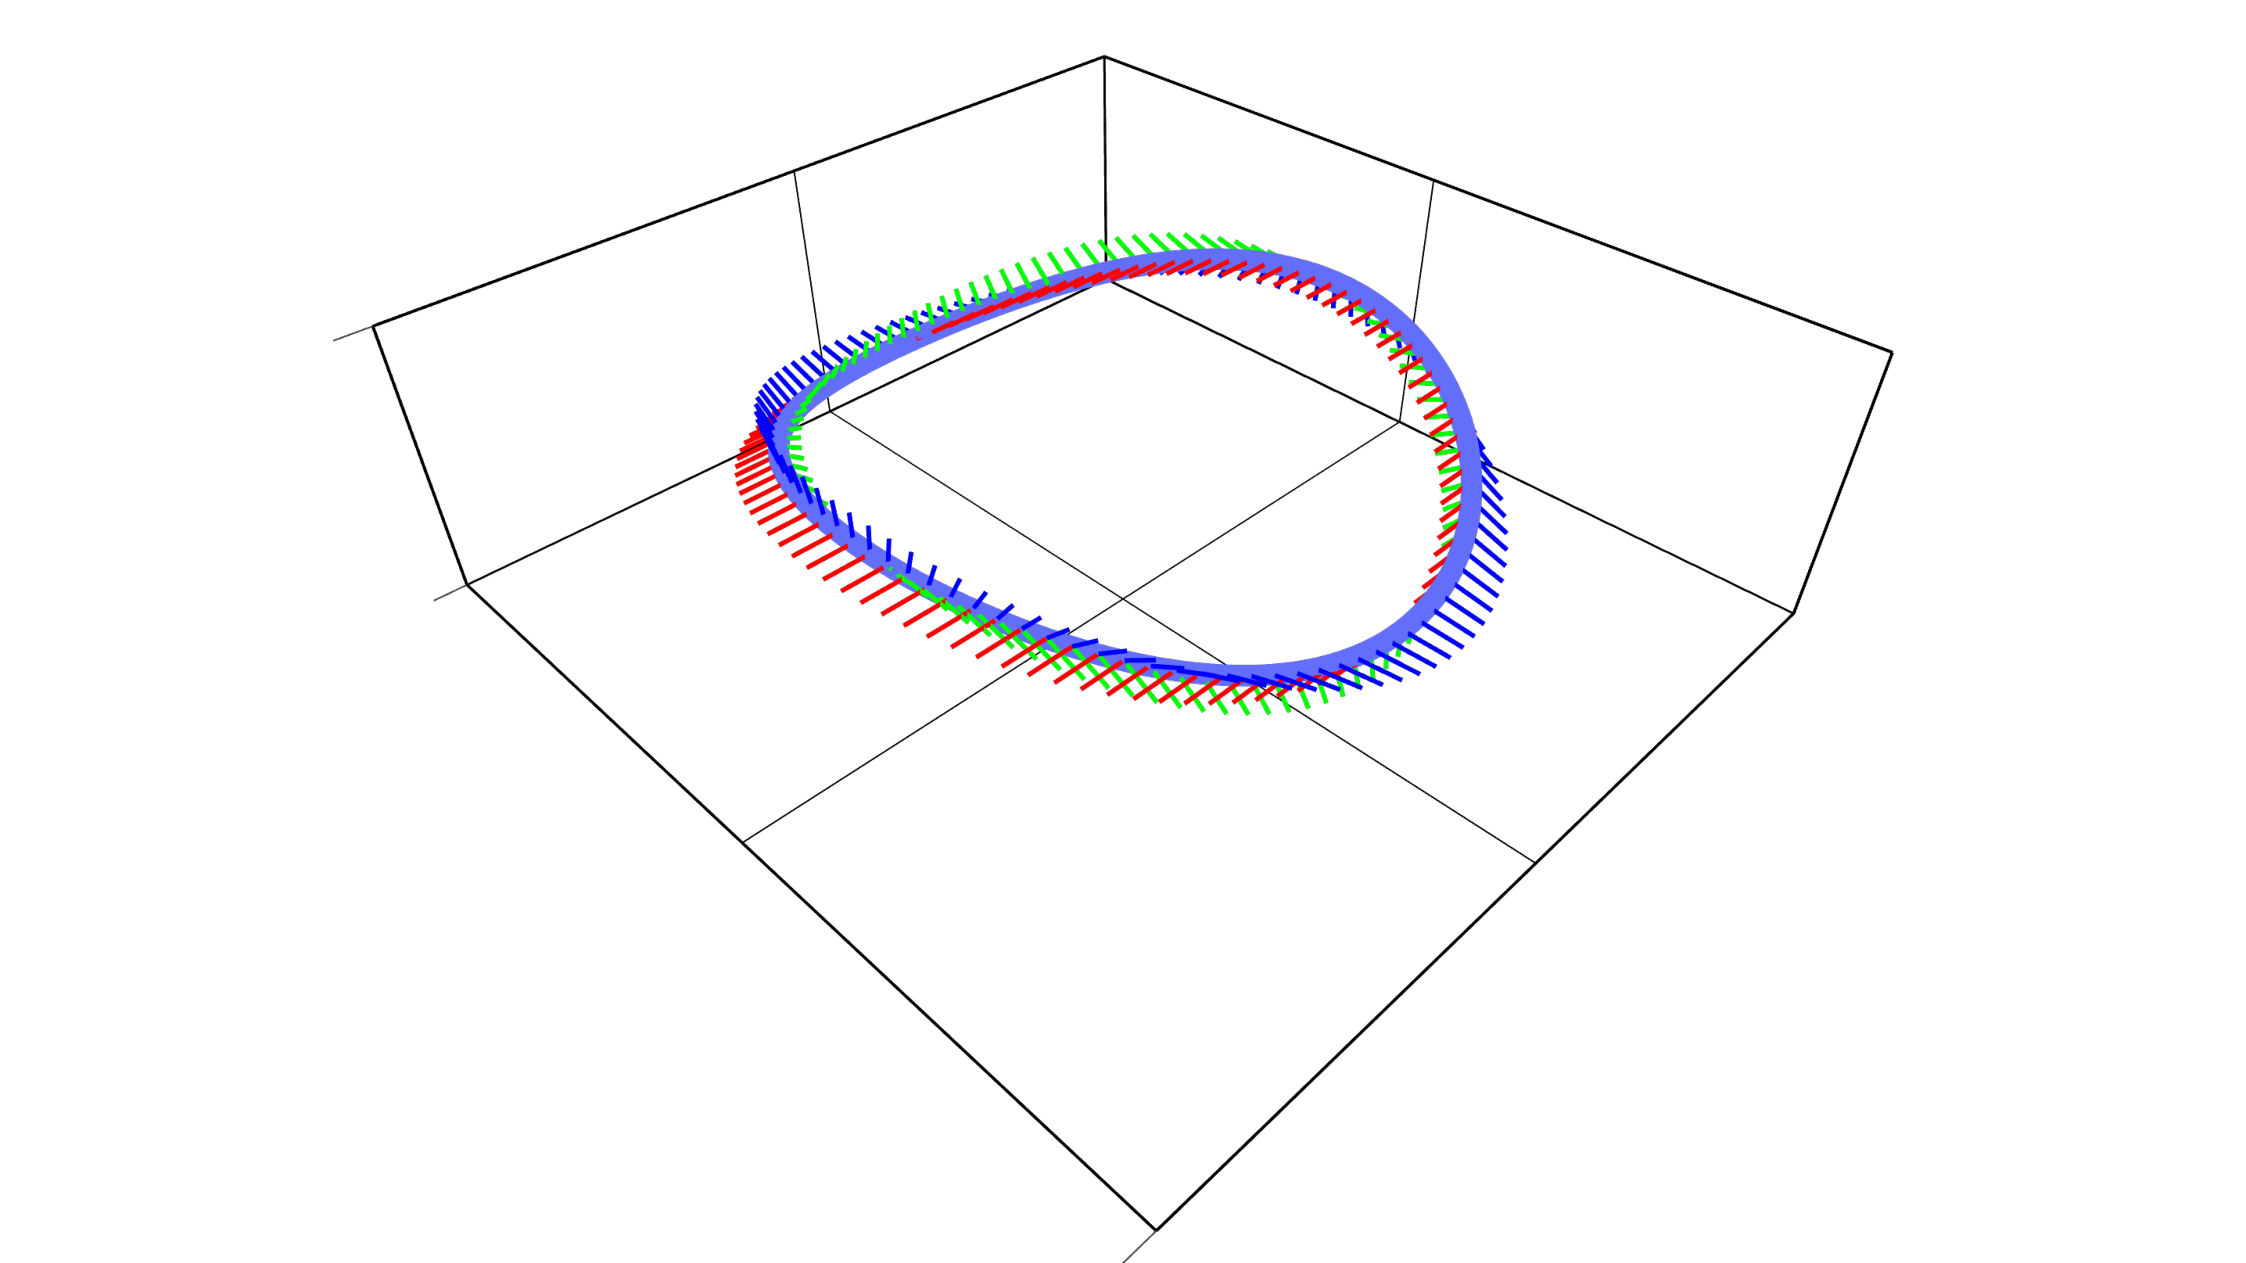
\includegraphics[width=.8\linewidth]{figures/curve_with_frames.pdf}
    \caption{Curve $\mathcal{C}$ in $\mathbb{R}^3\times\text{SO}(3)$. Orientation frames are depicted using RGB axes.}
    \label{fig:curvewithframes}
\end{figure}

The task can be achieved determining a control input $\boldsymbol{\xi}$ such that the body follows the curve $\mathcal{C}$ under a kinematic model. Although the system model was developed using the tuple representation of $\mathbb{R}^3\times\text{SO}(3)$, in this section we adopt the independent representation of $\text{ISE}(3)$, as it simplifies the control design. Note that this identification is always possible, since for any $\mathbf{H}\in\text{ISE}(3)$, we can identify $\boldsymbol{\chi}=(\mathbf{p}, \mathbf{R})$ using the following map
\begin{align}
    \begin{split}
        \mathbf{H} &\mapsto (\mathbf{B}\mathbf{H}\mathbf{c},\, \mathbf{A}\mathbf{H}\mathbf{A}^\top) \in \mathbb{R}^3\times\text{SO}(3)\\
        \mathbf{A} &= \begin{bmatrix}
            \mathbf{I}_{3\times 3} & \mathbf{0}_{3\times 4}
        \end{bmatrix}, \quad
        \mathbf{B} = \begin{bmatrix}
            \mathbf{0}_{3\times 3} & \mathbf{I}_{3\times 3} & \mathbf{0}
        \end{bmatrix}, \quad
        \mathbf{c} = \begin{bmatrix}
            \mathbf{0}^\top & 1
        \end{bmatrix}^\top.
    \end{split}
\end{align}

Now, let the system state be represented by an element $\mathbf{H}(t)\in\text{ISE}(3)$, with a generalized twist $\boldsymbol{\xi}\in\mathbb{R}^6$. Given a curve parametrization $\mathbf{H}_d(s)\in\text{ISE}(3)$, we want to compute a vector field $\Psi:\text{ISE}(3)\to\mathbb{R}^6$ such that if $\boldsymbol{\xi} = \Psi(\mathbf{H})$, the system follows the curve $\mathcal{C}$. The system can be described through the following single integrator model:
\begin{align}
% \begin{split}
    \dot{\mathbf{H}} &= \SL[\boldsymbol{\xi}]\mathbf{H}\label{eq:first-order-system-cba}
% \end{split} 
\end{align}

In order to use our vector field methodology, we define an EE-distance function $\widehat{D}: \text{ISE}(3) \times \text{ISE}(3) \to \mathbb{R}_+$ between two elements $\mathbf{V}, \mathbf{W}$ in the group $\text{ISE}(3)$ as follows
\begin{align}
    \widehat{D}(\mathbf{V}, \mathbf{W}) = \| \log(\mathbf{V}^{-1}\mathbf{W}) \|_F. \label{eq:cba-distance-new}
\end{align}
Note that this is exactly the same distance as defined in \cref{ch:kinematic}, and so it possesses the same properties.
\begin{remark}
    In our original approach, we treat our system directly in $\mathbb{R}^3\times\text{SO}(3)$, and use the following distance function between two tuples:
    \begin{align}
        \widehat{D}(\mathbf{p}_1, \mathbf{R}_1, \mathbf{p}_2, \mathbf{R}_2) \equiv \frac{1}{2}\left(\|\mathbf{p}_1 - \mathbf{p}_2\|^2 + \beta\left\|\mathbf{I} - \mathbf{R}_2^{T}\mathbf{R}_1\right\|^2_F\right). \label{eq:cba-distance}
    \end{align}
    Although they are not equivalent, the change in the distance function will maintain consistency with our generalization to matrix Lie groups.
    
    Note that the distance in \eqref{eq:cba-distance} is left-invariant, and although it lacks a chainability proof, we can still show that the vector field it renders has a measure zero set of singularities. This change of distance is beneficial, as it aligns with all the properties and proofs given.
\end{remark}

We will assume that the target curve $\mathcal{C}$ is twice differentiable, closed, and without self-intersections. Thus, for an element $\mathbf{H}\in\text{ISE}(3)$ and a curve parametrization $\mathbf{H}_d(s)\in\text{ISE}(3)$, the vector field has the same expression
\begin{align}
    \Psi(\mathbf{H}) = k_N(\mathbf{H})\boldsymbol{\xi}_N(\mathbf{H}) + k_T(\mathbf{H})\boldsymbol{\xi}_T(\mathbf{H}).
\end{align}
By following this vector field, the system \eqref{eq:first-order-system-cba} will converge to and follow the target curve.

\subsection{Computation of the EE-distance}\label{sec:collaborative-ee-distance-computation}
It is possible to use an simple algorithm to compute the defined EE-distance \eqref{eq:cba-distance-new}. First, note that for any elements $\mathbf{V}, \mathbf{W}\in\text{ISE}(3)$, we can write
\begin{align}
    \mathbf{V}^{-1}\mathbf{W} = \mathbf{Z} = \begin{bmatrix}
        \mathbf{R}_v^\top\mathbf{R}_w & \mathbf{0} & \mathbf{0}\\
        \mathbf{0} & \mathbf{I} & \mathbf{p}_w - \mathbf{p}_v\\
        \mathbf{0} & \mathbf{0} & 1
    \end{bmatrix} = \begin{bmatrix}
        \mathbf{Q} & \mathbf{0} & \mathbf{0}\\
        \mathbf{0} & \mathbf{I} & \mathbf{u}\\
        \mathbf{0} & \mathbf{0} & 1
    \end{bmatrix},
\end{align}
where $\mathbf{R}_v$, $\mathbf{R}_w$, $\mathbf{p}_v$, and $\mathbf{p}_w$ are the rotation matrices and positions of $\mathbf{V}$ and $\mathbf{W}$, respectively. Using \vthree{Cayley-Hamilton's theorem and properties of block triangular matrices, it is possible to write}
\begin{align}
    \log(\mathbf{Z}) &= \begin{bmatrix}
        \log\mathbf{Q} & \mathbf{0} & \mathbf{0}\\
        \mathbf{0} & \mathbf{0} & \mathbf{u}\\
        \mathbf{0} & \mathbf{0} & 0
    \end{bmatrix}.
\end{align}
Now, applying the Frobenius norm, we have
\begin{align}
    \|\log(\mathbf{Z})\|_F^2 &= \tr\bigl(\log(\mathbf{Z})^\top\log(\mathbf{Z})\bigr)^\frac{1}{2} = \tr\!\left(\begin{bmatrix}
        (\log\mathbf{Q})^\top\log\mathbf{Q} & \mathbf{0} & \mathbf{0}\\
        \mathbf{0} & \mathbf{0} & 0\\
        \mathbf{0} & \mathbf{0} & \mathbf{u}^\top\mathbf{u}
    \end{bmatrix}\right)^\frac{1}{2} \\
    &= \sqrt{\|\log\mathbf{Q}\|_F^2 + \|\mathbf{u}\|^2} = \sqrt{2\theta^2 + \|\mathbf{u}\|^2},
\end{align}
where $\theta$ is the rotation angle as in \cref{app:rodrigues-formula}. Thus, in this case the algorithm to compute the EE-distance is a simplified version of \cref{alg:dhat-se3}:
\begin{algorithm}
    \caption{Computation of $\widehat{D}(\mathbf{V}, \mathbf{W})$ in $\text{ISE}(3)$}
    \begin{algorithmic}[1]\label{alg:dhat-ise3}
        \Statex \textbf{Input:} Matrices $\mathbf{V}, \mathbf{W}$
        \Statex \textbf{Output:} Distance $\widehat{D}$
        % \Statex
        
        \State Compute $\mathbf{Z} \gets \mathbf{V}^{-1}\mathbf{W}$
        \State Extract $\mathbf{Q} \gets \text{rotation part of } \mathbf{Z}$ and $\mathbf{u} \gets \text{translation part of } \mathbf{Z}$

        \State $u \gets \frac{1}{2} (\tr(\mathbf{Q}) - 1)$
        \State $v \gets \frac{1}{2\sqrt{2}} \|\mathbf{Q} - \mathbf{Q}^\top\|_F$
        \State $\theta \gets \text{atan2}(v, u)$
        \State $\widehat{D} \gets \sqrt{2\theta^2 + \mathbf{u}^\top\mathbf{u}}$
    \end{algorithmic}
\end{algorithm}

% To begin, we define an error function $\widehat{D}\equiv\widehat{D}(\mathbf{p}, \mathbf{R}, \mathbf{p}_d, \mathbf{R}_d)$ that measures the discrepancy between a pose $(\mathbf{p}, \mathbf{R})$ and a desired pose $(\mathbf{p}_d, \mathbf{R}_d)$. The error function is expressed as follows
% \begin{equation}
%     \widehat{D}(\mathbf{p}, \mathbf{R}, \mathbf{p}_d, \mathbf{R}_d) \equiv \frac{1}{2}\left(\|\mathbf{p} - \mathbf{p}_d\|^2 + \beta\left\|\mathbf{I} - \mathbf{R}_d^{T}\mathbf{R}\right\|^2_F\right),\! \label{eq:errorfuncDtilde}
% \end{equation}
% where $\beta$ is a scaling parameter in squared meters utilized to maintain dimensional consistency. The Frobenius norm measures the parallelism of the rotation matrices columns, allowing parameter $\beta$ to balance position and orientation errors.

\section{Adaptive control}
The problem addressed in this section focuses on designing an adaptive controller to guide a manipulated object along a predefined curve $\mathcal{C} \subset \mathbb{R}^3\times \text{SO}(3)$, despite uncertainties in the inertial and geometric parameters. With $N$ agents involved in the manipulation process, a decentralized control law is devised for each agent, assuming they can measure the pose and velocity of the object's measurement point but lack precise knowledge of their positions relative to it. The goal is to provide the necessary total wrench $\boldsymbol{\tau}$ to ensure the system's velocity converges to the vector field $\Psi$, thereby enabling the object to follow the curve $\mathcal{C}$.

In this section, we modify the adaptive control strategy proposed by \cite{Culbertson2021}. In their approach, an error vector is established between the system velocity and a velocity reference, resulting in a non-autonomous system. In contrast, our method defines the velocity error $\boldsymbol{\zeta}$ with respect to the vector field, thereby establishing an autonomous system. This error vector is expressed as:
\begin{equation}
    \boldsymbol{\zeta} = \dot{\boldsymbol{\chi}} - \Psi,\label{eq:errorvector-s}
\end{equation}
If the dynamic controller guarantees that $\boldsymbol{\zeta}=0$, the system follows the integrator model \eqref{eq:first-order-system-cba}, with the vector field $\Psi$ acting as its input. Therefore, as shown in \cref{ch:vector_field}, we anticipate that the system will exhibit the desired behavior. To develop the adaptive control strategy, we first define our reference model.

Given that the system is overactuated (meaning multiple sets of control inputs $\boldsymbol{\tau}_i$ produce identical object dynamics), each agent can contribute a portion of the control effort. Thus, we define a set of $N$ positive constants $\alpha_i$, ensuring $\sum_{i=1}^N\alpha_i=1$. Furthermore, analogously to the Euler-Lagrange formulation, the reference model can be linearly parametrized. Thus, the reference model can be expressed as 
\begin{equation}
    \alpha _i \left(\mathbf {M}(\boldsymbol{\chi})\dot{\Psi} + \mathbf {C}(\boldsymbol{\chi},\dot{\boldsymbol{\chi}})\Psi + \mathbf {g} \right) = \mathbf{Y}_o(\boldsymbol{\chi}, \dot{\boldsymbol{\chi}}, \Psi, \dot{\Psi})\mathbf{o}_i, \label{eq:ref-model-linear-parametrization},
\end{equation}
% Furthermore, exploiting the linearity in the parameters within the equations of motion \citep{spong2020robot}, we can represent the object's dynamics using a regressor matrix $\mathbf{Y}_o$ and a parameter vector $\mathbf{o}_i$. Here, $\mathbf{o}_i = \alpha_i\mathbf{o}$ denotes a vector of the object's physical parameters, $\mathbf{o}$, such as mass or moments of inertia, scaled by $\alpha_i$:
% Analogously to the Euler-Lagrange formulation, the reference model can be linearly parametrized as
% \begin{align}
%     \boldsymbol{\tau}_i &= \mathbf{Y}_o(\boldsymbol{\chi}, \dot{\boldsymbol{\chi}}, \boldsymbol{\Psi}, \dot{\boldsymbol{\Psi}})\mathbf{o}_i, \label{eq:ref-model-linear-parametrization}
% \end{align}
where $\mathbf{Y}_o$ is the regressor matrix given by
\begin{align}
    \mathbf{Y}_o &= \begin{bmatrix}
        \ddot{\mathbf{p}}_d & -\SL[\dot{\boldsymbol{\omega}}_d]\mathbf{R}-\SL[\boldsymbol{\omega}]\SL[\boldsymbol{\omega}_d]\mathbf{R} & \mathbf{0}\\
        \mathbf{0} & \SL[\ddot{\mathbf{p}}_d]\mathbf{R} + \SL[\boldsymbol{\omega}]\SL[\dot{\mathbf{p}}_d]\mathbf{R} - \SL[\boldsymbol{\omega}_d]\SL[\dot{\mathbf{p}}]\mathbf{R} & \mathbf{R}\mathcal{J}\bigl(\mathbf{R}\dot{\boldsymbol{\omega}}_d\bigr) + \SL[\boldsymbol{\omega}]\mathbf{R}\mathcal{J}\bigl(\mathbf{R}^\top\boldsymbol{\omega}_d\bigr)
    \end{bmatrix},
\end{align}
where $\mathcal{J}:\mathbb{R}^3\to\mathbb{R}^{3\times6}$ is the following map
\begin{align}
    \mathcal{J}\bigl([a_1\ a_2\ a_3]^\top\bigr)=\begin{bmatrix}
        a_1 & a_2 & a_3 & 0 & 0 & 0 \\
        0 & a_1 & 0 & a_2 & a_3 & 0 \\
        0 & 0 & a_1 & 0 & a_2 & a_3
    \end{bmatrix}.
\end{align}
The term $\mathbf{o}_i$ is the parameter vector given by
\begin{align}   
    \mathbf{o}_i &= \alpha_i\begin{bmatrix}
        m & m\mathbf{r}_p & \mathbb{I}_{p11} & \mathbb{I}_{p12} & \mathbb{I}_{p22} & \mathbb{I}_{p23} & \mathbb{I}_{p33}
    \end{bmatrix}^\top,
\end{align}
where $\mathbb{I}_{pij}$ are the elements of the inertia matrix $\mathbb{I}_p^\mathfrak{B}$ at the $i^{th}$ row and $j^{th}$ column. Note that, given that the inertia tensor is symmetric, we only need to consider the upper triangular part of the matrix. Also, note that the sum $\sum_{i=1}^N\mathbf{Y}_o\mathbf{o}_i=\mathbf{Y}_o\mathbf{o}$ results in the total wrench $\boldsymbol{\tau}$ applied to the object. Moreover, since the agents estimate the scaled vector $\mathbf{o}_i$, the constants $\alpha_i$ need not be known a priori.

Next, we propose the following control law
\begin{equation}
    \boldsymbol{\tau}_i = \mathbf{G}(\boldsymbol{\chi}, \hat{\mathbf{r}}_i)^{-1}\boldsymbol{\eta}_i,\label{eq:controlLawTaui}
\end{equation}
where $\hat{\mathbf{r}}_i$ represents the estimate of $i^{th}$ agent's displacement with respect to the measurement point, and
\begin{equation}
    \boldsymbol{\eta}_i = \mathbf{Y}_o\hat{\mathbf{o}}_i - \mathbf{K}_D\boldsymbol{\zeta}, \label{eq:controlLawEtai}
\end{equation}
where $\mathbf{K}_D$ is a positive definite matrix, and $\hat{\mathbf{o}}_i$ is the $i^{th}$ agent's estimate of the object's parameters. 

% It is essential to note that:
% \begin{equation}
%     \mathbf{G}_i\mathbf{G}(\hat{\mathbf{r}}_i)^{-1} = \mathbf{I} - \mathbf{G}(\widetilde{\mathbf{r}}_i), \label{eq:relationGiGiInvtoProof}
% \end{equation}
% where $\widetilde{\mathbf{r}}_i = \hat{\mathbf{r}}_i - \mathbf{r}_i$.

If we let $\widetilde{\mathbf{r}}_i = \hat{\mathbf{r}}_i - \mathbf{r}_i$, we can achieve the following linear parametrization:
\begin{equation}
    -\mathbf{G}(\boldsymbol{\chi}, \widetilde{\mathbf{r}}_i)\boldsymbol{\eta}_i = \mathbf{Y}_r\left(\boldsymbol{\eta}_i, \boldsymbol{\chi}\right)\widetilde{\mathbf{r}}_i. \label{eq:linearParametrizationYrforEta}
\end{equation}
With this parametrization and the other expressions, we propose the following adaptation laws:
\begin{align}
    \dot{\hat{\mathbf{o}}}_i &= -\boldsymbol{\Gamma}_o\mathbf{Y}^\top_o\left(\boldsymbol{\chi},\dot{\boldsymbol{\chi}},\Psi, \dot{\Psi}\right)\boldsymbol{\zeta},  \label{eq:adaptiveOhat}\\
    \dot{\hat{\mathbf{r}}}_i &= -\boldsymbol{\Gamma}_r\mathbf{Y}^\top_r\left(\boldsymbol{\eta}_i, \boldsymbol{\chi}\right)\boldsymbol{\zeta},  \label{eq:adaptiveRhat}
\end{align}
where $\boldsymbol{\Gamma}_o$ and $\boldsymbol{\Gamma}_r$ are definite positive matrices corresponding to the adaptation gains. With the proposed control law \eqref{eq:controlLawTaui} and adaptation laws \eqref{eq:adaptiveOhat} and \eqref{eq:adaptiveRhat}, we can guarantee that the system follows the curve $\mathcal{C}$ as proven in the following theorem.
\begin{theorem}
    Under the adaptive control laws \eqref{eq:controlLawTaui} and \eqref{eq:controlLawEtai}, and adaptation laws \eqref{eq:adaptiveOhat} and \eqref{eq:adaptiveRhat}, the system converges to and follows the curve $\mathcal{C}$.
\end{theorem}
\begin{proof}
    Consider the following Lyapunov function candidate
    \begin{equation}
        V = \frac{1}{2}\left( \boldsymbol{\zeta}^\top \mathbf {M} \boldsymbol{\zeta} + \sum _{i=1}^{N} \widetilde{\mathbf{o}}_i^\top \boldsymbol{\Gamma }_o^{-1}\widetilde{\mathbf{o}}_i + \widetilde{\mathbf{r}}_i^\top \boldsymbol{\Gamma }_r^{-1} \widetilde{\mathbf{r}}_i \right),
    \end{equation}
    where $\widetilde{\mathbf {o}}_i = \hat{\mathbf{o}}_i - \mathbf{o}_i$ represents the parameter estimation error for the $i^{th}$ agent.

    Since the true parameters do not vary in time, i.e. $\dot{\widetilde{\mathbf {o}}}_i = \dot{\hat{\mathbf{o}}}_i$ and $\dot{\widetilde{\mathbf {r}}}_i = \dot{\hat{\mathbf{r}}}_i$, the time derivative of the Lyapunov candidate yields
    \begin{equation}
        \dot{V} = \boldsymbol{\zeta}^\top \mathbf{M} \dot{\boldsymbol{\zeta}} + \frac{1}{2} \boldsymbol{\zeta}^\top \dot{\mathbf{M}} \boldsymbol{\zeta} + \sum\limits_{i=1}^{N} \widetilde{\mathbf{o}}_i^\top \boldsymbol{\Gamma}_o^{-1} \dot{\hat{\mathbf{o}}}_i + \widetilde{\mathbf{r}}_i^\top \boldsymbol{\Gamma}_r^{-1}\dot{\hat{\mathbf{r}}}_i.
        \label{eq:adaptive-lyapunov-derivative}
    \end{equation}
    Using the fact that $\dot{\boldsymbol{\zeta}} = \ddot{\boldsymbol{\chi}} - \dot{\Psi}$ and $\dot{\boldsymbol{\chi}} = \boldsymbol{\zeta} + \Psi$, along with the system dynamics equation \eqref{eq:tau} and relation \eqref{eq:tauNtauIrelation}, and \eqref{eq:ref-model-linear-parametrization}, we can express the first term as
    \begin{align} 
    \begin{split}
        \boldsymbol{\zeta}^\top \mathbf {M} \dot{\boldsymbol{\zeta}} &= \boldsymbol{\zeta}^\top\mathbf{M}\bigl(\ddot{\boldsymbol{\chi}} - \dot{\Psi}\bigr)
        = \boldsymbol{\zeta}^\top\bigl(\boldsymbol{\tau} - \mathbf{C}\dot{\boldsymbol{\chi}} - \mathbf{g} - \mathbf{M}\dot{\Psi}\bigr)\\
        &= \boldsymbol{\zeta}^\top\Biggl(\biggl(\sum_{i=1}^N\mathbf{G}(\boldsymbol{\chi}, \mathbf{r}_i)\boldsymbol{\tau}_i\biggr) -\mathbf{C}\Psi - \mathbf{C}\boldsymbol{\zeta} - \mathbf{g} - \biggl(-\mathbf{C}\Psi-\mathbf{g}+\sum_{i=1}^N\mathbf{Y}_o\mathbf{o}_i\biggr)\Biggr)\\
        &= \boldsymbol{\zeta}^\top\Biggl( - \mathbf{C}\boldsymbol{\zeta}+\sum_{i=1}^N\mathbf{G}(\boldsymbol{\chi}, \mathbf{r}_i)\boldsymbol{\tau}_i - \mathbf{Y}_o\mathbf{o}_i \Biggr).
    \end{split} \label{eq:partial-term-of-adaptive1}
    \end{align} 
    Now, using equations \eqref{eq:controlLawTaui}, \eqref{eq:controlLawEtai} and \eqref{eq:linearParametrizationYrforEta}, the first term in \eqref{eq:partial-term-of-adaptive1} can be rewritten as
    \begin{align}
        \boldsymbol{\zeta}^\top \mathbf {M} \dot{\boldsymbol{\zeta}} &= \boldsymbol{\zeta}^\top\Biggl( - \mathbf{C}\boldsymbol{\zeta} + \sum_{i=1}^N\mathbf{G}(\boldsymbol{\chi}, \mathbf{r}_i)\mathbf{G}(\boldsymbol{\chi}, \hat{\mathbf{r}}_i)^{-1}\boldsymbol{\eta}_i - \mathbf{Y}_o\mathbf{o}_i\Biggr)\\
        &= \boldsymbol{\zeta}^\top\Biggl(- \mathbf{C}\boldsymbol{\zeta}+\sum_{i=1}^N(\mathbf{I}-\mathbf{G}(\boldsymbol{\chi}, \widetilde{\mathbf{r}}_i))\boldsymbol{\eta}_i - \mathbf{Y}_o\mathbf{o}_i \Biggr)\\
        &= \boldsymbol{\zeta}^\top\Biggl(- \mathbf{C}\boldsymbol{\zeta} + \sum_{i=1}^N \mathbf{Y}_o\hat{\mathbf{o}}_i + \mathbf{Y}_r\widetilde{\mathbf{r}}_i - \mathbf{Y}_o\mathbf{o}_i- \mathbf{K}_D\boldsymbol{\zeta} \Biggr)\\
        &= \boldsymbol{\zeta}^\top\Biggl(- \mathbf{C}\boldsymbol{\zeta} + \sum_{i=1}^N \mathbf{Y}_o\widetilde{\mathbf{o}}_i + \mathbf{Y}_r\widetilde{\mathbf{r}}_i - \mathbf{K}_D\boldsymbol{\zeta} \Biggr). \label{eq:partial-term-of-adaptive2}
    \end{align}

    Finally, substituting \eqref{eq:partial-term-of-adaptive2} into \eqref{eq:adaptive-lyapunov-derivative} renders the following result
    \begin{align}
    % \begin{split}
        \dot{V} &= \frac{1}{2}\boldsymbol{\zeta}^\top \bigl(\dot{\mathbf{M}}- 2\mathbf{C}\bigr) \boldsymbol{\zeta} + \sum\limits_{i=1}^{N} \widetilde{\mathbf{o}}_i^\top \boldsymbol{\Gamma}_o^{-1} \dot{\hat{\mathbf{o}}}_i + \widetilde{\mathbf{r}}_i^\top \boldsymbol{\Gamma}_r^{-1}\dot{\hat{\mathbf{r}}}_i + \boldsymbol{\zeta}^\top\bigl(\mathbf{Y}_o\widetilde{\mathbf{o}}_i + \mathbf{Y}_r\widetilde{\mathbf{r}}_i - \mathbf{K}_D\boldsymbol{\zeta} \bigr).
        % \end{split}
    \end{align}
    Substituting adaptation laws \eqref{eq:adaptiveOhat} and \eqref{eq:adaptiveRhat}, and using the fact that $\dot{\mathbf{M}} - 2\mathbf{C}$ is skew-symmetric, we have
    \begin{align}
        \dot{V} &= \sum\limits_{i=1}^{N} \widetilde{\mathbf{o}}_i^\top \mathbf{Y}^\top_o\boldsymbol{\zeta}  - \widetilde{\mathbf{r}}_i^\top\mathbf{Y}^\top_r\boldsymbol{\zeta} + \boldsymbol{\zeta}^\top\mathbf{Y}_o\widetilde{\mathbf{o}}_i + \boldsymbol{\zeta}^\top\mathbf{Y}_r\widetilde{\mathbf{r}}_i - \boldsymbol{\zeta}^\top\mathbf{K}_D\boldsymbol{\zeta}.
    \end{align}
    Since all terms are scalars, we can transpose the first two terms and achieve the following result
    \begin{align}
        \dot{V} = \sum\limits_{i=1}^{N}\boldsymbol{\zeta}^\top\mathbf{K}_D\boldsymbol{\zeta} = -N\boldsymbol{\zeta}^\top\mathbf{K}_D\boldsymbol{\zeta} \le 0.
    \end{align}
    Since $N$ is positive and $\mathbf{K}_D$ is definite positive, $\boldsymbol{\zeta}$ converges to zero as $t\to\infty$. This implies that velocity error is zero and the system behaves as the kinematic model \eqref{eq:first-order-system-cba}. Thus we can invoke \cref{thm:convergence-vector-field} to conclude that the system converges to and follows the curve $\mathcal{C}$.
\end{proof}

The connection of both controllers is shown in the block diagram of \cref{fig:collaborative-full-diagram}.
\begin{figure}[ht]
    \centering
    \resizebox{\textwidth}{!}{%
    \begin{tikzpicture}[
        block/.style={draw, rectangle, minimum height=1.2cm, minimum width=2.4cm, align=center},
        arrow/.style={->, >=stealth, thick},
        label/.style={font=\small},
        sumblock/.style={draw, circle, minimum size=0.8cm}
    ]
    
    % Nodes
    \node[block] (kinematic) {Vector Field};
    \node[block, right=2cm of kinematic] (refmodel) {Reference\\Model};
    % \node[block, right=2cm of kinematic] (plant) {Plant \\ $P(\theta)\to P_c(\theta_c)$};
    \node[block, right=1cm of refmodel] (control) {Dynamic\\Controller};
    \node[block, above=0.75cm of control] (estimation) {Estimation\\of $\mathbf{o}_i, \mathbf{r}_i$};
    \node[block, above=1cm of estimation, xshift=-1cm] (mapping) {Mapping\\$\mathbb{R}^3\times\text{SO}(3)\to\text{ISE}(3)$};
    \node[block, right=1cm of control] (plant) {System};
    \node[left=0.75cm of kinematic,yshift=-0.25cm] (input) {Curve $\mathcal{C}$};
    \node[sumblock, left=2cm of estimation, yshift=-0.25cm] (sum) {};
    \node at ([xshift=0.2cm]sum.west) {\(+\)};
    \node at ([yshift=-0.2cm]sum.north) {\(-\)};
    \node[right=1.5cm of plant] (output) {$\boldsymbol{\chi}$};
    
    % Arrows between blocks
    \draw[arrow] (input) -- ($(kinematic.west)+(0,-0.25cm)$);
    \draw[arrow] (plant.east) -- (output);
    % Ends in refmodel
    \draw[arrow] (kinematic) -- node[below, label] {$\Psi, \dot{\Psi}$} (refmodel);
    \draw[arrow] ($(plant.east)+(0.75, 0)$) |- ($(refmodel.south)+(0,-1)$) -| node[right, label,yshift=0.25cm] {$\boldsymbol{\chi}, \dot{\boldsymbol{\chi}}$} (refmodel.south);
    % Ends in System
    \draw[arrow] (control) -- node[above, label] {$\boldsymbol{\tau}_i$} (plant);
    % Ends in mapping
    \draw[arrow] ($(plant.east)+(0.75,0)$) |- (mapping.east) node[right, yshift=0.25cm, label] {$\boldsymbol{\chi}\in\mathbb{R}^3\times\text{SO}(3)$};
    % Ends in Estimation
    \draw[arrow] (sum.east) -- node[below,label] {$\boldsymbol{\zeta}$} ($(estimation.west)+(0,-0.25)$);
    \draw[arrow] ($(plant.east)+(0.75,0)$) |- (estimation.east) node[right, label, yshift=0.25cm] {$\boldsymbol{\chi}, \dot{\boldsymbol{\chi}}$};
    \draw[arrow] ($(refmodel.east)+(0.5,0)$) |- ($(estimation.west)+(0,0.25)$);
    % Ends in Vector Field
    \draw[arrow] (mapping.west) node[left, yshift=0.25cm, label] {$\mathbf{H}\in\text{ISE}(3)$} -| ($(kinematic.west)+(-0.75,1)$) |- ($(kinematic.west)+(0,0.25)$);
    % Ends in Control
    \draw[arrow] (estimation.south) -- node[right, label] {$\widehat{\mathbf{o}}_i, \widehat{\mathbf{r}}_i$} (control.north);
    \draw[arrow] (refmodel.east) -- node[below, label] {$\mathbf{Y}_o$} (control.west);
    \draw[arrow] ($(estimation.west)+(-0.25,-0.25)$) |- ($(control.west)+(0,0.25)$);
    \draw[arrow] ($(plant.east)+(0.75, 0)$) |- ($(control.south)+(0,-0.5)$) -| node[right, label,yshift=0.25cm] {$\boldsymbol{\chi}$} (control.south);
    % Ends in summation block
    \draw[arrow] ($(kinematic.east)+(1,0)$) |- node[left, label] {$\Psi$} (sum.west);
    \draw[arrow] ($(plant.east)+(0.75,0)$) |- ($(sum.north)+(0,1)$) -| node[left, label] {$\dot{\boldsymbol{\chi}}$} (sum.north);
    \end{tikzpicture}%
    }
    \caption{Block diagram of the collaborative manipulation control framework.}
    \label{fig:collaborative-full-diagram}
\end{figure}
% !TeX root = main.tex
\chapter{Results and Discussion}
\section{Kinematic control}
\subsection{The target curve}
The considered curve $\mathcal{C}$ was based on the hyperbolic paraboloid while rotating in the $x$ axis in the world frame. Its parametrization is expressed as 
\begin{align}
    \mathbf{H}_d(s) = \begin{bmatrix}
        1 & \ \ 0 & 0 & rc_\theta\\
        0 & \ \ c_\theta & s_\theta & rs_\theta\\
        0 & -s_\theta & c_\theta & b + dr^2(c_\theta^2 - s_\theta^2)\\
        0 & \ \ 0 & 0 & 1
    \end{bmatrix},
\end{align}
where $c_\theta$ and $s_\theta$ denotes $\cos\theta$ and $\sin\theta$ respectively, $\theta = 2\pi s$, $b=\qty{1}{\meter}$, $d=\qty{0.2}{\meter}$, and $r=\qty{1}{\meter}$.

\subsection{The choice of S map}
Let $\boldsymbol{\xi} = [\xi_1 \ \xi_2 \ \xi_3 \ \xi_4 \ \xi_5 \ \xi_6]^\top$. The map $\SL$ used is:
\begin{equation}
    \SL[\boldsymbol{\xi}] = \left[\begin{array}{cccc} 
    \ 0 & -\xi_6 & \ \ \xi_5 & \ \ \xi_1 \\
    \ \ \xi_6 & \ 0 & -\xi_4 & \ \ \xi_2 \\
    -\xi_5 & \ \ \xi_4 & \ 0 & \ \ \xi_3 \\
    \ 0 & \ 0 & \ 0 & \ 0
    \end{array}\right].
\end{equation}
The basis $\mathbf{E}_1, ... ,\mathbf{E}_6$ of the Lie algebra $\mathfrak{se}(3)$ can be obtained by $\mathbf{E}_k = \SL[\mathbf{e}_k]$, where $\mathbf{e}_k$ are the columns of the $6 \times 6$ identity matrix. Geometrically, the interpretation for this choice of basis is that $\boldsymbol{\xi}$ is the classical \emph{twist} in mechanics. More precisely, $\boldsymbol{\omega} \triangleq [\xi_4 \  \xi_5 \  \xi_6]^\top$ represents the $x$, $y$ and $z$ components of the angular  velocity  measured in the fixed frame, whereas $\mathbf{v} \triangleq [\xi_1 \  \xi_2 \  \xi_3]^\top$ represents the $x, y$ and $z$ velocities of the virtual point at the origin of the fixed frame, measured in this fixed frame. This is related to the object's linear velocity $\dot{\mathbf{p}}$  by $\dot{\mathbf{p}} = \boldsymbol{\omega} \times \mathbf{p} + \mathbf{v}$.

\subsection{Parameters}
The optimization problem in \eqref{eq:optimization-problem-distance-definition-point-curve} was solved by discretizing the curve $\mathcal{C}$ using $\num{5000}$ points and determining the optimal $s=s^*$ through a brute-force approach. This discretization was also used to compute $\frac{d}{ds}\mathbf{H}_d(s)$ using finite differences, which is necessary for implementing $\boldsymbol{\xi}_T = \SL^{-1}(\frac{d\mathbf{H}_d}{ds}(s^*)\mathbf{H}_d(s^*)^{-1})$. The chosen gains were $k_N(D) = \tanh(20D)$ and $k_T(D) = 1 - 0.5\tanh(D)$. The system was simulated for $\qty{15}{\second}$ using the approximation $\mathbf{H}(t+\Delta t)\approx \exp(\SL[\Psi]\Delta t)\mathbf{H}(t)$, with a time step of $\Delta t=\qty{0.01}{\second}$. The initial condition $\mathbf{H}(0)$was set as follows:
\begin{align}
    \mathbf{H}(0) = \begin{bmatrix}
        \frac{\sqrt{2}}{2} & -\frac{\sqrt{2}}{2} & 0 & -2\\
        \frac{\sqrt{2}}{2} & \ \frac{\sqrt{2}}{2} & 0 & -1\\
        0 & \ 0 & 1 & \ \ 0\\
        0 & \ 0 & 0 & \ 1
    \end{bmatrix}.
\end{align}

\subsection{Results}
\begin{figure}[ht!]
    \centering
    % First subfigure
    \begin{subfigure}[b]{0.32\textwidth}
        \centering
        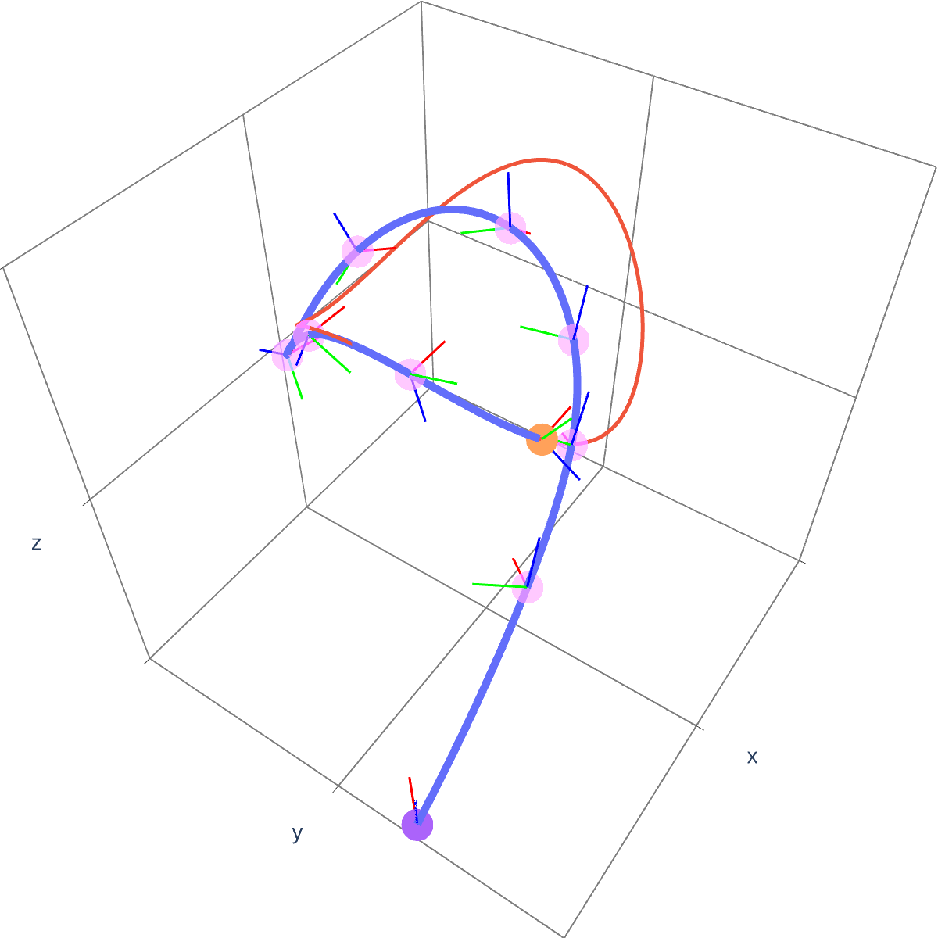
\includegraphics[width=\textwidth]{figures/vf_automatica_1.pdf} % Replace with your image
        \caption{$t\in[0, 5]s$}
        \label{fig:vfplot-first}
    \end{subfigure}
    \hfill
    % Second subfigure
    \begin{subfigure}[b]{0.32\textwidth}
        \centering
        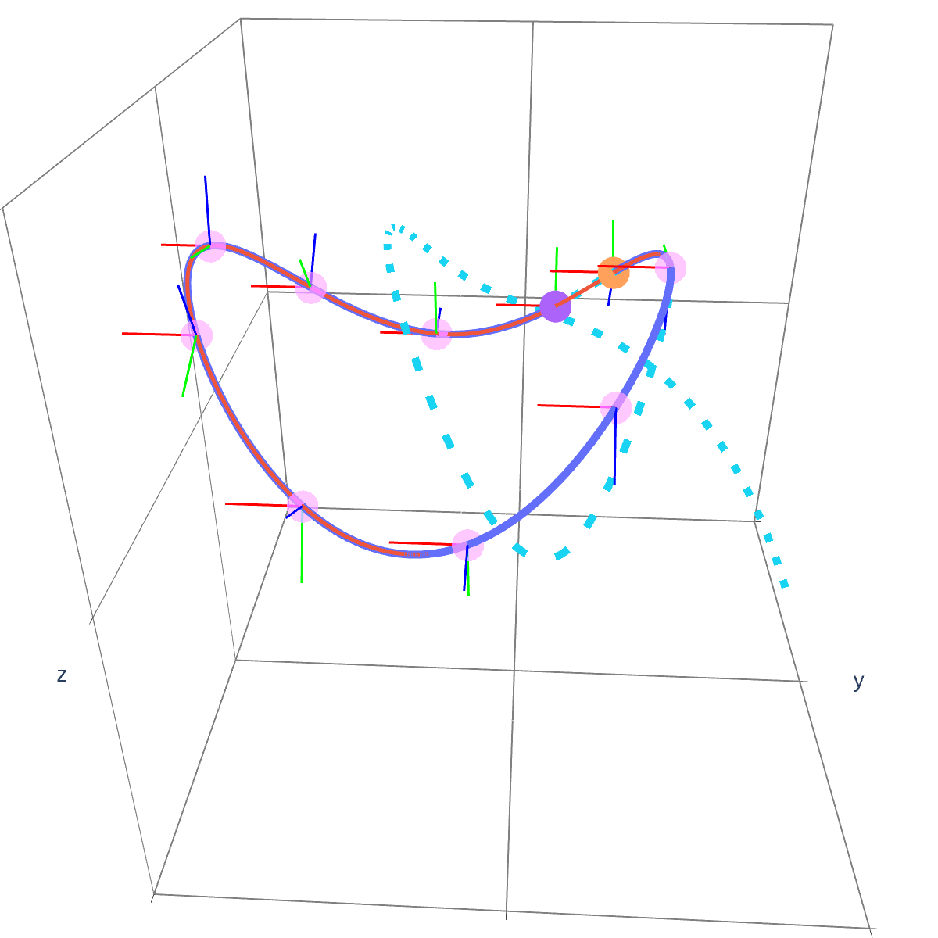
\includegraphics[width=\textwidth]{figures/vf_automatica_2.pdf} % Replace with your image
        \caption{$t\in[5, 9.7]s$}
        \label{fig:vfplot-second}
    \end{subfigure}
    \hfill
    % Third subfigure
    \begin{subfigure}[b]{0.32\textwidth}
        \centering
        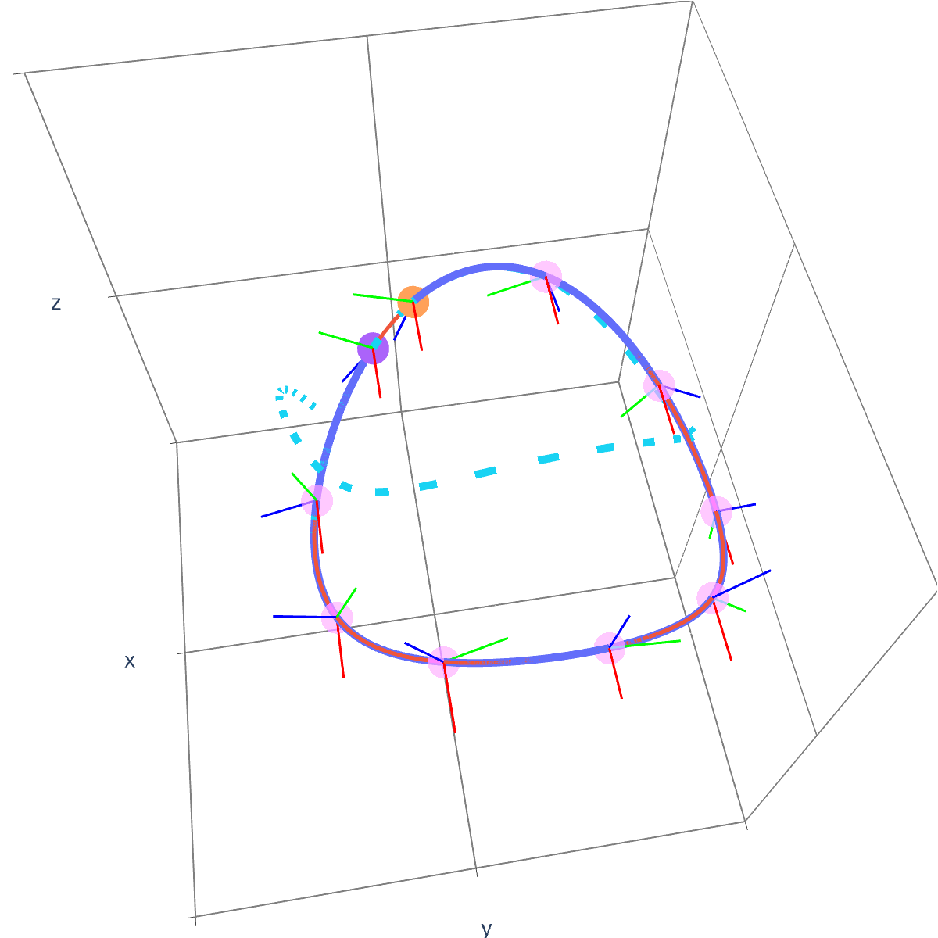
\includegraphics[width=\textwidth]{figures/vf_automatica_3.pdf} % Replace with your image
        \caption{$t\in[9.7, 14.5]s$}
        \label{fig:vfplot-third}
    \end{subfigure}
    \caption{The solid blue line depicts the system trajectory, while the solid red line indicates the target curve. The dashed light blue line represents the past trajectory. The initial and final positions are marked by purple and orange spheres, respectively. Translucent pink spheres denote intermediary positions, with orientation frames shown by RGB axes.}
    \label{fig:vfplot-trajectory}
\end{figure}
\begin{figure}[ht!]
    \centering
    \def\svgwidth{.8\linewidth}
    {\tiny\import{figures/}{distance_pos_ori_D.pdf_tex}}
    \caption{Value of EC-distance $D$, position error in centimeters and orientation error in degrees along time.}
    \label{fig:position-orientation-errors}
\end{figure}
We implemented the code in C++. On average, the computation of the vector field took $60\pm5$ milliseconds per iteration on a single core of an Intel i5-10300H @ 4.5GHz CPU, with 8 GB of RAM. On average, $99.5\%$ of this time was spent solving the optimization problem in \eqref{eq:optimization-problem-distance-definition-point-curve}. Since the optimization process is highly parallelizable -- allowing for the simultaneous computation of $\widehat{D}(\mathbf{H},\mathbf{H}_d(s))$ across different discretized $s$ -- the computational effort could be significantly reduced by leveraging parallel architectures such as GPUs, SIMD, or multi-threading. The system's trajectory is illustrated in \cref{fig:vfplot-trajectory}, while the values of the distance function $D$ are shown in \cref{fig:position-orientation-errors}. Additionally, \cref{fig:position-orientation-errors} provides a more intuitive representation of the position error (in centimeters) and the orientation error (in degrees). The results confirm that the system successfully converges to the desired curve and circulates around it as expected. Once the system reaches the curve, it remains there without deviation. Although our implementation was carried out in C++, we provide a less efficient sample code in Python for clarity and accessibility, available at \url{https://github.com/fbartelt/SE3-example/blob/main/SE3example.ipynb}.

\section{Collaborative Manipulation}
For the conduction of the adaptive control simulation of \cref{ch:collaborative}, we considered the manipulation of a large cylindrical body by six agents, aiming to converge to and circulate a curve $\mathcal{C}\in\text{ISE}(3)$. The cylindrical body had a radius $r$ of $\qty{0.25}{\meter}$, a height $h$ of $\qty{1}{\meter}$ and a mass $m$ of $\qty{1.28E3}{\kilogram}$. The measurement point $\mathbf{r}_p$ was taken as the position of the first agent $\mathbf{r}_1=[0\ 0\ 1.5]^\top$. The other agents' positions as well as the inertia tensor components are detailed in \cref{tb:parameters}.
\begin{table}[htb]
    \centering
    \begin{threeparttable}
    \caption{Adaptive simulation parameters}\label{tb:parameters}
    \begin{tabular}{clcl}
    Parameter & Value & Parameter & Value\\\hline
    $r$ & $\qty{0.25}{\meter}$ & $\mathbf{r}_{1}$ & $[0\ 0\ 1.5]^\top\,\unit{\meter}$\\
    $h$ & $\qty{1}{\meter}$ & $\mathbf{r}_{2}$ & $[0\ 0\ -1.5]^\top\,\unit{\meter}$\\
    $m$ & $\qty{1.28E3}{\kilogram}$ & 
    $\mathbf{r}_{3}$ & $[0.5\ 0\ 0]^\top\,\unit{\meter}$\\
    $\mathbb{I}_{\text{cm}, xx}$ & $\qty{1.56E2}{\kilogram\meter\squared}$ & 
    $\mathbf{r}_{4}$ & $[-0.5\ 0\ 0]^\top\,\unit{\meter}$\\  
    $\mathbb{I}_{\text{cm}, yy}$ & $\qty{1.56E2}{\kilogram\meter\squared}$ &
    $\mathbf{r}_{5}$ & $[0\ 0.5\ 0]^\top\,\unit{\meter}$\\
    $\mathbb{I}_{\text{cm}, zz}$ & $\qty{4.93E1}{\kilogram\meter\squared}$  & 
    $\mathbf{r}_{6}$ & $[0\ -0.5 \ 0]^\top\,\unit{\meter}$\\
    $\mathbf{r}_{p}$ & $[0\ 0\ 1.5]^\top\,\unit{\meter}$ \\\hline
    \end{tabular}
    \begin{tablenotes}
        \footnotesize
        \item Note: The inertia tensor $\mathbb{I}_\text{cm}$ is a diagonal matrix for which the components $\mathbb{I}_{\text{cm}, xx}, \mathbb{I}_{\text{cm}, yy}$ and $\mathbb{I}_{\text{cm}, zz}$ are the diagonal elements in order.
    \end{tablenotes}
    \end{threeparttable}
\end{table}

The curve constants were set to $c_1 = 0.7$ and $c_2 = 0.4$, and $s$ was discretized into $5000$ evenly spaced samples within the interval $[0, 1]$, thus $\Delta s=1\slash5000$. For function $H$ we set $\kappa=1.4$. . The agents were symmetrically distributed, and the measurement point was located at the position of the first agent. Additionally, the dead zone strategy \citep{ioannou2012robust} was employed for $\|\boldsymbol{\zeta}\| \le 0.01$, in which no adaptation will occur.

\subsection{Curve parametrization}
In this simulation, we employed a more complex curve in the group $\text{ISE}(3)$, which was defined as
\begin{align}
    \mathbf{H}_d(s) = \begin{bmatrix}
        \mathbf{R}_d(s) & \mathbf{0} & \mathbf{0}\\
        \mathbf{0} & \mathbf{I} & \mathbf{p}_d(s)\\
        \mathbf{0} & \mathbf{0} & 1
    \end{bmatrix},\label{eq:parametriceq-simulation}
\end{align}
where
\begin{align}
    \mathbf{p}_d(s) &= \begin{bmatrix}
        0.7(\sin(2\pi s) + 2\sin(4\pi s))\\
        0.7(\cos(2\pi s) - 2\cos(4\pi s))\\
        0.4 - 0.7\sin(6\pi s)
    \end{bmatrix},\\
    \mathbf{R}_d(s) &= \begin{bmatrix}
        \cos(2\pi s) & -\sin(2\pi s) & 0\\
        \sin(2\pi s) & \cos(2\pi s) & 0\\
        0 & 0 & 1
    \end{bmatrix}\begin{bmatrix}
        1 & 0 & 0\\
        0 & \cos(4\pi s) & -\sin(4\pi s)\\
        0 & \sin(4\pi s) & \cos(4\pi s)
    \end{bmatrix}.
\end{align}
Instead of using the continuous curve, we discretized it into $P=\num{2000}$ points by sampling $s$ into $\num{2000}$ evenly spaced points within the interval $[0, 1]$. In order to distinguish both, we henceforth adopt the notations $\mathbf{H}_d[i]$, $\mathbf{p}_d[i]$ and $\mathbf{R}_d[i]$ to refer to the $i$-th sample of the curve, position and orientation, respectively.


In both simulations, we employed the forward Euler method with a time step of $\Delta t = \qty{1E-2}{\second}$. 
\subsection{Employed nummerical methods}\label{sec:results-adaptive-nummerical-methods}
Although the curve has a representation in $\text{ISE}(3)$, our adaptive control formulation was based on the tuple representation of $\mathbb{R}^3\times \text{SO}(3)$, thus, to distinguish both, in this section we use the notation $\mathbf{H}$ to represent the element of $\text{ISE}(3)$ and $\boldsymbol{\chi}=(\mathbf{R}, \mathbf{p})$ to represent the same entity as an element of $\mathbb{R}^3\times \text{SO}(3)$. This equivalence also implies that $\boldsymbol{\xi}=\dot{\boldsymbol{\chi}}$ and $\dot{\boldsymbol{\xi}} = \ddot{\boldsymbol{\chi}}$, thus we adopt the notation using $\boldsymbol{\chi}$ for twists and accelerations to maintain consistency with the dynamics in \cref{sec:dynamic-modelling}.

The first consideration needed is about the reference model. As defined in \eqref{eq:ref-model-linear-parametrization}, the reference model depends on an acceleration given by the derivative of the vector field. This was approximated by the symmetric difference quotient:
\begin{align}
    \dot{\Psi}\bigl(\mathbf{H}(t)\bigr) \approx \frac{\Psi\Biggl(\exp\biggl(\SL\Bigl(\Delta t\Psi\bigl(\mathbf{H}(t)\bigr)\Bigr)\biggr)\mathbf{H}(t)\Biggr) - \Psi\Biggl(\exp\biggl(\SL\Bigl(-\Delta t\Psi\bigl(\mathbf{H}(t)\bigr)\Bigr)\biggr)\mathbf{H}(t)\Biggr)}{2\Delta t}. \label{eq:approximation-derivative-psi}
\end{align}
With this, we can start discussing the integration of the system. We utilized the \emph{Heun's method} \citep[p. 330]{fred2007algoritmos}, also known as the \emph{improved Euler method}, which is a two-stage Runge-Kutta method. To describe how this method was applied in the context of Lie groups, we will use the notation $\underline{\cdot}$ to denote the intermediate variables in the Heun's method. Adopting $\mathbf{H}_\text{ref}$ as the reference state, i.e., the state of the original system if it were following the vector field perfectly, the update of the system's acceleration $\ddot{\boldsymbol{\chi}}$, parameters derivative $\dot{\widehat{\mathbf{o}}}_i$ and $\dot{\widehat{\mathbf{r}}}_i$, and the respective intermediary variables were taken as follows:
\begin{align}
    \begin{split}
        \ddot{\underline{\boldsymbol{\chi}}}(t+\Delta t) &= \mathbf{M}\bigl(\underline{\boldsymbol{\chi}}(t)\bigr)^{\dagger(\epsilon)}\biggl(-\mathbf{C}\bigl(\underline{\boldsymbol{\chi}}(t), \underline{\dot{\boldsymbol{\chi}}}(t)\bigr)\underline{\dot{\boldsymbol{\chi}}}(t)  + \sum_{i=1}^6 \mathbf{G}\bigl(\underline{\boldsymbol{\chi}}(t), \underline{\widehat{\mathbf{r}}}_i(t)\bigr)^{-1}\underline{\boldsymbol{\eta}}_i(t)\biggr)\\
        \ddot{{\boldsymbol{\chi}}}(t+\Delta t) &= \mathbf{M}\bigl({\boldsymbol{\chi}}(t)\bigr)^{\dagger(\epsilon)}\biggl(-\mathbf{C}\bigl({\boldsymbol{\chi}}(t), {\dot{\boldsymbol{\chi}}}(t)\bigr)\dot{\boldsymbol{\chi}}(t)  + \sum_{i=1}^6 \mathbf{G}\bigl({\boldsymbol{\chi}}(t), {\widehat{\mathbf{r}}}_i(t)\bigr)^{-1}{\boldsymbol{\eta}}_i(t)\biggr)\\
        \underline{\dot{\widehat{\mathbf{o}}}}_i(t + \Delta t) &= -\boldsymbol{\Gamma}_o\mathbf{Y}_o\Bigl(\underline{\boldsymbol{\chi}}(t), \underline{\dot{\boldsymbol{\chi}}}(t), \Psi\bigl(\underline{\mathbf{H}}_\text{ref}(t)\bigr), \dot{\Psi}\bigl(\underline{\mathbf{H}}_\text{ref}(t)\bigr)\Bigr)\underline{\boldsymbol{\zeta}}\\
        {\dot{\widehat{\mathbf{o}}}}_i(t + \Delta t) &= -\boldsymbol{\Gamma}_o\mathbf{Y}_o\Bigl({\boldsymbol{\chi}}(t), {\dot{\boldsymbol{\chi}}}(t), \Psi\bigl({\mathbf{H}_\text{ref}}(t)\bigr), \dot{\Psi}\bigl({\mathbf{H}_\text{ref}}(t)\bigr)\Bigr){\boldsymbol{\zeta}}\\
        \underline{\dot{\widehat{\mathbf{r}}}}_i(t + \Delta t) &= -\boldsymbol{\Gamma}_r\mathbf{Y}_r\bigl(\underline{\boldsymbol{\eta}}_i(t), \underline{\boldsymbol{\chi}}(t)\bigr)\underline{\boldsymbol{\zeta}}\\
        \underline{\dot{\widehat{\mathbf{r}}}}_i(t + \Delta t) &= -\boldsymbol{\Gamma}_r\mathbf{Y}_r\bigl({\boldsymbol{\eta}}_i(t), {\boldsymbol{\chi}}(t)\bigr){\boldsymbol{\zeta}},
    \end{split}
\end{align}
where $\underline{\boldsymbol{\eta}}_i(t) = \mathbf{Y}_o\Bigl(\underline{\boldsymbol{\chi}}(t), \underline{\dot{\boldsymbol{\chi}}}(t), \Psi\bigl(\underline{\mathbf{H}}_\text{ref}(t)\bigr), \dot{\Psi}\bigl(\underline{\mathbf{H}}_\text{ref}(t)\bigr)\Bigr)\underline{\widehat{\mathbf{o}}}_i(t) - \mathbf{K}_D\underline{\boldsymbol{\zeta}}$, the intermediary velocity error $\underline{\boldsymbol{\zeta}}=\underline{\dot{\boldsymbol{\chi}}}(t) - \Psi\bigl(\underline{\mathbf{H}}_\text{ref}(t)\bigr)$, and $\mathbf{M}^{\dagger(\epsilon)}$ is the damped pseudo inverse $\mathbf{M}^{\dagger(\epsilon)} = (\mathbf{M}^\top\mathbf{M} + \epsilon\mathbf{I})^{-1}\mathbf{M}^\top$, with $\epsilon=0.01$. The update of the system's twist and parameters estimates were given by
\begin{align}
    \begin{split}
        \underline{\dot{\boldsymbol{\chi}}}(t + \Delta t) &= \dot{\boldsymbol{\chi}}(t) + \Delta t \ddot{\underline{\boldsymbol{\chi}}}(t)\\
        \dot{\boldsymbol{\chi}}(t + \Delta t) &= \dot{\boldsymbol{\chi}}(t) + \frac{\Delta t}{2} \bigl(\ddot{\boldsymbol{\chi}}(t) + \underline{\ddot{\boldsymbol{\chi}}}(t)\bigr)\\
        \widehat{\mathbf{o}}_i(t + \Delta t) &= \widehat{\mathbf{o}}_i(t) + \frac{\Delta t}{2} \bigl(\dot{\widehat{\mathbf{o}}}_i(t) + \underline{\dot{\widehat{\mathbf{o}}}}_i(t)\bigr)\\
        \widehat{\mathbf{r}}_i(t + \Delta t) &= \widehat{\mathbf{r}}_i(t) + \frac{\Delta t}{2} \bigl(\dot{\widehat{\mathbf{r}}}_i(t) + \underline{\dot{\widehat{\mathbf{r}}}}_i(t)\bigr).
    \end{split}
\end{align}
The update of the system's state was given by
\begin{align}
    \begin{split}
        \underline{\mathbf{H}}(t +\Delta t) &= \exp\Bigl(\Delta t\SL\bigl(\dot{\boldsymbol{\chi}}(t)\bigr)\Bigr)\mathbf{H}(t)\\
        \mathbf{H}(t + \Delta t) &= \exp\biggl(\frac{\Delta t}{2}\SL[\dot{\boldsymbol{\chi}}(t) + \underline{\dot{\boldsymbol{\chi}}}(t)]\biggr)\mathbf{H}(t)\\
        \underline{\mathbf{H}}_\text{ref}(t +\Delta t) &= \exp\biggl(\Delta t\SL\Bigl(\Psi\bigl(\mathbf{H}(t)\bigr)\Bigr)\biggr)\mathbf{H}(t)\\
        \mathbf{H}_\text{ref} (t + \Delta t) &= \mathbf{H}(t + \Delta t)
    \end{split}
\end{align}

As defined in \cref{sec:collaborative-path-planning}, the normal component is discontinuous. In order to avoid chattering and noise propagation due to the nummerical dofferentiations, we employed a smoothing strategy to the distance function $D$. The smoothed distance $\bar{D}$ is defined in terms of the discretized curve as
\begin{align}
    \bar{D}(\mathbf{H}) = D(\mathbf{H}) - \delta\log\biggl(\frac{\sum_{i=1}^{P}w_i}{P}\biggr),
\end{align}
where $\delta=0.05$ is a smoothing factor, $P=\num{2000}$ is the total number of points in the curve, and $w_i$ are the distance weights defined as
\begin{align}
    w_i = \frac{\exp\bigl(D(\mathbf{H}) - \widehat{D}(\mathbf{H}, \mathbf{H}_d[i])\bigr)}{\delta}.
\end{align}
With this, the $\text{L}$ operator of the smoothed distance is given as
\begin{align}
    \text{L}[\bar{D}](\mathbf{H}) = \frac{\sum_{i=1}^{P}w_i\text{L}_\mathbf{V}[\widehat{D}]\bigl(\mathbf{H}, \mathbf{H}_d[i]\bigr)}{\sum_{i=1}^{P}w_i},
\end{align}
which implies that the $j^{th}$ entry of the normal component $\boldsymbol{\xi}_{N,j}$ can be approximated as
\begin{align}
    \boldsymbol{\xi}_{N,j}(\mathbf{H}) = -\frac{\sum_{i=1}^{P} \frac{w_i}{\varepsilon}\biggl(\widehat{D}\Bigl(\exp\bigl(\varepsilon\SL[\mathbf{e}_j]\bigr)\mathbf{H}, \mathbf{H}_d[i]\Bigr)- \widehat{D}\bigl(\mathbf{H}, \mathbf{H}_d[i]\bigr)\biggr)}{\sum_{i=1}^{P}w_i}
\end{align}
with $\varepsilon=0.001$.

As the curve parametrization has an explicit equation \cref{eq:parametriceq-simulation}, the derivative $\frac{d}{ds}\mathbf{H}_d(s)$ was computed analytically. Thus, the derivative of the $i^{th}$ point in the discretized curve is given by $\mathbf{H}_d'[i]$. The smoothed tangent component $\boldsymbol{\xi}_T$ is then expressed as
\begin{align}
    \boldsymbol{\xi}_T(\mathbf{H}) = \frac{\sum_{i=1}^{P} w_i\invSL\bigl(\mathbf{H}_d'[i]\mathbf{H}_d[i]^{-1}\bigr)}{\sum_{i=1}^{P} w_i}
\end{align}

This smoothing process behaves as an interpolation to determine the nearest point, as such it deforms the original curve to an interpolated one. The parameter $\delta$ weights this deformation. Although this strategy prevents us from invoking the already proven lemmas and theorems, we claim that all signals will remain bounded and the system will converge to a neighborhood of the curve that is sufficiently close for the task.

The computation of the real distance $D(\mathbf{H})$ was performed through a brute force approach using a slight modification of the expression derived in \cref{sec:collaborative-ee-distance-computation}. To avoid nummerical errors, the distance was computed as
\begin{align}
    D(\mathbf{H}) = \sqrt{2\theta^2 + \|\mathbf{u}\|^2 + 0.01^2} - 0.01
\end{align}

\subsection{Controller parameters}
As we use the vector field strategy as a reference to the adaptive control, we need to specify the vector field gains. The gains $k_N(\mathbf{H})$ and $k_T(\mathbf{H})$ were defined as
\begin{align}
    k_N(\mathbf{H}) &= \tanh\Bigl(10\bigl(\bar{D}(\mathbf{H})- \gamma\bigr)\Bigr),\\
    k_T(\mathbf{H}) &= 0.2\Bigl(1 - \tanh\bigl(\bar{D}(\mathbf{H}) - \gamma\bigr)\Bigr),
\end{align}
where $\gamma=0.27$ is an offset determined by evaluating the offset between the smoothed distance $\bar{D}$ and the real distance $D$ in steady state.

As for the adaptive control, the adaptation gains were set as
\begin{align}
    \boldsymbol{\Gamma}_o &= \frac{1}{30}\diag\bigl(\abs(\mathbf{o}_i) + \num{1E-2}\bigr)\\
    \boldsymbol{\Gamma}_r &= \frac{1}{3000}\mathbf{I}_{3\times3},
\end{align}
where $\diag(\cdot)$ maps a vector into a diagonal matrix, and $\abs(\cdot)$ is the element-wise absolute value of a vector. The control gain was defined as
\begin{align}
    \mathbf{K}_D = 3.5\blkdiag\bigl(\num{20E3}\mathbf{I}_{3\times3},\, \num{25E3}\mathbf{I}_{3\times3}\bigr),
\end{align}
where $\blkdiag(\cdot,\, \dots,\, \cdot)$ maps a list of matrices into a block diagonal matrix.
\subsection{Simulation}
The simulation was conducted for $\qty{40}{\second}$ and a time step was $\Delta t=\num{1E3}$ for the integration described in \cref{sec:results-adaptive-nummerical-methods}. The dead zone strategy (see \cref{sec:background-adaptive-control}) was employed adopting a deadband $\|\boldsymbol{\zeta}\| \le 0.01$. The initial conditions were set as follows:
\begin{align}
    \mathbf{p}(0) &= \begin{bmatrix}
        -0.1 & 0 & 0.2
    \end{bmatrix}^\top\\
    \mathbf{R}(0) &= \begin{bmatrix}
        \cos\bigl(\frac{\pi}{4}\bigr) & -\sin\bigl(\frac{\pi}{4}\bigr) & 0\\
        \sin\bigl(\frac{\pi}{4}\bigr) & \cos\bigl(\frac{\pi}{4}\bigr) & 0\\
        0 & 0 & 1
    \end{bmatrix}.
\end{align}

The initial estimates $\widehat{\mathbf{o}}_i$ and $\widehat{\mathbf{r}}_i$ were randomly initialized with a normal distribution having zero mean and standard deviations of $1$ and $2$, respectively. 
\begin{figure}[ht]
    \centering
    % First subfigure
    \begin{subfigure}[b]{0.32\textwidth}
        \centering
        \def\svgwidth{\linewidth}
        {\import{figures/}{adaptive_traj1.pdf_tex}}
        \caption{$t\in[0, 13]s$}
        \label{fig:adaptive-traj-first}
    \end{subfigure}
    \hfill
    % Second subfigure
    \begin{subfigure}[b]{0.32\textwidth}
        \centering
        \def\svgwidth{\linewidth}
        {\import{figures/}{adaptive_traj2.pdf_tex}}
        \caption{$t\in[13, 26]s$}
        \label{fig:adaptive-traj-second}
    \end{subfigure}
    \hfill
    % Third subfigure
    \begin{subfigure}[b]{0.32\textwidth}
        \centering
        \def\svgwidth{\linewidth}
        {\import{figures/}{adaptive_traj3.pdf_tex}}
        \caption{$t\in[26, 39]s$}
        \label{fig:adaptive-traj-third}
    \end{subfigure}
    \caption{Trajectory of the manipulated cylinder. The solid blue line depicts the system trajectory, while the solid red line indicates the target curve. The dashed light blue line represents the past trajectory. The initial and final positions are marked by purple and orange cylinders, respectively. Pink cylinders denote intermediary positions, with orientation frames shown by RGB axes.}
    \label{fig:adaptive-trajectory}
\end{figure}

The trajectory of the manipulated object is shown in \cref{fig:adaptive-trajectory}. The figure shows three different perspectives to facilitate the target curve, depicted in red, visualization. The trajectory of the system is shown in blue and divided into three time segments, $t\in[0,\,13]s$, $t\in[13,\,26]s$ and $t\in[26,\,39]s$. In each segment, eight cylinders are shown to represent the object's movement during the simulation, as well as its orientation frames. As can be seen, the object rapidly converges to the curve and follows it closely.

\begin{figure}[ht]
    \centering
    \def\svgwidth{\linewidth}
    {\footnotesize\import{figures/}{adaptive_snorm.pdf_tex}}
    \caption{Norm of error vector $\boldsymbol{\zeta}$ during the adaptive control simulation.}
    \label{fig:sim2-snorm}
\end{figure}
The error vector $\boldsymbol{\zeta}$ rapidly decreased to zero, however after $\qty{0.8}{\second}$ it increases slightly, as shown in \cref{fig:sim2-snorm}. This behavior is expected due to the adaptation process. After approximately $\qty{1.2}{\second}$, $\boldsymbol{\zeta}$ converged to $\num{0.01}$, indicating that the agents successfully track the desired velocity, the vector field. The norm of this error exhibits some oscillations for the rest of the simulation, but it remains close to zero. These oscillations can be explained through the dead-zone strategy and the approximations made in the computations.

\begin{figure}[ht]
    \centering
    \def\svgwidth{\linewidth}
    {\footnotesize\import{figures/}{adaptive_distances.pdf_tex}}
    \caption{Distance $D$ during adaptive control simulation, along with the position error in centimeters and orientation error in degrees.}
    \label{fig:sim2-distances}
\end{figure}
Observing the behavior of the distance function $D$ in \cref{fig:sim2-distances}, we can see that the object approached the curve asymptotically at around $\qty{1.2}{\second}$, as expected from the behavior of $\boldsymbol{\zeta}$. The final value observed for $D$ is $\num{0.004}$, which translates to a position error of $\qty{0.6}{\centi\meter}$ and an orientation error of $\qty{0.32}{\degree}$.

The average forces and torques applied by each agent are shown in \cref{tb:forces} and \cref{tb:torques}, respectively. The average force and standard deviation were similar to each agent and were approximately $\qty{88 \pm 111}{\newton}$. The maximum and minimum force were also similar and approximately $\qty{7411}{\newton}$ and $\qty{31}{\newton}$, respectively. The torques applied by each agent were more varied, with the highest average observed for agent $5$ at $\qty{392.079 \pm 573.948}{\newton\meter}$ and the lowest for agent $3$ at $\qty{109.546 \pm 138.17}{\newton\meter}$. The maximum torque was $\qty{46835.582}{\newton\meter}$, applied by agent $5$, and the minimum was $\qty{3.731}{\newton\meter}$, applied by agent $2$. These high values are expected, since the cylinder has a large mass and dimensions, and the agents perform a complex manipulation task in minimum time.
\begin{table}[ht]
    \centering
    \caption{Statistics of the forces applied by each agent}\label{tb:forces}
    \begin{tabular}{clll}
    Agent & Average Force & Min. Force & Max. Force\\\hline
    $1$ & $\qty{88.093 \pm 111.561}{\newton}$ & $\qty{30.833}{\newton}$ & $\qty{7411.424}{\newton}$ \\
    $2$ & $\qty{88.159 \pm 111.621}{\newton}$ & $\qty{31.208}{\newton}$ & $\qty{7411.544}{\newton}$ \\
    $3$ & $\qty{88.562 \pm 111.718}{\newton}$ & $\qty{31.150}{\newton}$ & $\qty{7411.903}{\newton}$ \\
    $4$ & $\qty{88.015 \pm 111.579}{\newton}$ & $\qty{31.151}{\newton}$ & $\qty{7410.960}{\newton}$ \\
    $5$ & $\qty{88.395 \pm 111.689}{\newton}$ & $\qty{31.204}{\newton}$ & $\qty{7411.755}{\newton}$ \\
    $6$ & $\qty{87.703 \pm 111.502}{\newton}$ & $\qty{31.017}{\newton}$ & $\qty{7411.278}{\newton}$
    \\\hline
    \end{tabular}
\end{table}
\begin{table}[ht]
    \centering
    \caption{Statistics of the torques applied by each agent}\label{tb:torques}
    \begin{tabular}{clll}
    Agent & Average Torque & Min. Torque & Ma.m Torque\\\hline
    $1$ & $\qty{148.854 \pm 181.826}{\newton\meter}$ & $\qty{54.256}{\newton\meter}$ & $\qty{8737.108}{\newton\meter}$\\
    $2$ & $\qty{114.282 \pm 139.403}{\newton\meter}$ & $\qty{3.731}{\newton\meter}$ & $\qty{4838.576}{\newton\meter}$\\
    $3$ & $\qty{109.546 \pm 138.178}{\newton\meter}$ & $\qty{6.095}{\newton\meter}$ & $\qty{8539.131}{\newton\meter}$\\
    $4$ & $\qty{253.599 \pm 288.916}{\newton\meter}$ & $\qty{79.889}{\newton\meter}$ & $\qty{15571.921}{\newton\meter}$\\
    $5$ & $\qty{392.079 \pm 573.948}{\newton\meter}$ & $\qty{48.958}{\newton\meter}$ & $\qty{46835.582}{\newton\meter}$\\
    $6$ & $\qty{145.025 \pm 207.934}{\newton\meter}$ & $\qty{42.274}{\newton\meter}$ & $\qty{12251.425}{\newton\meter}$
    \\\hline
    \end{tabular}
\end{table}
\begin{appendices}
\crefalias{chapter}{appendix}
\crefalias{section}{appendix}
\crefalias{subsection}{appendix}
\chapter{In-depth Derivations for the EE-Distance in SE(3)}\label{app:rodrigues-formula}
In this chapter, we provide all the derivations for the EE-Distance in $\text{SE}(3)$ and its properties. We begin by deriving Rodrigues' formula for rotation matrices in $\text{SO}(3)$ and showing some important properties of rotation matrices. This serves to provide a self-contained explanation. Although the EE-Distance is not directly treated here, we include only the key properties used to derive it. The reader can easily make the necessary connections to understand the derivations in \cref{sec:explicit-construction-SE3}.
\section{Deriving Rodrigues' rotation formula}
In this section, we derive Rodrigues' formula using a Lie group approach. This derivation is useful for obtaining important properties of rotation matrices. Let $\mathbf{R}\in\text{SO}(3)$ be a rotation matrix. Since $\text{SO}(3)$ is an exponential group, it follows that $\mathbf{R}$ is the exponential of some Lie algebra element $\SL[\boldsymbol{\omega}]\in\mathfrak{so}(3)$, i.e.
\begin{align}
    \mathbf{R} = \exp\bigl(\SL[\boldsymbol{\omega}]\bigr).
\end{align}

We begin by exploring powers of the Lie algebra element. Let $\boldsymbol{\omega} = [\omega_1\ \omega_2\ \omega_3]^\top$, so we can express the squared Lie algebra element as
\begin{align}
    \SL[\boldsymbol{\omega}]^2 = \begin{bmatrix}
        0 & -\omega_3 & \omega_2\\
        \omega_3 & 0 & -\omega_1 \\
        -\omega_2 & \omega_1 & 0
    \end{bmatrix}^2 = 
    \begin{bmatrix}
        -\omega_3^2-\omega_2^2 & \omega_2\omega_1 & \omega_3\omega_1\\
        \omega_1\omega_2 & -\omega_3^2-\omega_1^2 & \omega_3\omega_2 \\
        \omega_1\omega_3 & \omega_2\omega_3 & -\omega_2^2-\omega_1^2
    \end{bmatrix}.
\end{align}
Next, let $\theta=\sqrt{\omega_1^2+\omega_2^2+\omega_3^2}$, and consider the matrix
\begin{align}
    \mathbf{B} = \begin{bmatrix}
        \omega_1^2 & \omega_2\omega_1 & \omega_3\omega_1\\
        \omega_1\omega_2 & \omega_2^2 & \omega_3\omega_2 \\
        \omega_1\omega_3 & \omega_2\omega_3 & \omega_3^2
    \end{bmatrix}.
\end{align}
It is now clear that we can express $\SL[\boldsymbol{\omega}]^2$ as
\begin{align}
    \SL[\boldsymbol{\omega}]^2 = -\theta^2\mathbf{I} + \mathbf{B}.
\end{align}
From this, we can also express
\begin{align}
    \SL[\boldsymbol{\omega}]^3 = \SL[\boldsymbol{\omega}]^2\SL[\boldsymbol{\omega}] = -\theta^2\SL[\boldsymbol{\omega}] + \mathbf{B}\SL[\boldsymbol{\omega}].
\end{align}
Note that
\begin{align}
    \SL[\boldsymbol{\omega}]\mathbf{B} &= \begin{bmatrix}
        0 & -\omega_3 & \omega_2\\
        \omega_3 & 0 & -\omega_1 \\
        -\omega_2 & \omega_1 & 0
    \end{bmatrix}\begin{bmatrix}
        \omega_1^2 & \omega_2\omega_1 & \omega_3\omega_1\\
        \omega_1\omega_2 & \omega_2^2 & \omega_3\omega_2 \\
        \omega_1\omega_3 & \omega_2\omega_3 & \omega_3^2
    \end{bmatrix}\\
    &= \begin{bmatrix}
        -\omega_3\omega_1\omega_2 + \omega_2\omega_1\omega_3 & -\omega_3\omega_2^2+\omega_2^2\omega_3 & -\omega_3^2\omega_2 + \omega_2\omega_3^2\\
        \omega_3\omega_1^2-\omega_1^2\omega_3 & \omega_3\omega_2\omega_1 - \omega_1\omega_2\omega_3 & \omega_3^2\omega_1 - \omega_1\omega_3^2\\
        -\omega_2\omega_1^2 + \omega_1^2\omega_2 & -\omega_2\omega_1 + \omega_1\omega_2^2 & -\omega_2\omega_3\omega_1 + \omega_1\omega_2\omega_3
    \end{bmatrix}\\
    &=\mathbf{0}.
\end{align}
This property also holds for $\mathbf{B}\SL[\boldsymbol{\omega}]$, since $(\mathbf{B}\SL[\boldsymbol{\omega}])^\top=-\SL[\boldsymbol{\omega}]\mathbf{B}$. Finally, we can express
\begin{align}
    \SL[\boldsymbol{\omega}]^3 &= -\theta^2\SL[\boldsymbol{\omega}],\\
    \SL[\boldsymbol{\omega}]^4 &= \SL[\boldsymbol{\omega}]^3\SL[\boldsymbol{\omega}] = \theta^4\mathbf{I} - \theta^2\mathbf{B}.
\end{align}
Thus, by induction, we can express that for any $k>0$,
\begin{align}
    \SL[\boldsymbol{\omega}]^{4k+1} &= \theta^{4k}\SL[\boldsymbol{\omega}],\\
    \SL[\boldsymbol{\omega}]^{4k+2} &= -\theta^{4k+2}\mathbf{I} + \theta^{4k}\mathbf{B},\\
    \SL[\boldsymbol{\omega}]^{4k+3} &= -\theta^{4k+2}\SL[\boldsymbol{\omega}],\\
    \SL[\boldsymbol{\omega}]^{4k+4} &= \theta^{4k+4}\mathbf{I} - \theta^{4k+2}\mathbf{B}.
\end{align}

Using the power series of the matrix exponential, the expression for the rotation matrix $\mathbf{R}$ is
\begin{align}
    \begin{split}
    &\exp\bigl(\SL[\boldsymbol{\omega}]\bigr) = \sum_{k=0}^\infty\frac{\SL[\boldsymbol{\omega}]^k}{k!}
    = \mathbf{I} + \SL[\boldsymbol{\omega}] + \frac{\SL[\boldsymbol{\omega}]^2}{2!} + \frac{\SL[\boldsymbol{\omega}]^3}{3!} + \frac{\SL[\boldsymbol{\omega}]^4}{4!} + \dots\\
    &= \mathbf{I} + \SL[\boldsymbol{\omega}] + \frac{-\theta^2\mathbf{I} + \mathbf{B}}{2!} - \frac{\theta^2\SL[\boldsymbol{\omega}]}{3!} + \frac{\theta^4\mathbf{I} - \theta^2\mathbf{B}}{4!} + \frac{\theta^4\SL[\boldsymbol{\omega}]}{5!} + \frac{-\theta^6\mathbf{I}+\theta^4\mathbf{B}}{6!} +\dots\\
    &= \biggl(1 - \frac{\theta^2}{2!} + \frac{\theta^4}{4!} + \dots\biggr)\mathbf{I} + \biggl(1 - \frac{\theta^2}{3!} + \frac{\theta^4}{5!} + \dots\biggr)\SL[\boldsymbol{\omega}] + \biggl(\frac{1}{2!} - \frac{\theta^2}{4!} + \frac{\theta^4}{6!}+\dots\biggr)\mathbf{B}.
    \end{split}
\end{align}
Manipulating this expression and utilizing the power series for sine and cosine functions, we obtain the rotation matrix as
\begin{align}
    \mathbf{R} &= \biggl(\sum_{i=0}^\infty (-1)^k\frac{\theta^{2k}}{(2k)!}\biggr)\mathbf{I} + \frac{1}{\theta}\biggl(\sum_{i=0}^\infty (-1)^k\frac{\theta^{2k+1}}{(2k+1)!}\biggr)\SL[\boldsymbol{\omega}] + \frac{1}{\theta^2}\biggl(1 - \sum_{i=0}^\infty (-1)^k\frac{\theta^{2k}}{(2k)!}\biggr)\mathbf{B}\\
    &= \cos(\theta)\mathbf{I} + \frac{\sin\theta}{\theta}\SL[\boldsymbol{\omega}] + \frac{1-\cos\theta}{\theta^2}\mathbf{B}. \label{eq:appendix-rodrigues-fomula-with-B}
\end{align}
Finally, using the fact that $\SL[\boldsymbol{\omega}]^2 = -\theta^2\mathbf{I} + \mathbf{B}$, we arrive at the most common form of Rodrigues' formula:
\begin{align}
    \mathbf{R} = \mathbf{I} + \frac{\sin\theta}{\theta}\SL[\boldsymbol{\omega}] + \frac{1-\cos\theta}{\theta^2}\SL[\boldsymbol{\omega}]^2.
\end{align}
\section{Rotation matrix properties}\label{subsec:rotation-matrix-properties}
The Rodrigues' formula allows us to derive important properties of rotation matrices.
\subsection{Cosine of the angle}
For instance, we can show that the trace of a rotation matrix is equal to $1+2\cos\theta$. This can be demonstrated by taking the trace of the Rodrigues formula:
\begin{align}
    \tr(\mathbf{R}) &= \tr\biggl(\cos(\theta)\mathbf{I} + \frac{\sin\theta}{\theta}\SL[\boldsymbol{\omega}] + \frac{1-\cos\theta}{\theta^2}\mathbf{B}\biggr)\\
    &= 3\cos\theta + \frac{1-\cos\theta}{\theta^2}\tr(\mathbf{B})\\
    &= 3\cos\theta + 1-\cos\theta\\
    &= 1+2\cos\theta.
\end{align}

\subsection{Sine of the angle}
It is also possible to derive a relation for $\sin\theta$ by computing $\|\mathbf{R} - \mathbf{R}^\top\|_F$. First, we compute the subtraction using the Rodrigues' formula:
\begin{align}
    % \begin{split}
        \mathbf{R} - \mathbf{R}^\top &= \cos(\theta)\mathbf{I} + \frac{\sin\theta}{\theta}\SL[\boldsymbol{\omega}] + \frac{1-\cos\theta}{\theta^2}\mathbf{B} - \cos(\theta)\mathbf{I} + \frac{\sin\theta}{\theta}\SL[\boldsymbol{\omega}] - \frac{1-\cos\theta}{\theta^2}\mathbf{B}\nonumber\\
        &= \frac{2\sin\theta}{\theta}\SL[\boldsymbol{\omega}].
    % \end{split}
\end{align}
Then, we compute the Frobenius norm of the subtraction:
\begin{align}
    % \begin{split}
    \|\mathbf{R} - \mathbf{R}^\top\|_F &= \sqrt{\tr\biggl(\biggl(\frac{2\sin\theta}{\theta}\SL[\boldsymbol{\omega}]\biggr)^\top\biggl(\frac{2\sin\theta}{\theta}\SL[\boldsymbol{\omega}]\biggr)\biggr)}\\
    &= \sqrt{\tr\biggl(-\frac{4(\sin\theta)^2}{\theta^2}\Bigl( -\theta^2\mathbf{I} + \mathbf{B}\Bigr)\biggr)}\\
    &=\sqrt{ 12(\sin\theta)^2 - 4(\sin\theta)^2}
    \implies \sin\theta = \pm\frac{1}{2\sqrt{2}}\|\mathbf{R} - \mathbf{R}^\top\|_F
% \end{split}
\end{align}

\subsection{Eigenvalues of the rotation matrix}
The eigenvalues of a rotation matrix $\mathbf{R}$ can be determined by noting that the eigenvalues of $\exp\bigl(\SL[\boldsymbol{\omega}]\bigr)$ are the exponentials of the eigenvalues of $\SL[\boldsymbol{\omega}]$. Thus, to find the eigenvalues $\lambda$ of $\SL[\boldsymbol{\omega}]$, we compute the characteristic polynomial:
\begin{align}
    \det\bigl(\lambda\mathbf{I} - \SL[\boldsymbol{\omega}]\bigr)&=\begin{vmatrix}
        \lambda & \omega_3 & -\omega_2\\
        -\omega_3 & \lambda & \omega_1\\
        \omega_2 & -\omega_1 & \lambda
    \end{vmatrix} = \lambda^3 + \lambda(\omega_1^2 + \omega_2^2 + \omega_3^2) = \lambda(\lambda^2 + \theta^2)=0\\
    \implies \lambda&\in\{0, i\theta, -i\theta\}.
\end{align}
Thus, the eigenvalues of $\mathbf{R}$ are $e^0=1$, $e^{i\theta}$, and $e^{-i\theta}$.

\subsection{Frobenius norm of the logarithm of a rotation matrix}
The Frobenius norm of the logarithm of a rotation matrix can be computed by noting that, since $\mathbf{R} = \exp\bigl(\SL[\boldsymbol{\omega}]\bigr)$, it follows that $\SL[\boldsymbol{\omega}] = \log(\mathbf{R})$. Therefore, the Frobenius norm of the logarithm of a rotation matrix is:
\begin{align}
    \|\log(\mathbf{R})\|_F^2=\|\SL[\boldsymbol{\omega}]\|_F^2 &= \tr\bigl(\SL[\boldsymbol{\omega}]^\top\SL[\boldsymbol{\omega}]\bigr) = \tr\bigl(-\SL[\boldsymbol{\omega}]^2\bigr) = \tr\bigl(\theta^2\mathbf{I} - \mathbf{B}\bigr) = 2\theta^2.
\end{align}

\section{Translation component of the SE(3) EE-distance}\label{app:translation-component-SE3}
Our objective in this section is to derive the function that allows us to compute the translation component of the EE-Distance in $\text{SE}(3)$ (see \cref{sec:explicit-construction-SE3}). Let $\mathbf{X}=(\mathbf{I} - \mathbf{Q})^{-1}\log(\mathbf{Q})$, where $\mathbf{Q}\in\text{SO}(3)$ is a rotation matrix. Furthermore, let $\bar{\mathbf{X}}=\mathbf{X}^\top\mathbf{X}$. The derivations here will then allow a simple expression for $\mathbf{u}^\top\bar{\mathbf{X}}\mathbf{u}$ for any $\mathbf{u}\in\mathbb{R}^3$.

We start by expressing $\bar{\mathbf{X}}$ as as a function $\Phi(\mathbf{Q})$:
\begin{align}
    \bar{\mathbf{X}} &= \mathbf{X}^\top\mathbf{X} = (\log\mathbf{Q})^\top\bigl((\mathbf{I} - \mathbf{Q})^{-1}\bigr)^\top(\mathbf{I} - \mathbf{Q})^{-1}\log\mathbf{Q}\\
    &= -\log\mathbf{Q}(\mathbf{I} - \mathbf{Q}^\top)^{-1}(\mathbf{I} - \mathbf{Q})^{-1}\log\mathbf{Q}\\
    &=-\log\mathbf{Q}\bigl((\mathbf{I} - \mathbf{Q})(\mathbf{I} - \mathbf{Q}^\top)\bigr)^{-1}\log\mathbf{Q}\\
    &=-\log\mathbf{Q}(2\mathbf{I}-(\mathbf{Q}+\mathbf{Q}^\top))^{-1}\log\mathbf{Q} \label{eq:appendix-Xbar-translation-dhat}\\
    &= \Phi(\mathbf{Q}),
\end{align}
where we used the fact\footnote{The fact that $(\log\mathbf{Q})^\top = \log(\mathbf{Q}^\top) = -\log\mathbf{Q}$ can be easily seen through the power series of the matrix logarithm or from the fact that the logarithm of a rotation matrix is a skew-symmetric matrix.} that $(\log\mathbf{Q})^\top=-\log\mathbf{Q}$. Now, from the Cayley-Hamilton theorem \citep[p. 63]{Chen2009}, this function can be expressed by the characteristic polynomial of $\mathbf{Q}$:
\begin{align}
    \Phi(\mathbf{Q}) = \beta_0\mathbf{Q}^{-1} + \beta_1\mathbf{I} + \beta_2\mathbf{Q},
\end{align}
for which the coefficients $\beta_i$ can be found by means of the eigenvalues of $\mathbf{Q}$. These coefficients can be found by evaluating the function $\Phi$ at each eigenvalue and comparing to \eqref{eq:appendix-Xbar-translation-dhat}. Since the eigenvalues $\lambda_i$ of $\mathbf{Q}$ are $\{1, e^{i\theta}, e^{-i\theta}\},\theta\in[0,\pi]$, we must solve the following equation for each $\lambda_i$:
\begin{align}
    \beta_0\lambda^{-1} + \beta_1 + \beta_2\lambda = -\log\lambda_i(2-(\lambda+\lambda^{-1}))^{-1}\log\lambda.
\end{align}
Thus, for each eigenvalue, we have:
\begin{align}
    % \begin{cases}
        \beta_0 + \beta_1 + \beta_2 &= \frac{-\log(1)^2}{2 - (1+1)}=1,\quad\text{ for }\lambda = 1 \label{eq:appendix-cayley-lambda1}\\
        \beta_0 e^{-i\theta} + \beta_1 + \beta_2 e^{i\theta} &= \frac{\theta^2}{2 - (e^{i\theta}+ e^{-i\theta})},\quad\text{ for }\lambda = e^{i\theta} \label{eq:appendix-cayley-lambdaeitheta}\\ 
        \beta_0 e^{i\theta} + \beta_1 + \beta_2 e^{-i\theta} &= \frac{\theta^2}{2 - (e^{-i\theta}+ e^{i\theta})},\quad\text{ for }\lambda = e^{i\theta}. \label{eq:appendix-cayley-lambdaMINUSeitheta}
    % \end{cases}
\end{align}
Subtracting \eqref{eq:appendix-cayley-lambdaMINUSeitheta} from \eqref{eq:appendix-cayley-lambdaeitheta} and multiplying by $\frac{1}{2i}$ results in
\begin{align}
    \frac{1}{2i}\beta_2(e^{i\theta}-e^{-i\theta}) +\frac{1}{2i}\beta_0(e^{-i\theta}-e^{i\theta}) &= \biggl(\frac{\theta^2}{2 - (e^{i\theta}+ e^{-i\theta})} - \frac{\theta^2}{2 - (e^{-i\theta}+ e^{i\theta})}\biggr)\frac{1}{2i}\\
    \beta_2\sin\theta -\beta_0\sin\theta &= 0\\
    \implies \beta_0&=\beta_2 \label{eq:appendix-cayley-beta0}
\end{align}
Now, summing \eqref{eq:appendix-cayley-lambdaeitheta} and \eqref{eq:appendix-cayley-lambdaMINUSeitheta}, multiplying by $\frac{1}{2}$, and using $\beta_0=\beta_2$, results in:
\begin{align}
    \beta_1+\frac{1}{2}\beta_2(e^{i\theta}+e^{-i\theta}) +\frac{1}{2}\beta_0(e^{-i\theta}+e^{i\theta}) &= \biggl(\frac{\theta^2}{2 - (e^{i\theta}+ e^{-i\theta})} + \frac{\theta^2}{2 - (e^{-i\theta}+ e^{i\theta})}\biggr)\frac{1}{2}\\
    \beta_1+2\beta_0\cos\theta  &= \frac{\theta^2}{2 - 2\cos\theta}\\
    \implies \beta_1&=\frac{\theta^2}{2 - 2\cos\theta} - 2\beta_0\cos\theta. \label{eq:appendix-cayley-beta1}
\end{align}
Finally, substituting \eqref{eq:appendix-cayley-beta0} and \eqref{eq:appendix-cayley-beta1} into \eqref{eq:appendix-cayley-lambda1}, we obtain:
\begin{align}
    1 &= \frac{\theta^2}{2 - 2\cos\theta} - 2\beta_0\cos\theta + 2\beta_0 \\
    \implies \beta_0 &= \frac{2-2\cos\theta-\theta^2}{4(1 - \cos\theta)^2}. 
\end{align}
Thus, we can express
\begin{align}
    \Phi(\mathbf{Q}) = \bar{\mathbf{X}} = (1-2\beta_0)\mathbf{I} + \beta_0\bigl(\mathbf{Q} + \mathbf{Q}^\top\bigr), \label{eq:appendix-explicit-X-bar-eedist}
\end{align}
since $\beta_1=1-\beta_0-\beta_1=1-2\beta_0$. Therefore, since we can easily obtain the angle $\theta$ from the rotation matrix, the expression $\mathbf{u}^\top\bar{\mathbf{X}}\mathbf{u}$ does not need to involve the computation of matrix logarithms.

\subsection{Discontinuity analysis}\label{app:discontinuity-beta-EEdist}
The expression in \eqref{eq:appendix-explicit-X-bar-eedist} depends on the coefficient $\beta_0$, which in turn has a discontinuity when $\theta=0$, since the denominator would be zero. Our objective in this section is to show that the limit of $\beta_0$ as $\theta\to 0$ exists and can be used when $\theta\approx0$. First, note that when $\theta\to 0$, $\beta_0$ is indeterminate, so we apply L'Hôpital's rule:
\begin{align}
    \lim_{\theta\to0}\beta_0=\lim_{\theta\to0} \frac{2-2\cos\theta-\theta^2}{4(1 - \cos\theta)^2}
    &= \lim_{\theta\to0} \frac{2\sin\theta-2\theta}{8(1 - \cos\theta)\sin\theta},
\end{align}
which is again indeterminate. Applying L'Hôpital's rule again, we find
\begin{align}
    \lim_{\theta\to0} \frac{2\sin\theta-2\theta}{8(1 - \cos\theta)\sin\theta}
    &= \lim_{\theta\to0} \frac{2\cos\theta-2}{8(1 - \cos\theta)\cos\theta +8(\sin\theta)^2},
\end{align}
which is still indeterminate. Applying L'Hôpital's rule one more time, we find
\begin{align}
    \lim_{\theta\to0} \frac{2\cos\theta-2}{8(1 - \cos\theta)\cos\theta +8(\sin\theta)^2} =
    \lim_{\theta\to0}\frac{-2\sin\theta}{-8(1 - \cos\theta)\sin\theta +24\cos\theta\sin\theta},
\end{align}
which remains indeterminate. Applying L'Hôpital's rule one last time, we find
\begin{align}
    \lim_{\theta\to0}\beta_0&=\lim_{\theta\to0}\frac{-2\sin\theta}{-8(1 - \cos\theta)\sin\theta +24\cos\theta\sin\theta} \\
    &=
    \lim_{\theta\to0}\frac{-2\cos\theta}{-8(1 - \cos\theta)\cos\theta +24(\cos\theta)^2-32(\sin\theta)^2} = -\frac{1}{12}.
\end{align}
Thus, when $\theta\approx0$, we can use $\beta_0=-\frac{1}{12}$ in \eqref{eq:appendix-explicit-X-bar-eedist}.

\section{Explicit derivative of the EE-Distance in SE(3)}\label{app:explicit-derivative-SE3}
In this section, we derive the explicit expression for the derivative of the EE-Distance $\widehat{D}$ in $\text{SE}(3)$, as discussed in \cref{sec:explicit-construction-SE3}. This will allow us to explicitly compute the normal vector $\boldsymbol{\xi}_N$, as defined in \cref{def:normal-vector}. This section will rely on the properties derived in \cref{app:properties-L-op}.

We begin by introducing two operators that will be used throughout this derivation. Let $\rot(\cdot)$ denote the operator that extracts the rotation matrix from a group element, such that $\rot(\mathbf{Z})=\mathbf{Q}\in\text{SO}(3)$ for some $\mathbf{Z}\in\text{SE}(3)$. Similarly, let $\trans(\cdot)$ be the operator that extracts the translation vector from a group element, such that for $\mathbf{Z}\in\text{SE}(3)$, $\trans(\mathbf{Z})=\mathbf{u}\in\mathbb{R}^3$. 

Thus, the EE-distance can be written as:
\begin{align}
    \widehat{E}(\mathbf{Z}) = \sqrt{2\theta^2 + \trans(\mathbf{Z})^\top\bar{\mathbf{X}}\trans(\mathbf{Z})},
\end{align}
where $\theta$ depends on the rotation part of $\mathbf{Z}$.

Next, we will distinguish between the canonical isomorphisms for the Lie algebras $\mathfrak{se}(3)$ and $\mathfrak{so}(3)$. Let $\widehat{\mathcal{S}}:\mathbb{R}^3\to\mathfrak{so}(3)$ be the canonical isomorphism for $\mathfrak{so}(3)$, and $\SL:\mathbb{R}^6\to\mathfrak{se}(3)$ be the canonical isomorphism for $\mathfrak{se}(3)$. Additionally, we will use the notation $\widehat{\mathbf{e}}_i$ for the canonical basis of $\mathbb{R}^3$ and $\mathbf{e}_i$ for the canonical basis of $\mathbb{R}^6$.

The $\Lop$ operator of the EE-Distance with respect to $\mathbf{Z}$ can be expressed as:
\begin{align}
    \begin{split}
        \text{L}[\widehat{E}](\mathbf{Z}) &=  \frac{1}{2\sqrt{2\theta^2 + \trans(\mathbf{Z})^\top\bar{\mathbf{X}}\trans(\mathbf{Z})}} \text{L}\bigl[2\theta^2 + \trans(\mathbf{Z})^\top\bar{\mathbf{X}}\trans(\mathbf{Z})\bigr](\mathbf{Z}) \\
        &= \frac{1}{2\sqrt{2\theta^2 + \trans(\mathbf{Z})^\top\bar{\mathbf{X}}\trans(\mathbf{Z})}} \Bigl(\text{L}\bigl[2\theta^2\bigr](\mathbf{Z}) + \text{L}\bigl[\trans(\mathbf{Z})^\top\bar{\mathbf{X}}\trans(\mathbf{Z})\bigr](\mathbf{Z})\Bigr),\!\!\!\!\! \label{eq:explicit-derivative-SE3-LdhatZ-firststep}
    \end{split}
\end{align}
where $\theta, \mathbf{u}$ and $\bar{\mathbf{X}}$ are all functions of $\mathbf{Z}$. We will now analyze the two terms in the operator expression separately. Starting with the first term, we have
\begin{align}
    \text{L}\bigl[2\theta^2\bigr](\mathbf{Z}) = 4\theta \text{L}[\theta](\mathbf{Z}).
\end{align}
As shown in \cref{sec:explicit-construction-SE3}, $\theta$ is expressed as $\theta=\text{atan2}(\sin\theta, \cos\theta)$, however both derivatives of $\text{atan2}$ and $\tan^{-1}$ coincide. The $\text{L}$ operator of $\theta$ is then expressed as
\vtwo{\begin{align}
    \text{L}[\theta](\mathbf{Z}) &= \frac{1}{\bigl(\frac{\sin\theta}{\cos\theta}\bigr)^2+1} \Lop\biggl[\frac{\sin\theta}{\cos\theta}\biggr] (\mathbf{Z})\\ 
    &=\cos^2\theta\biggl(\frac{\cos\theta\Lop[\sin\theta](\mathbf{Z}) - \sin\theta\Lop[\cos\theta](\mathbf{Z})}{\cos^2\theta}\biggr)\\
    &= \cos\theta\Lop[\sin\theta](\mathbf{Z}) - \sin\theta\Lop[\cos\theta](\mathbf{Z}),
    \label{eq:explicit-derivative-SE3-LthetaZ}
\end{align}}
% \Lop\left[\rule{0em}{9mm}\frac{\frac{1}{2\sqrt{2}}\bigl\|\rot(\mathbf{Z}) - \rot(\mathbf{Z})^\top\bigr\|_F}{\frac{1}{2}\Bigl(\tr\bigl(\rot(\mathbf{Z})\bigr)-1\Bigr)}\right]
\vtwo{where the quotient rule has been used (see \cref{sec:appendix-prop-Lop-product-quotient}). The expressions for $\sin\theta$ and $\cos\theta$ are exactly the ones in \cref{subsec:rotation-matrix-properties}, and we will use the former notation for simplicity.} 

\vtwo{Focusing for now only on $\Lop$ operator of $\cos\theta$}, let $\mathbb{R}^6\ni\boldsymbol{\zeta} = [\mathbf{v}^\top\ \boldsymbol{\omega}^\top]^\top$ with $\mathbf{v}, \boldsymbol{\omega}\in\mathbb{R}^3$. Then, clearly
\begin{align}
    \rot\Bigl(\exp\bigl(\varepsilon\SL[\boldsymbol{\zeta}]\bigr)\mathbf{Z}\Bigr) = \exp\bigl(\varepsilon\widehat{\mathcal{S}}(\boldsymbol{\omega})\bigr)\rot(\mathbf{Z}). 
\end{align}
Using \vtwo{this result and }the implicit definition of $\Lop$ through derivatives, we can express
\begin{align}
%    \begin{split}
     \Lop[\cos\theta](\mathbf{Z})\boldsymbol{\zeta}=\Lop\biggl[\frac{1}{2}\Bigl(\tr\bigl(\rot(\mathbf{Z})\bigr)-1\Bigr)\biggr](\mathbf{Z})\boldsymbol{\zeta} &= \frac{1}{2}\frac{d}{d\varepsilon}\Biggl(\tr\biggl(\rot\Bigl(\exp\bigl(\varepsilon\SL[\boldsymbol{\zeta}]\bigr)\mathbf{Z}\Bigr)\biggr)\Biggr)\Biggr|_{\varepsilon=0} \nonumber\\
     = \frac{1}{2}\frac{d}{d\varepsilon}\Biggl(\tr\biggl(\exp\bigl(\varepsilon\widehat{\mathcal{S}}(\boldsymbol{\omega})\bigr)\rot(\mathbf{Z})\biggr)\Biggr)\Biggr|_{\varepsilon=0}
     &= \frac{1}{2}\tr\Biggl(\frac{d}{d\varepsilon}\biggl(\exp\bigl(\varepsilon\widehat{\mathcal{S}}(\boldsymbol{\omega})\bigr)\rot(\mathbf{Z})\biggr)\biggr|_{\varepsilon=0}\Biggr) \nonumber\\
     = \frac{1}{2}\tr\Biggl(\biggl(\widehat{\mathcal{S}}(\boldsymbol{\omega})\exp\bigl(\varepsilon\widehat{\mathcal{S}}(\boldsymbol{\omega})\bigr)\rot(\mathbf{Z})\biggr)\biggr|_{\varepsilon=0}\Biggr)
     &= \frac{1}{2}\tr\bigl(\widehat{\mathcal{S}}(\boldsymbol{\omega})\rot(\mathbf{Z})\bigr). \label{eq:appendix-L-cos-theta-implicit-defn}
%    \end{split}
\end{align}
This implies that:
\vtwo{\begin{align}
    \Lop[\cos\theta](\mathbf{Z}) = \frac{1}{2}\begin{bmatrix}
        \mathbf{0}& \tr\bigl(\widehat{\mathcal{S}}(\widehat{\mathbf{e}}_1)\rot(\mathbf{Z})\bigr) & \tr\bigl(\widehat{\mathcal{S}}(\widehat{\mathbf{e}}_2)\rot(\mathbf{Z})\bigr) & \tr\bigl(\widehat{\mathcal{S}}(\widehat{\mathbf{e}}_3)\rot(\mathbf{Z})\bigr)
    \end{bmatrix}.\label{eq:appendix-L-of-trace-OR-Lop-cos-theta-non-explicit}
\end{align}}
If we denote $\rot(\mathbf{Z})_{ij}$ as the element in the $i^{th}$ row and $j^{th}$ column of $\rot(\mathbf{Z})$, this expression \vtwo{can also be written as}:
\vtwo{\begin{align}
    \begin{split}
        \Lop[\cos\theta](\mathbf{Z}) &= \frac{1}{2}\underbrace{\begin{bmatrix}
            \mathbf{0}& \rot(\mathbf{Z})_{23}-\rot(\mathbf{Z})_{32} & \rot(\mathbf{Z})_{31} - \rot(\mathbf{Z})_{13} & \rot(\mathbf{Z})_{12}-\rot(\mathbf{Z})_{21}
        \end{bmatrix}}_{\mathbf{g}}\label{eq:appendix-L-of-trace-OR-Lop-cos-theta-explicit}
        % &= \frac{1}{2}\mathbf{g}.
    \end{split}
\end{align}}

Switching our attention to the \vtwo{other $\Lop$ operator of \eqref{eq:explicit-derivative-SE3-LthetaZ}, i.e., $\Lop[\sin\theta]$}, we note the following:
\begin{align}
    &\bigl\|\rot(\mathbf{Z}) - \rot(\mathbf{Z})^\top\bigr\|_F = 
    \tr\Bigl(\bigl(\rot(\mathbf{Z}) - \rot(\mathbf{Z})^\top\bigr)^\top\bigl(\rot(\mathbf{Z}) - \rot(\mathbf{Z})^\top\bigr)\Bigr)^{\frac{1}{2}}\\
    &= \tr\Bigl(\rot(\mathbf{Z})^\top\rot(\mathbf{Z})-\rot(\mathbf{Z})^\top\rot(\mathbf{Z})^\top + \rot(\mathbf{Z})\rot(\mathbf{Z})^\top - \rot(\mathbf{Z})\rot(\mathbf{Z})\Bigr)^{\frac{1}{2}}\\
    &= \sqrt{2\tr(\mathbf{I}) - 2\tr\bigl(\rot(\mathbf{Z})\rot(\mathbf{Z})\bigr)} = \sqrt{6 - 2\tr\bigl(\rot(\mathbf{Z})\rot(\mathbf{Z})\bigr)},
\end{align}
using properties of the trace. With this, we can express the $\Lop$ operator of \vtwo{$\sin\theta$} as:
\vtwo{\begin{align}
    \Lop[\sin\theta](\mathbf{Z}) &=\Lop\biggl[\frac{1}{2\sqrt{2}}\bigl\|\rot(\mathbf{Z}) - \rot(\mathbf{Z})^\top\bigr\|_F\biggr](\mathbf{Z}) 
    = \Lop\left[\frac{1}{2\sqrt{2}}\sqrt{6 - 2\tr\bigl(\rot(\mathbf{Z})^2\bigr)}\right](\mathbf{Z})\\
    &= \frac{-2}{4\sqrt{2}\sqrt{6 - 2\tr\bigl(\rot(\mathbf{Z})^2\bigr)}}\Lop\Bigl[\tr\bigl(\rot(\mathbf{Z})^2\bigr)\Bigr](\mathbf{Z})\\
    &= \frac{-1}{4\sqrt{3 - \tr\bigl(\rot(\mathbf{Z})^2\bigr)}}\Lop\Bigl[\tr\bigl(\rot(\mathbf{Z})^2\bigr)\Bigr](\mathbf{Z}).
\end{align}}
\vtwo{Using the implicit definition of $\Lop$:
\begin{align}
    \Lop\Bigl[\tr\bigl(\rot(\mathbf{Z})^2\bigr)\Bigr](\mathbf{Z})\boldsymbol{\zeta} &= \frac{d}{d\varepsilon}\Biggl(\tr\biggl(\rot\Bigl(\exp\bigl(\varepsilon\SL[\boldsymbol{\zeta}]\bigr)\mathbf{Z}\Bigr)\rot\Bigl(\exp\bigl(\varepsilon\SL[\boldsymbol{\zeta}]\bigr)\mathbf{Z}\Bigr)\biggr)\Biggr)\Biggr|_{\varepsilon=0}\\
    =&\tr\biggl(\frac{d}{d\varepsilon}\Bigl(\exp\bigl(\varepsilon\widehat{\mathcal{S}}(\boldsymbol{\omega})\bigr)\rot(\mathbf{Z})\exp\bigl(\varepsilon\widehat{\mathcal{S}}(\boldsymbol{\omega})\bigr)\rot(\mathbf{Z})\Bigr)\Bigr|_{\varepsilon=0}\biggr)\\
    =&\tr\Bigl(\widehat{\mathcal{S}}(\boldsymbol{\omega})\rot(\mathbf{Z})\rot(\mathbf{Z})
    +\rot(\mathbf{Z})\widehat{\mathcal{S}}(\boldsymbol{\omega})\rot(\mathbf{Z})
    \Bigr)\\
    =& 2\tr\bigl(\widehat{\mathcal{S}}(\boldsymbol{\omega})\rot(\mathbf{Z})^2\bigr).
\end{align}
Note that this final result is in the same format as \eqref{eq:appendix-L-cos-theta-implicit-defn}, and thus has a similar expression to $\Lop[\cos\theta](\mathbf{Z})$. Therefore, we can express $\Lop[\sin\theta]$ as:}
\vtwo{\begin{align}
    \Lop[\sin\theta](\mathbf{Z}) = \frac{-1}{4\sqrt{3 - \tr\bigl(\rot(\mathbf{Z})^2\bigr)}}\mathbf{f},
\end{align}}
where 
\vtwo{\begin{align*}
    \mathbf{f} = 2\begin{bmatrix}
        \mathbf{0}& \!\{\rot(\mathbf{Z})^2\}_{23} {-} \{\rot(\mathbf{Z})^2\}_{32} & \!\{\rot(\mathbf{Z})^2\}_{31} {-} \{\rot(\mathbf{Z})^2\}_{13} & \!\{\rot(\mathbf{Z})^2\}_{12} {-} \{\rot(\mathbf{Z})^2\}_{21}
    \end{bmatrix}.
\end{align*}}

\vtwo{It is possible to simplify the expression for $\Lop[\sin\theta]$ even further by expanding $\tr(\mathbf{\rot(\mathbf{Z})}^2)$ using the Rodrigues' formula \eqref{eq:appendix-rodrigues-fomula-with-B}:}
\vtwo{\begin{align}
    \tr(\mathbf{\rot(\mathbf{Z})}^2) =& \cos^2\theta\tr(\mathbf{I}) + \frac{2(\sin\theta - \sin\theta\cos\theta)}{\theta^3}\tr\bigl(\SL[\boldsymbol{\omega}]\mathbf{B}\bigr) + \frac{2(\cos\theta - \cos^2\theta)}{\theta^2}\tr{(\mathbf{B})} \nonumber\\
    &+ \frac{\sin^2\theta}{\theta^2}\tr\bigl(\SL[\boldsymbol{\omega}]^2\bigr) + \frac{2\cos\theta\sin\theta}{\theta}\tr\bigl(\SL[\boldsymbol{\omega}]\bigr) + \frac{(1-\cos\theta)^2}{\theta^4}\tr(\mathbf{B}^2)\nonumber\\
    =& 3\cos^2\theta + \frac{2(\cos\theta - \cos^2\theta)}{\theta^2}\tr{(\mathbf{B})} + \frac{\sin^2\theta}{\theta^2}\tr\bigl(\SL[\boldsymbol{\omega}]^2\bigr) + \frac{(1-\cos\theta)^2}{\theta^4}\tr(\mathbf{B}^2)\nonumber\\
    =& 3\cos^2\theta + 2\cos\theta - 2\cos^2\theta -2\sin^2\theta + \frac{(1-\cos\theta)^2}{\theta^4}\tr(\mathbf{B}^2),
\end{align}
where $\tr(\mathbf{B}^2)$ is given by
\begin{align}
    \tr(\mathbf{B}^2) &= \tr\Bigl(\bigl(\SL[\boldsymbol{\omega}]^2 + \theta^2\mathbf{I}\bigr)\Bigr) = \theta^4\tr(\mathbf{I}) + 2\theta^2\tr\bigl(\SL[\boldsymbol{\omega}]^2\bigr) + \tr\bigl(\SL[\boldsymbol{\omega}]^4\bigr)\\
    &= 2\theta^4\tr(\mathbf{I}) + 2\theta^2\tr\bigl(\SL[\boldsymbol{\omega}]^2\bigr) - \theta^2\tr(\mathbf{B})\\
    &= 6\theta^4 - 4\theta^4 - \theta^4 = \theta^4,
\end{align}
thus
\begin{align}
    \tr(\mathbf{\rot(\mathbf{Z})}^2) &= 3\cos^2\theta + 2\cos\theta - 2\cos^2\theta -2\sin^2\theta + 1-2\cos\theta + \cos^2\theta\\
    &= 2\cos^2\theta -2\sin^2\theta + 1 = 3 - 4\sin^2\theta.
\end{align}
Finally, $\Lop[\sin\theta]$ reduces the the expression:
\begin{align}
    \Lop[\sin\theta](\mathbf{Z}) &= \frac{-1}{4\sqrt{3 - \tr\bigl(\rot(\mathbf{Z})^2\bigr)}}\mathbf{f} = \frac{-1}{8\sin\theta}\mathbf{f}. \label{eq:appendix-final-Lsin}
\end{align}}

\vtwo{Now, using \eqref{eq:appendix-L-of-trace-OR-Lop-cos-theta-explicit} and \eqref{eq:appendix-final-Lsin}, we can express $\Lop[\theta]$ as:
\begin{align}
    \text{L}[\theta](\mathbf{Z}) = \frac{-\cos\theta}{8\sin\theta}\mathbf{f} - \frac{\sin\theta}{2}\mathbf{g}.
\end{align}}

To finally determine $\Lop[\widehat{E}]$, we still need to compute $\Lop\bigl[\trans(\mathbf{Z})^\top\bar{\mathbf{X}}\trans(\mathbf{Z})\bigr]$. Since $\Lop$ defined for scalar functions, we begin by expressing $\trans(\mathbf{Z})^\top\bar{\mathbf{X}}\trans(\mathbf{Z})$ element-wise. This results in:
\begin{align}
    \trans(\mathbf{Z})^\top\bar{\mathbf{X}}\trans(\mathbf{Z}) = \sum_{i=1}^{3}\sum_{j=1}^{3} \trans(\mathbf{Z})_{i}\trans(\mathbf{Z})_{j}\bar{\mathbf{X}}_{ij}.
\end{align}
The $\Lop$ operator of this expression is then given by:
\begin{align}
    \begin{split}
        \Lop\bigl[\trans(\mathbf{Z})^\top\bar{\mathbf{X}}\trans(\mathbf{Z})\bigr](\mathbf{Z}) = \sum_{i=1}^{3}\sum_{j=1}^{3}& \Bigl(2\Lop\bigl[\trans(\mathbf{Z})_{i}\bigr](\mathbf{Z})\trans(\mathbf{Z})_{j}\bar{\mathbf{X}}_{ij} \\
        & +\trans(\mathbf{Z})_{i}\trans(\mathbf{Z})_{j}\Lop\bigl[\bar{\mathbf{X}}_{ij}\bigr](\mathbf{Z})\Bigr).
    \end{split}
\end{align}
This holds because $\bar{\mathbf{X}}$ is symmetric. 

Next, we compute the $\Lop$ operator of $\trans(\mathbf{Z})_{i}$, which is expressed implicitly as:
\begin{align}
    \begin{split}
        \Lop\bigl[\trans(\mathbf{Z})_{i}\bigr](\mathbf{Z}) \boldsymbol{\zeta}&= 
        \frac{d}{d\varepsilon}\biggl(\trans\Bigl(\exp\bigl(\varepsilon\SL[\boldsymbol{\zeta}]\bigr)\mathbf{Z}\Bigr)_{i}\biggr)\biggr|_{\varepsilon=0}\!\!\! = 
        \trans\biggl(\frac{d}{d\varepsilon}\Bigl\{\exp\bigl(\varepsilon\SL[\boldsymbol{\zeta}]\bigr)\mathbf{Z}\Bigr\}_{i}\biggr|_{\varepsilon=0}\biggr) \!\!\!\!\!\!\\
        &= \trans\biggl(\Bigl\{\SL[\boldsymbol{\zeta}]\exp\bigl(\varepsilon\SL[\boldsymbol{\zeta}]\bigr)\mathbf{Z}\Bigr\}_{i}\biggr|_{\varepsilon=0}\biggr)
        = \trans\Bigl(\bigl\{\SL[\boldsymbol{\zeta}]\mathbf{Z}\bigr\}_{i}\Bigr)\\
        &= \bigl\{\widehat{\mathcal{S}}(\boldsymbol{\omega})\trans(\mathbf{Z}) + \mathbf{v}\bigr\}_{i}.
    \end{split}
\end{align}
This in turn implies
\begin{align}
    \Lop\bigl[\trans(\mathbf{Z})_{i}\bigr](\mathbf{Z}) = \begin{bmatrix}
        \delta_{1i} & \delta_{2i} & \delta_{3i} & \{\widehat{\mathcal{S}}(\widehat{\mathbf{e}}_1)\trans(\mathbf{Z})\}_i & \{\widehat{\mathcal{S}}(\widehat{\mathbf{e}}_2)\trans(\mathbf{Z})\}_i & \{\widehat{\mathcal{S}}(\widehat{\mathbf{e}}_3)\trans(\mathbf{Z})\}_i
    \end{bmatrix},
\end{align}
where $\delta_{ij}$ is the Kronecker delta, i.e., $\delta_{ij}=1 \iff i=j$ and $\delta_{ij}=0$ otherwise. 

Next, we consider $\Lop[\bar{\mathbf{X}}_{ij}]$, which is given by:
\begin{align}
    \Lop[\bar{\mathbf{X}}_{ij}](\mathbf{Z})= \Lop[\beta_0](\mathbf{Z})\bigl(-2\delta_{ij}+ \rot(\mathbf{Z})_{ij} + \rot(\mathbf{Z})_{ji}\bigr) + \beta_0\Bigl(\Lop[\rot(\mathbf{Z})_{ij}](\mathbf{Z}) + \Lop[\rot(\mathbf{Z})_{ij}^\top](\mathbf{Z})\Bigr).
\end{align}
By expressing the $\Lop$ operator for each element in the $i^{th}$ row and $j^{th}$ column of $\rot(\mathbf{Z})$, we obtain
\begin{align}
    \Lop[\rot(\mathbf{Z})_{ij}](\mathbf{Z})\boldsymbol{\zeta} &=  \left.\frac{d}{d\varepsilon}\left(\biggl\{\rot\Bigl(\exp\bigl(\varepsilon\SL[\boldsymbol{\zeta}]\bigr)\mathbf{Z}\Bigr)\biggr\}_{ij}\right)\right|_{\varepsilon=0}\\
    &=  \frac{d}{d\varepsilon}\biggl(\Bigl\{\exp\bigl(\varepsilon\widehat{\mathcal{S}}(\boldsymbol{\omega})\bigr)\rot(\mathbf{Z})\Bigr\}_{ij}\biggr)\biggr|_{\varepsilon=0}\\
    &=\bigl\{\widehat{\mathcal{S}}(\boldsymbol{\omega})\rot(\mathbf{Z})\bigr\}_{ij},
\end{align}
which implies
\begin{align}
    \Lop[\rot(\mathbf{Z})_{ij}](\mathbf{Z}) &= \begin{bmatrix}
        \mathbf{0} & \bigl\{\widehat{\mathcal{S}}(\widehat{\mathbf{e}}_1)\rot(\mathbf{Z})\bigr\}_{ij} & \bigl\{\widehat{\mathcal{S}}(\widehat{\mathbf{e}}_2)\rot(\mathbf{Z})\bigr\}_{ij} & \bigl\{\widehat{\mathcal{S}}(\widehat{\mathbf{e}}_3)\rot(\mathbf{Z})\bigr\}_{ij}
    \end{bmatrix}.
\end{align}

It is clear that the $\Lop$ operator of each element in the $i^{th}$ row and $j^{th}$ column of $\rot(\mathbf{Z})^\top$ is directly given by $\Lop[\rot(\mathbf{Z})_{ij}](\mathbf{Z})$:
\begin{align}
    \Lop[\rot(\mathbf{Z})^\top_{ij}](\mathbf{Z}) = \Lop[\rot(\mathbf{Z})_{ji}](\mathbf{Z}).
\end{align}

The last term remaining is $\Lop[\beta_0](\mathbf{Z})$, which is given by
\begin{align}
    \Lop[\beta_0](\mathbf{Z}) &= \frac{d\beta_0}{d\theta} \Lop[\theta](\mathbf{Z}),\\
    &= \frac{\theta^2\sin(\theta) - \theta - \sin(\theta) + \bigl(\theta + \sin(\theta)\bigr) \cos(\theta)}{2 (1 - \cos(\theta))^3} \Lop[\theta](\mathbf{Z}).
\end{align}

Now, with all the necessary ingredients, we can compute:
\begin{align}
    \Lop[\widehat{E}](\mathbf{Z}) = \frac{1}{2\widehat{E}(\mathbf{Z})} \Bigl(4\theta\text{L}[\theta](\mathbf{Z}) + \text{L}\bigl[\trans(\mathbf{Z})^\top\bar{\mathbf{X}}\trans(\mathbf{Z})\bigr](\mathbf{Z})\Bigr)
\end{align}

\end{appendices}
\bibliographystyle{plainnat}
\bibliography{ref}

\end{document}